%%%%%%%%%%%%%%
% Fichero: principal.tex
% Autor: Jesús Salido Tercero (https://www.esi.uclm.es/www/jsalido)
% Fecha (creación): febrero 2010 
% Rev. : abril 2025
% Descripción: Plantilla para memoria de TFG 
% (Escuela Sup. de Informática, UCLM). Creada para el curso 
% “LaTeX esencial para preparación de TFG, Tesis y otros documentos 
% académicos” (Esc. Sup. Informática-UCLM)
%
%### Compilación 
%
% Esta plantilla ha sido preparada para compilarse con `pdflatex`  
% (bibliografía con `bibtex`). Se recomienda emplear una distribución
% de LaTeX como MiKTeX o TeXLive.
%
% Una versión revisada de esta plantilla está disponible en Overleaf para
% trabajar online. 
%
% Si deseas acceder a la versión de desarrollo puedes encontrarla en GitHub:
%	https://github.com/JesusSalido/TFG_ESI_UCLM
%%%%%%%%%%%%%%

% Al llamar a la clase puedes pasarle opciones que indican el idioma pral.
% del documento (spanish o english), el tipo de dispositivo (normal, para 
% imprimir en papel y screen para leer en pantalla), y si se desea
% numeración de páginas en el pie (pageonfooter=true) o en la cabecera
% (pageonfooter=false).
\documentclass[final, % final o draft (sin figuras)
				spanish, % Idioma pral. (spanish o english)
				device=screen, % Tipo de dispositivo (normal o screen)
				pageonfooter=false % Paginación en el pie
]{TFGesi}

% -------------------------
% EDITA: Los datos del documento con la información de tu trabajo.
%
% IMPORTANTE: Todos los campos son obligatorios, 
% pero \cotutline se puede dejar vacío.
%
% Algunos datos deben declararse en el idioma alternativo al pral.
% del documento. Estos datos se emplean en el resumen en el idioma
% alternativo.  
%
% La clase TFGesi los usa para generar el contenido personalizado.
% Puedes usarlos en cualquier parte del documento suprimiendo 
% el carácter '@', p.ej., \titulo
% -------------------------
\makeatletter 
\@titulo{MADTrack: Distributed System for Dataset and Artificial Intelligence Model Management} % 1ª Línea
\@tituloCorto{MADTrack: SD de gestión de conjuntos de datos y modelos de IA} % En idioma pral.
\@tituloCortoAlt{MADTrack: DS for Dataset and AI Model Management} % En idioma alt.
\@autoria{Miguel Ángel Ruiz Arreaza}
\@email{miguelangel.ruiz9@alu.uclm.es}
\@autorline{Author: \autoria}
\@tutline{Tutor: Pablo Tomás Toledano González}
\@cotutline{Co-tutor: José Luis Espinosa Aranda}
%\@cotutline{} % Si no procede dejar vacío (NO BORRAR)
\@instEdu{UNIVERSIDAD DE CASTILLA-LA MANCHA}
\@centroEdu{ESCUELA SUPERIOR DE INFORMÁTICA}
\@titulacion{BACHELOR IN COMPUTING ENGINEERING} % En idioma pral.
\@titulacionAlt{GRADO EN INGENIERÍA INFORMÁTICA} % En idioma alt.
\@especialidad{Coursed intensification: Computer Engineering} 
\@depto{Tutor's Department: }
\@tipoDoc{BACHELOR DISSERTATION} % En idioma pral.
\@tipoDocAlt{TRABAJO FIN DE GRADO} % En idioma alt.
\@mesTF{Julio}        	% Mes de defensa
\@monthTF{July}        	% En inglés
\@yearTF{2025}        	% Año de defensa
\@cityTF{Ciudad Real}	% Ciudad de defensa
\@escudo{esiLogo}       % Logo centro (pdf, png o jpg)
\makeatother 
% -------------------------

% Palabras clave: Son importantes para facilitar búsqueda en Internet
% Se añaden como metadatos al PDF final.
\setkeywords{% (hasta 5 o 6 máx.)
	Escuela Superior de Informática, %
	UCLM, %
	TFG, %
	\LaTeX, %
	\TeX Live, %
	AI, %
	Deep Learning, %
	Distributed System, %
	Dataset, %
	configuration management %
} 

% -------------------------
% CARGAR GLOSARIO
% -------------------------
\makeglossaries

% -------------------------
% CUERPO del documento
% -------------------------
% Para pruebas, limita los ficheros incluidos.
%\includeonly{} 
\begin{document}

% -------------------------
% ACRÓNIMOS
% -------------------------
\newacronym{AI}{AI}{Artificial Intelligence}
\newacronym{CV}{CV}{Computer Vision}
\newacronym{PaaS}{PaaS}{Platform as a Service}
\newacronym{CSV}{CSV}{Comma Separated Values}
\newacronym{JSON}{JSON}{JavaScript Object Notation}
\newacronym{ML}{ML}{Machine Learning}
\newacronym{DL}{DL}{Deep Learning}
\newacronym{IDE}{IDE}{Interactive Development Environment}
\newacronym{API}{API}{Application Programming Interface}
\newacronym{UI}{UI}{User Interface}
\newacronym{CRUD}{CRUD}{Create-Read-Update-Delete}
\newacronym{LLMs}{LLMs}{Large Language Models}
\newacronym{MPM}{MPM}{Model Product Monitoring}
\newacronym{CICD}{CI/CI}{Continuous Integration/Continuous Deployment}
\newacronym{DSDM}{DSDM}{Dynamic System Development Method}
\newacronym{RAD}{RAD}{Rapid Application Development}
\newacronym{CTO}{CTO}{Chief Technical Officer}
\newacronym{IoT}{IoT}{Internet of Things}
\newacronym{IDE}{IDE}{Interactive Development Environment}
% -------------------------
% Portadas, créditos, resumen, agradecimiento, notación e índices. 
\frontmatter
%\input{./Anexos/PortadaETSII} % Por ej.,: Otras portadas
%\includepdf{fichero_portada.pdf} % Incluso como fichero PDF

% -------------------------------------------------------------------------
% PORTADA PRAL. (1)
% -------------------------------------------------------------------------

% \portadaOld % Portada pral.
\portadaNew

% -------------------------------------------------------------------------
% PORTADA INTERIOR (2)
% -------------------------------------------------------------------------
\portadaInt %Portada interior


% -------------------------
% CRÉDITOS
% -------------------------
\begin{creditos}[\titulo] % Editar a conveniencia (se pasa el título deseado)
The author may choose the license type they wish. This document is distributed under license CC BY-NC-SA 4.0. The full text of the license is available at \url{https://creativecommons.org/licenses/by-nc-sa/4.0/}. The copy and distribution of this work is permitted in all parts of the world, without royalties and in any medium, as long as this notice is preserved. In addition, permission is granted to copy and distribute translations of this book from the English original to another language, provided that the copyright notice and this permission notice are preserved in all copies.

\noindent \includegraphics[width=0.15\linewidth]{by-nc-sa}

% Para citar este plantilla empleando bibtex puedes emplear el registro siguiente:
%@www{salidoTFG,
%  author       = {Jesús Salido},
%  title        = {Plantilla guía de TFG para la ESI-UCLM},
%  year         = {2019},
%  editor       = {GitHub},
%  organization = {Universidad de Castilla-La Mancha},
%  url          = {https://github.com/JesusSalido/TFG_ESI_UCLM},
%  doi          = {10.5281/zenodo.4574562}
%}
\end{creditos}


% -------------------------
% CALIFICACIÓN DEL TRIBUNAL  (No necesario en versión electrónica)
% -------------------------
%\tribunal % Página opcional para calificación 


% -------------------------
% DEDICATORIA 
% -------------------------
\begin{dedicatoria} % (no confundir con los agradecimientos)
\emph{To my family, close friends, fellow colleagues, classmates and professors \\ % A alguien muy especial
For their patience and for accompanying me and showing me the way through this exciting journey.}
\end{dedicatoria}

\pagestyle{plain}	% Páginas sólo con numeración inferior al pie


% -------------------------
% RESÚMENES:
% -------------------------

% EDITAR: Resumen en idioma alternativo default=english (máx. 1 pág.)
%---
\begin{resumenAlt}[english]{\tituloCortoAlt} 
% Se pasa el idioma (opcional) y título

\emph{<<What>>}

Artificial Intelligence is on the rise, and many companies are striving to create a wide-ranging variety of models to help themselves and their customers in an equally wide range of specific tasks. This inevitably translates into multiple model trainings being performed a year and, in many cases, many datasets being created or modified in the same time interval. 
Such is the case of UBOTICA Technologies: a Space:AI company that works in Computation \emph{on the edge}, delivering AI solutions integrated in embedded systems incorporated in spatial modules, which come with limited space for storing data and computing power. The development of these solutions requires multiple training and deployment iterations,
which over the years presented challenges in maintaining optimal traceability across their AI training environments, increasing the time required to search for a specific AI training configuration. 


\emph{<<How>>}

MADTrack is a distributed configuration management system with the purpose of putting order to the aforementioned challenges. It will store, track and manage all changes within datasets and AI model configurations. The main 
restrictions over the development of the system are the limited storage space of the company for this resources (the management of the evolution of datasets and models has to be done efficiently), the distributed nature of the environment where the items 
are stored and managed and the need for the system to be integrated in a greater processing workflow. The development of the system will be divided in a series of prototypes with an iterative and incremental approach, following continuous testing policies.



\emph{<<Conclusion>>}

The resulting system will consist of a distributed system following the client-server application, with a local or remote server attending requests from multiple clients sending requests by means of a software wrapper library which in turn will interact with other open-source technologies.

\end{resumenAlt}

% EDITAR: Resumen en idioma pral. default=spanish (máx. 1 pág.) 
\begin{resumenPral}[spanish]{\titulo} % Se pasa el idioma (opcional) y título

\emph{<<Que>>}

La Inteligencia Artificial está en ascenso, y muchas empresas están trabajando en la elaboración de una inmensa variedad de modelos que las ayuden tanto a ellas 
como a sus clientes a realizar una variedad de tareas igualmente amplia. Esto provoca que se realicen muchas entrenamientos de modelos al año y, en muchos casos, 
se creen o modifiquen muchos conjuntos de datos en el mismo intervalo de tiempo. Este es el caso de UBOTICA Tecnologías: una empresa de Space:AI que apuesta por la
computación \emph{on the edge} para ofrecer soluciones de Inteligencia Artificial integradas en sistemas empotrados en módulos espaciales, que tienen un espacio de 
almacenaje y poder computacional limitado. El desarrollo de estas soluciones requiere de varias iteraciones de entrenamiento y despliegue, lo que ha llevado a un desorden
caótico de conjuntos de datos y modelos difícilmente identificables, lo que dificulta la búsqueda de un modelo o configuración de entrenamiento específica. 

\emph{<<Como>>}

MADTrack es un sistema de gestión de configuración distribuido que tiene el propósito de ponerle orden al caos configuracional previamente mencionado. El sistema almacenará, 
rastreará y gestionará todas las modificaciones de conjuntos de datos y configuraciones de modelos IA.Las principales
restricciones que tiene el desarrollo del sistema son el espacio de almacenamiento limitado de la empresa para estos recursos (la evolución de conjuntos de datos y modelos debe ser 
registrada de manera eficiente), la naturaleza distribuida del entorno donde se almacenan y gestionan los elementos y la necesidad de la integración del sistema en un gran flujo de
procesamiento. El desarrollo del sistema se dividirá en una serie de prototipos con un enfoque iterativo y incremental, siguiendo políticas de pruebas continuas.


\emph{<<Conclusiones>>}

El sistema resultante consistirá en un sistema distribuido que sigue la arquitectura cliente-servidor, con un servidor local o remoto atendiendo las solicitudes de varios clientes enviando 
solicitudes a través de una biblioteca Software del tipo Wrapper que a su vez se interactúe con otras tecnologías de software abiertas. 

\end{resumenPral}




% Ajuste al idioma pral.
\ifbool{ESI@spanish}{\selectlanguage{english}}{\selectlanguage{spanish}}


% -------------------------
% AGRADECIMIENTOS (máx. recomendable: 1 pág.)
% -------------------------
\auxchapter{Agradecimientos} % Editar a conveniencia
Aunque es un apartado opcional, haremos bueno el refrán \emph{<<es de bien nacidos, ser agradecidos>>} si empleamos este espacio como un medio para agradecer a todos los que, de un modo u otro, han hecho posible que el trabajo realizado \emph{llegue a buen puerto}. Esta sección es ideal para agradecer a directores, profesores, mentores, familiares, compañeros, amigos, etc. 

Estos agradecimientos pueden ser tan personales como desees e incluir anécdotas y chascarrillos, pero recuerda que \emph{no deberían ocupar más de una página}.

\firma % Nombre, lugar y año (automático, no cambies)


% -------------------------
% -NOTACIÓN: Lista de símbolos con significado especial.
% -------------------------
\auxchapter{Notación y acrónimos}
\section*{Notacion}
(Texto aclaratorio \emph{-suprime-}). Ejemplo de lista con notación (o nomenclatura) empleada en la memoria del TFG. Debes editarla según las necesidades de tu trabajo intenta que sea informativa y evita que incorpore información obvia.\footnote{Se incluye únicamente con propósito de ilustración, ya que el documento no emplea la notación aquí mostrada.}

\begin{tabular}{r r p{0.8\linewidth}}
$A, B, C, D$	& : & Variables lógicas \\
$f, g, h$		& :	& Funciones lógicas \\
$\cdot$			& : & Producto lógico (AND), a menudo se omitirá como en $A 
B$ en lugar de $A \cdot B$\\
$+$				& : & Suma aritmética o lógica (OR) dependiendo del 
contexto\\
$\oplus$		& : & OR exclusivo (XOR)\\
$\overline{A}$ o ${A}'$	& : & Operador NOT o negación
\end{tabular}

\section*{Lista de acrónimos}
% OJO: Esta lista debería estar ordenada alfabeticamente (hacer de modo manual).
(Texto aclaratorio \emph{-suprime-}). Ejemplo de lista \emph{ordenada alfabéticamente} con los acrónimos empleados en el texto. Se pueden omitir aquellos acrónimos que son reconocidos en el contexto académico (p.~ej., PhD), aunque aquí se han incluido a efectos ilustrativos.


% -------------------------
% ÍNDICES: Elimina los innecesarios.
% -------------------------
\idxGral
\idxFiguras
\idxTablas
\idxListados
\idxAlgoritmos
%---


 % Contiene portadas y otros elementos preliminares
% -------------------------

% -------------------------
% Capítulos
\mainmatter
%\onehalfspacing % Ajusta interlineado a 1.5 líneas

% Ubicados en ./Caps por mayor comodidad. 
% Pueden modificarse los nombres y rutas a conveniencia.
% No se precisa nombre precedido por número (se hace por claridad).
\chapter{Introduction}
\label{cap:Introduction}

With the passage of time, the development of \acrfull{AI} has become of increasing interest due to the powerful tools it can provide to any
organisation \cite{AIRise}. Since the development of \emph{The Bombe}, the machine that was able to decode the \emph{Enigma} machine in 1939,
passing through a whole set of ups and downs and even a silent winter before its comeback in 2015 thanks to Deep Learning, Artificial Intelligence
is being applied in a number of fields, sometimes even reaching the point of having the potential of threatening human safety and raising awareness
of the need of regulations for its use.

The development of these models has been made possible thanks to the contribution of a number of organisations, such as Google, Microsoft and OpenAI,
which invested an objectively significant amount of time and money (reaching a total investment of 24.0 billion dollars in 2018 \cite{AIRise}) to develop systems as
broad as the GPT-4 model, which is able to generate text from both imaged and textual inputs \cite{GPT4}, and is capable of helping professionals in solving
doubts in a large number of fields.

With time, the development of these models became increasingly complex and difficult, and this would be reflected in the number of iterations required for
a model to reach the desired level of accuracy in its predictions. Moreover, the application of these techniques on areas where little data was available
made this development even harder. Some companies even started to employ their own resources to gather new data to train their models, which led to a model
having more iterations as the available data grew. Summarizing, a model (and even a dataset) can become complex structures that have many evolutionary
stages within their lifecycle.

Many organisations, aware of the increasing complexity of the lifecycle of datasets and models, saw a market opportunity to develop systems that would manage
these lifecycles in an organized and efficient way, producing the AI and dataset configuration management tools, such as MLFlow \cite{MLflow}, DVC, which were
open source and available to everyone, as well as premium tools such as Neptune.ai, which are \acrfull{PaaS} that provide even further monitoring
capabilities.

The aim of this Final Degree Project is to tackle this issue in a specific particular case. In the coming subsections, the reasons that motivated the elaboration
of this project, along with the challenges it faces and how they will be solved, will be thoroughly described. Finally, an overview of the structure of the document
will be given, so as to give readers the necessary information to follow the development documentation of the project.

\section{Motivation}

It is of common knowledge that Artificial Intelligence has gained significant importance and visibility since the apparition of AlexNet in 2011, which was the basis for Deep Learning along with the possibility
to use GPUs for training neural networks. The development of tools such as the GPT models
have headed a revolution in the way humans solve both simple and complex tasks. A revolution that was made possible with the intervention of multiple
companies and organisations, and a considerable amount of money and time invested in the development of these models \cite{AIRise}.

UBOTICA Technologies is a pioneer company that develops \acrshort{AI} \acrfull{CV} solutions. This means that, as a company, they use Artificial Intelligence
techniques to extract information from images. These solutions are then integrated in embedded systems with limited capabilities, and that are part of a 
bigger, more complex system. The domains where these solutions are used are mainly in the space industry with their new CogniSAT-6 project \cite{UBOTICACS6}, 
and recently even in the culinary industry. The development of the various solutions of the company requires multiple iterations where the models are trained,
validated and tested, either in existing datasets, or in new ones. Moreover, the CogniSAT-6 system has the capability for creating new datasets out of self-taken
images, which may be periodically added to the existing datasets, or even used to replace the existing ones.

This continuous rise of the available models and datasets, paired with a lack of a real control protocol over the new and improved versions of an AI model or dataset,
has often led to situations where an abnormal amount of time is spent searching for the desired dataset, and accessing the necessary training configuration
that produced a specific result.

The aim of MADTrack is to develop a system that establishes a robust configuration management basis for these datasets and \acrshort{AI} models. A system that can integrate
both new and existing datasets and models in a distributed, remote environment, and that will make the best use of the available resources the company dedicates
to this management.

\section{Problems and Solutions}

The main problem to be tackled in this Final Degree Project is the lack of a robust configuration management protocol over the produced datasets and models. Another
problem is the difficulty at not only determining the correct configuration, but also bringing it to the environment where it is going to be used, and the need to adapt the
system to the end users' existing methods to ensure familiarity.

Furthermore, another problem resides within the protocols and deployment requirements of the system, which may need special authentication protocols from
the environment where the system is going to be deployed, as well as from the environment where the models and datasets are stored (which in turn may also differ
from the one where the system is running). All of this may result in the need to develop a distributed system, where many components interact with each other
to satisfy a complex need. Moreover, the system must be easy to integrate in bigger workflows, so the study of the available pipelines the company uses and the 
possible integration points of the system within them may be taken as another problem.

Finally, the last problem is the limitations of the company to dedicate resources for the storage of all the data produced by the model and dataset lifecycles.
The developed system must, hence, make an efficient use of the resources available, so as to maximize the amount of data that could be stored and managed. Also,
the system must be able to adapt to the needs of a growing company, where many requests may be taken concurrently.

For the resolution of all these three problems, the system will be formed by a server that will satisfy requests and perform the necessary storage and
fetching operations to bring both the datasets and the models to the users, whilst the client will be a library that enables the integration of the
necessary items into the configuration management, sending the evolutionary changes of a dataset or model to the server that stores them.


%\begin{table}[H]%
%	\centering
%	\caption{Usos ilícitos de la IA en el TFG}
%	\label{tab:ia}
%	\begin{tabular}{ | p{0.3\linewidth} | p{0.3\linewidth} | p{0.3\linewidth} |}
%		\hline
%		\textbf{Uso de la IA} & \textbf{Descripción} & \textbf{Riesgo} \\
%		\hline
%		Generación completa o parcial de textos para la memoria.&
%		Presentar como propio un texto obtenido casi en su totalidad por una IA. &
%		\textbf{Plagio académico}: el autor no es quien firma el texto.\\
%		\hline
%		Evitar el trabajo intelectual o de análisis. &
%		Usar IA para hacer razonamientos, interpretaciones o críticas sin comprensión real. &
%		Viola los principios de \textbf{evaluación auténtica} y aprendizaje significativo. \\
%		\hline
%		Falsificación de datos. & Generar datos simulados o inexistentes para experimentos, encuestas o estadísticas. &
%		Constituye \textbf{fraude académico}.\\
%		\hline
%		Traducción automática sin revisión. &
%		Entregar traducciones automáticas sin control de calidad. &
%		Puede derivar en \textbf{errores conceptuales}.\\
%		\hline
%	\end{tabular}
%\end{table}


\section{Document Structure}

According to the steps necessary to fully describe the elaboration process of this Final Degree Project, the following structure has been decided:

\begin{enumerate}

\item \textbf{Introduction}. The domain and main problematics are described, as well as what solutions the project will establish to these problematics.

\item \textbf{Objective}. The main objective, as well as the specific objectives of the project, are enumerated and detailed.

\item \textbf{State-of-the-art research}. This chapter contains the results of an extensive research and study of all the concepts and technologies relevant to the development of the project.

\item \textbf{Methodology}. Description of the development framework and methodology to be used, its specific application to the development of the project and the equipment used during it.

\item \textbf{General Configuration Management in MADTrack}. Development chapter focused on specific features of the project, particularly those in relation to General Configuration Management.
\item \textbf{Dataset Configuration Management in MADTrack}. Development chapter focused on specific features of the project, particularly those in relation to Dataset Configuration Management.
\item \textbf{Model Configuration Management in MADTrack}. Development chapter focused on specific features of the project, particularly those in relation to Model Configuration Management.
\item \textbf{MADTrack Tracking Server deployment}. Development chapter that plans the deployment of a specific component of the distributed system, and how does it integrate itself with the rest of the features.

\item \textbf{Results and tests}. Documents how the system was able to be integrated in a real workflow, the steps followed and the results obtained.

\item \textbf{Conclusions}. A summary of the achieved results will be made, as well as the proposal of the future work to be carried out on this project.

\item \textbf{Bibliography}. References to the works that have been used in the elaboration of this document.

\item \textbf{Appendix}. Sections with the auxiliary contents to better understand the project.
\end{enumerate}










\chapter{Objective}
\label{cap:Objective}

The main aim of this chapter is to define the main objective of the project, and also enumerate and detail the specific objectives that will be necessary to fulfill so as to
achieve it. The definition of objectives serves the pupose of providing a better explanation of the work that will be carried out
within the scope of the project, and to provide an indicator of its good progress.

\section{Main Objective}

The main aim of the project is to produce a system capable of tracking the configuration of datasets and \acrshort{AI} models, and is easy to integrate in the internal workflows
and pipelines of the end user (UBOTICA Technologies). The system will also be characterized by its distributed nature, its scalability (it will
make efficient use of the resources, so that an increase on the resources or number of users will make a minimal impact on the system's performance), security (the system must
be prepared for possible attacks, specially from injection and buffer overflow attacks) and robustness (Upon the case of minor failures, the system must remain operational and provide
adequate, meaningful logging).

The system will provide user-friendly mechanisms for accessing the dataset and model configuration database, so the users can make operations on this configuration directly from
their codespaces.

\section{Specific Objectives}

The aforementioned main objective can be divided into a set of partial objectives, also referred to as subobjectives. This final project can be divided into -- subobjectives
that will mark the development progress of the project, which could be in turn considered as finished when all of the subobjectives have been completed, and the resulting system
satisfies the specifications of the main objective.

\begin{itemize}
	\item \emph{Development and deployment planning of a server able to track the configuration of \acrshort{AI} models and datasets.}
	
	A planning will be made regarding the deployment details and the necessary infrastructure to be able to host the Tracking server that will satisfy the requests from the
	other components of the system. These details involve the necessary hardware requirements (Memory, CPU cores, network configuration, available ports ) and 
	software requirements (dependencies and entrypoint scripts) that will be used to design and develop the tracking server, which will be deployed in the future inside of the
	company's intranet infrastructure. It is also necessary to specify how this server will interact with the rest of components of the system and when should it be 
	deployed so as to ensure its proper functioning.

	\item \emph{Development of a library module that manages the configuration management of datasets. Registering changes on their contents.}
	
	Aside from the tracking server, multiple library components will be necessary to manage the configuration of datasets and models. Some of these components will be developed
	under a module that will handle issues regarding the configuration management of datasets. These components will focus on providing code mechanisms that enable the integration
	of new datasets into the system, as well as providing the necessary means to bring the datasets in a specific evolutionary stage to the users.

	\item \emph{Development of a library module that manages the configuration management of AI models, and facilitates the search of models according to their performance.}
	
	Other components of the library will be gathered within a module focused on managing the configuration of Artificial Intelligence models. These components will interact
	with the tracking server in order to track the parameters and metrics produced by the experimental runs of the models performed by the company, and register the final models
	and any other file meaningful to these inside a database.
\end{itemize}
\chapter{State of the art}\label{cap:StateOfTheArt}

This chapter aims to put into context the different concepts and technologies relevant to the development of the project. The following subsections provide an overview of
these technologies, as well as the related concepts they handle, so as to contextualize the upcoming work. In the coming sections, concepts about Artificial Intelligence 
models, datasets and configuration management will be presented. Then, a thorough overview of the available technologies on the market to solve the problems described 
within Chapter 2 will be given.

\section{Datasets}

In a statistical context, and according to a recent article by IBM employees \cite{DatasetIBM}, datasets are collections of organized data. The organization structure comes in
a wide-ranging variety of formats, being the most common ones \acrfull{CSV} and \acrfull{JSON}. The data contained within them can be collected from a number of sources, e.g.
customer interactions, data obtained from distributed IoT devices (In the case of the end users, the satellites equipped with camera devices for taking pictures), or even
public social media.

These arrangements of data are of great value for statistical data analysis, as well as for \acrfull{ML} and other \acrshort{AI} techniques, which require large amounts of
accessible and reliable data to achieve a satisfactory performance. The quality of the data contained within a dataset, according to the definition standard stablished by the
DEEL Workgroup in 2020 \cite{DDS}, is achieved by in turn achieving high ratings in several indicators, such as representativeness, traceability, accuracy, reliability and
consistency, among many other.

With reference to how these datasets are used in \acrlong{AI}, these datasets are usually partially or fully labelled into one out of three categories \cite{DDS}:

\begin{enumerate}

    \item \textbf{Training datasets:} these parts of a dataset (or multiple datasets) will be used during the execution of the model's training algorithm. During the algorithm,
    the model's parameters are automatically adjusted iteratively until the former's convergence.

    \item \textbf{Validation datasets:} Just like the training ones, these are the parts of a dataset(s) used to determine the generalization capability of the trained model To
    a dataset different than the one used in training. As a result, the data scientists will receive information about how the training hyperparameters should be adjusted.

    \item \textbf{Testing datasets:} the data arranged under this category serves the purpose of serving as the test bed where the model's performance will be evaluated. This
    performance is most of the times operational, and the output of the testing phase are the model's performance metrics.

\end{enumerate}

\section{Artificial Intelligence Models}

An \acrlong{AI} model can be considered as a mathematical model which is capable of adjusting its parameters automatically and intelligently in order to reach a goal. This adjustment
may be done based on the outcome previous iterations, also called \emph{experience}. This learning may be assessed by agents external to the model (supervised learning) or may just depend
on the model itself (unsupervised learning). There are cases in which the model assesses itself (reinforcement learning) \cite{introml}.

There are several concepts that are of interest to this project that revolve around this concept of \acrshort{AI} model, as their configuration will highly depend on this:

\begin{itemize}
    \item \textbf{Parameters:} These are the terms of the described mathematical model. They are characterized by their mutability and the lack of external control of their adjustment
    during the training process. They are considered as the \emph{black-box} elements inside a model.

    \item \textbf{Hyperparameters:} These are terms that express qualities on how the model will work. They are characteristically fixed and adjusted by data scientists prior to the 
    training process.

    \item \textbf{Metrics:} Once a model has been trained and validated, the next step is to carry out an evaluation process using the testing datasets. After this evaluation,
    metrics are obtained. They are the main performance indicator for a model, since they explain how the model behaves on average for most of the datasets.

\end{itemize}

\section{Configuration Management}

\begin{quote}
    \emph{"Configuration management is the discipline consisting in the unique identification, controlled storage, change control, and status reporting
            of selected intermediate work products, product components, and products during the life of a system."}
\end{quote}

This definition by the \emph{"Configuration management principles and practice"} book by Anne M. J. Hass \cite{confmanagement} clearly establishes the important features of this discipline. The point
of configuration management is to provide a traceable and accountable control protocol for any kind of system. In this case, our goal is to provide a way to uniquely identify and
control the storage location of models and datasets, in order for the end users to spend less time searching for a particular dataset or a model with very specific parameter,
hyperparameter or metric values.

Some of the ways this can be achieved are the use of version control systems, which allow users to establish different versions for a specific item; status checkers, which track
the different states the item can be found in, or locator systems, which are able to determine the location of the item (specially useful in distributed environments, where the
locations of the items may be physically separated by a considerable distance).

\section{Available technologies and tools for AI model and dataset configuration management}\label{sec:toolAnalysis}

Now that the main concepts relevant to the project have been introduced, it is time to navigate the different solutions that are already available in the market which are capable of
providing the mechanisms for AI model and dataset configuration management.

\subsection{Git LFS}

Git Large File Storage (LFS) is an open-source Git command line extension that enables users to manage and version large files in Git repositories by the means of a Git LFS 
server.

\subsubsection{How does Git LFS work?}

Git LFS reduces the overhead produced at uploading big files as blobs to a repository by storing the real contents of the files in a separate Git LFS server, while storing a 
special pointer file in the repository.


\begin{figure}[H]
    \centering
    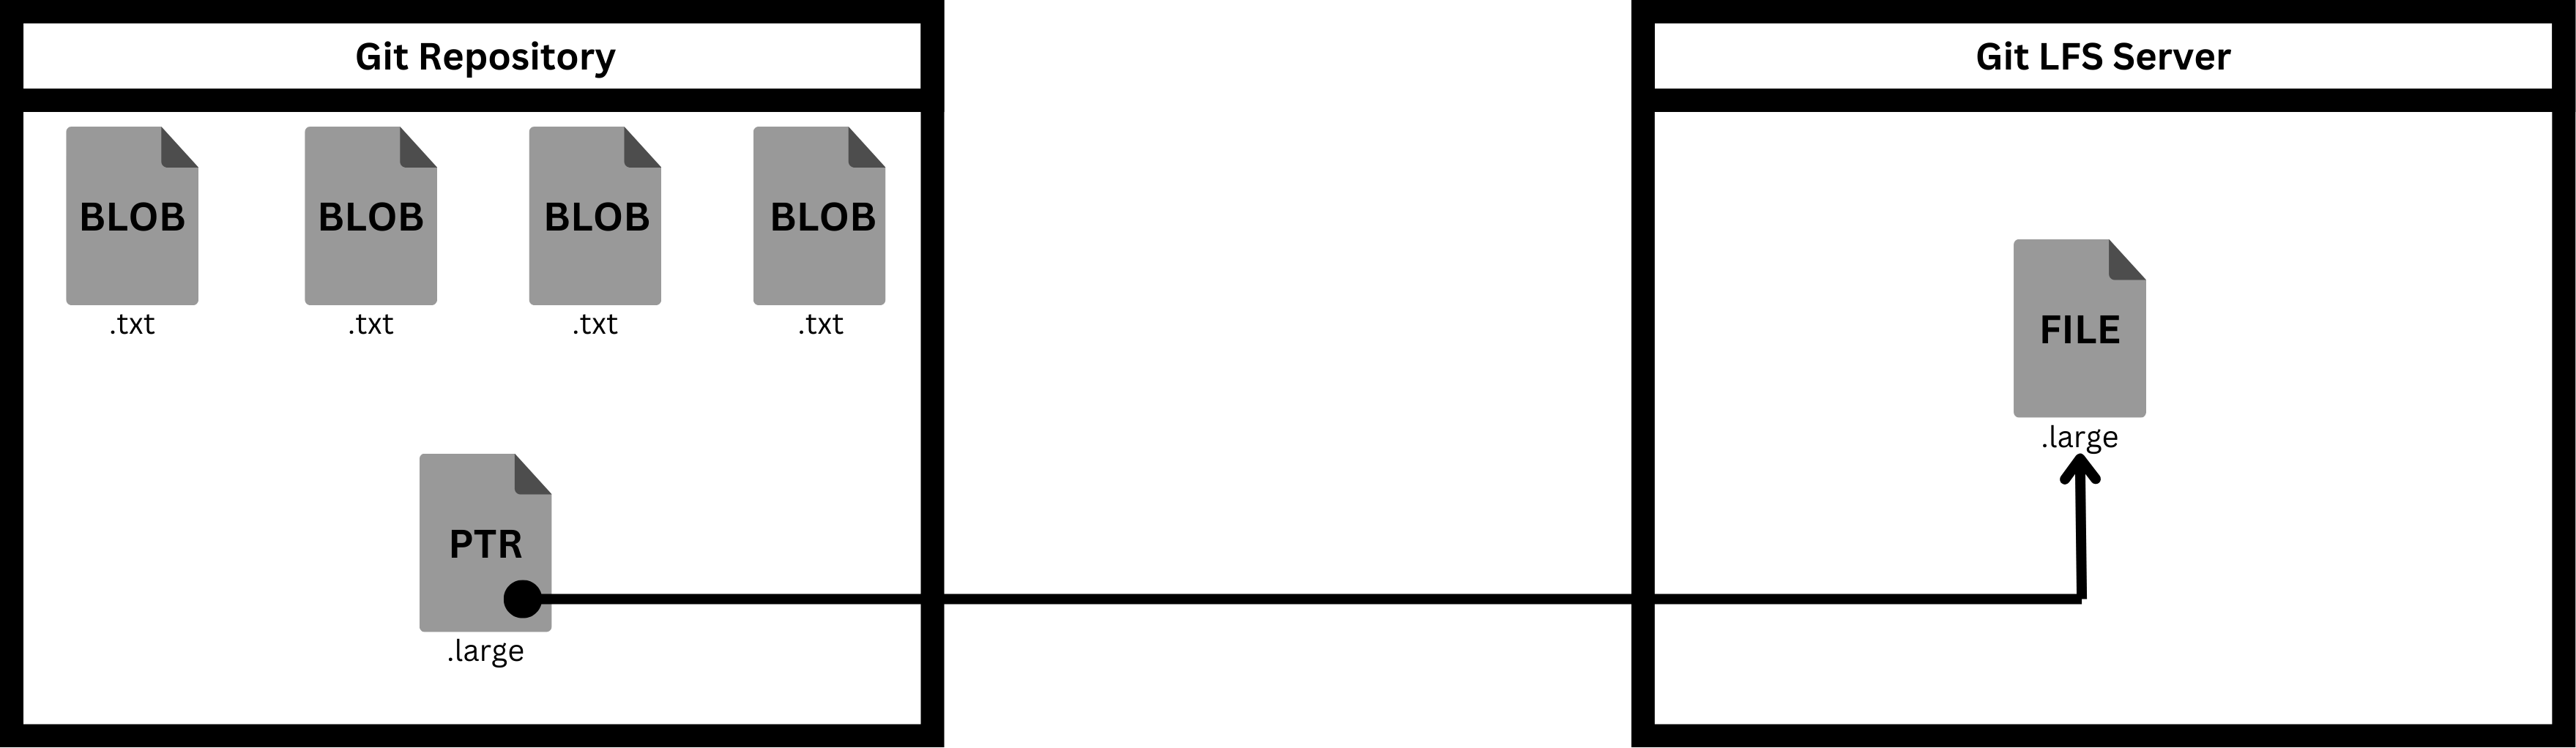
\includegraphics[width=0.8\linewidth]{figs/lfs-pointer.png}
    \caption{Explicative image that shows how LFS establishes a pointer to the remote LFS server.}
    \label{fig:LFSPointer}
\end{figure}

Whenever a branch containing the large file is checked out, its contents are downloaded from the LFS server. In case the contents of the file are modified, the new version of
the file is uploaded to the LFS server, which in turn generates a new version of the pointer file and makes a request to store it at the repository, all of it made in a 
transparent way for developers.

\begin{figure}[H]
    \centering
    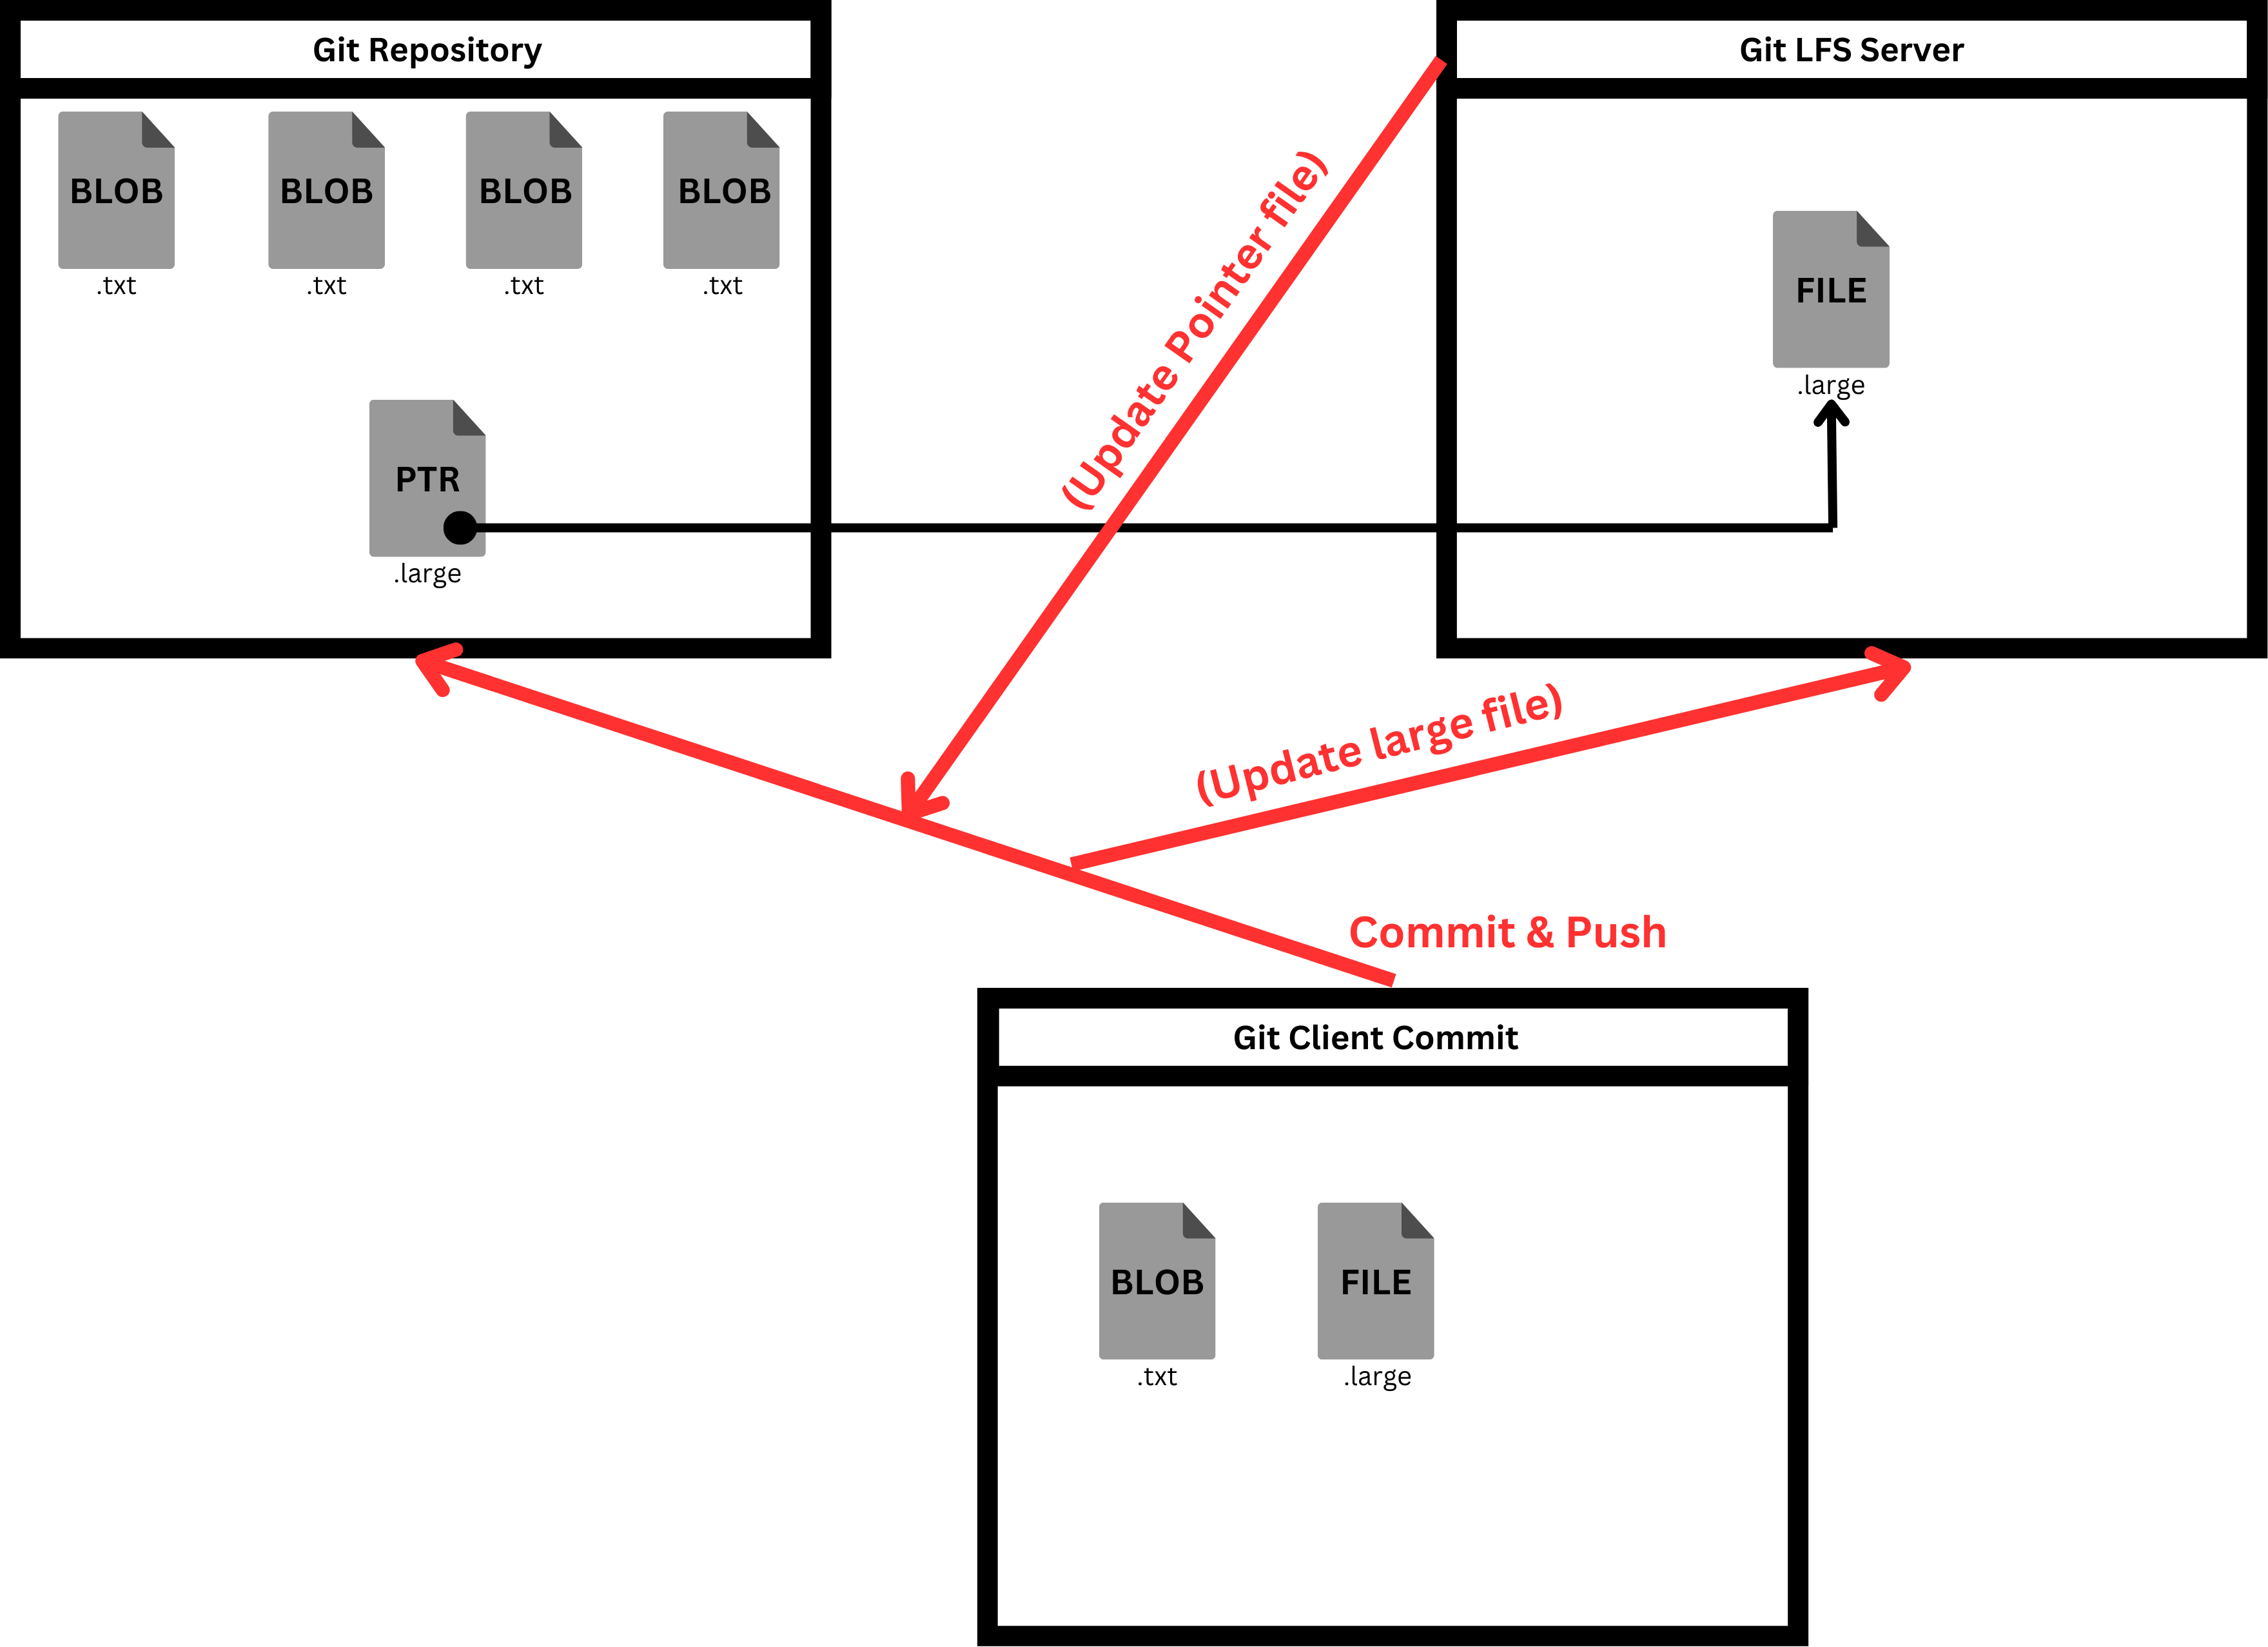
\includegraphics[width=0.8\linewidth]{figs/lfs-commit.png}
    \caption{Diagram of the process LFS performs to carry out the commit operation over a registered large file.}
    \label{fig:LFSCommit}
\end{figure}

With this simple mechanism, it is possible to transparently version and store large files in a Git repository without causing a huge overhead when performing operations at 
the Git repository.

\newpage
\subsubsection{Advantages and disadvantages of Git LFS}

\paragraph{Advantages of Git LFS}

\begin{itemize}

    \item \textbf{High Performance}: The mechanism for storing large files (a few gigabytes large) in Git enables the management of these kind of files as well as not letting
    their size slow down the transactions or using too much memory.

    \item \textbf{Ease of use and familiarity: }The Git LFS command line interface is simple and easy to use for users already familiar with Git, given the similarity between 
    the commands of both interfaces. This considerably flattens the learning curve of the tool.
\end{itemize}

\paragraph{Disadvantages of Git LFS}

\begin{itemize}

    \item \textbf{Not scalable:} If Git LFS were to be used in a distributed environment, it would not scalable due to the fact that it needs to be installed on every end user's
    system, and configured for every repository.

    \item \textbf{Limited in storage:} Git LFS has limited remote storage capacity (2 GB per file), falling thus too short on storage capacity for a project like MADTrack, which
    aims to handle datasets whose weight is counted in hundreds of gigabytes

    \item \textbf{Performance loss for very large files:} According to a Git LFS blog in Assembla \cite{assemblagitlfs}, some performance losses were reported upon storing 
    multiple very large files in a single Git LFS server. This serves as proof that Git LFS has difficulty in managing files heaver than a few gigabytes.

    \item \textbf{Difficult integration:} For integrating Git LFS into a system, it is also required to have Git Credential Manager installed (as a dependency).
    This dependence makes it a less modular solution than other possible alternatives.

\end{itemize}

\subsection{Data Version Control (DVC)}

Data Version Control (DVC) is an open-source, data-science-specialized software tool that provides mechanisms for easy data and experiment management, as well as 
for Machine Learning pipeline automation. It can be used in the form of an \acrfull{IDE} extension, a command line interface, or even as a library of the Python
programming language. It is designed for aiding data science and machine learning teams.

\subsubsection{How does DVC work?}

According to its official documentation \cite{dvcdocs}, the design of DVC is based on three main principles: codification (being able to define any important aspect
of a Machine Learning project by making use of a metafiles, making room for best practices and engineering toolsets), versioning (it uses the Git workflow to enable 
teams to collaborate and share their work), and secure collaboration (enabling selective collaboration and access to all aspects of a project).

DVC has a very similar feel and workflow as Git, thanks to its operation on top of it. The storage space problem is solved by means of special files: DVC metafiles. 
This files have the dvc extension and serve as placeholders to track data files and directories. Additionally, there are other types of files, like the ones with the 
\texttt{dvc.yaml} extension, which have the purpose of modeling entire Machine Learning projects, or \texttt{.dvcignore} files, which are used to ignore certain files or 
directories. The files in DVC are stored in certain local or remote storage systems, but DVC treats them all under the name of DVC remote.

DVC handles repositories as DVC projects, which are initialized by the use of \texttt{dvc init}. Once a project is initialized, DVC offers a wide-ranging variety Of
mechanisms to handle the configuration of the files and directories from a dataset. The \texttt{dvc add} command must be used for tracking an item.

Upon adding an item into DVC's tracking system, both a placeholder named \texttt{<filename>.dvc} will be created, as well as a \texttt{.dvcignore} file (if not
existing yet) within the target's directory. The former will store the changes on the file or directory, whilst the other will prevent the original file or directory from
being tracked by Git.

Furthermore, DVC is also able to retrieve or push data from or to a specific DVC remote using the \texttt{dvc pull/push} command, and to load a previous version of a tracked 
item after a checkout on the Git repository has been made, by making use of \texttt{dvc checkout}.

\subsubsection{Advantages and disadvantages of DVC}

\paragraph{Advantages:\cite{dvcoverview}}

\begin{itemize}
    \item \textbf{Specialisation: } DVC differs from other more general toolsets by its specialisation in the niche opened by emerging ML frameworks. DVC is aims to be used 
    by Machine Learning teams for Artificial Intelligence and Data Science projects. Hence, the options provided by the tool easily adjust to the needs of these specialists.

    \item \textbf{Easy to learn: } DVC working on top of Git repositories and taking inspiration of their workflow makes it very easy to learn and understand. Most of DVC's 
    commands are alike to those of Git.

    \item \textbf{High performance: } DVC has been designed to easily manage files the size of an actual neural networks dataset or a machine learning model. Hence, it makes
    it very efficient for these specific cases.

    \item \textbf{Compatibility: } DVC's remotes can be either local directories or remote storage systems. This may facilitate integration with the existing storage providers
    of the company.

\end{itemize}

\paragraph{Disadvantages:\cite{dvcoverview}}

\begin{itemize}
    \item \textbf{Slightly inflexible: } DVC will not accept an organisationally undefined environment in terms of architecture or design of the Machine Learning workflow. Teams must have a 
    well-defined pipeline and metrics of the model in order to take full advantage of DVC's modeling tool.

    \item \textbf{Workflow imposition: } DVC requires a Git workflow. This makes it very difficult to use the tool in projects where this workflow is not well-suited.

\end{itemize}

\subsection{MLFlow}\label{sec:mlflow}

MLFlow is an open-source project, specifically built with the objective of providing assistance in the Machine and Deep Learning process, managing the full lifecycle of 
projects of this nature and ensuring its traceability and reproducibility\cite{mlflowdocs}.

MLFlow offers mechanisms for Machine Learning model tracking and registry (handles configuration management), evaluation (it is able to track and compare different 
versions of a model) and reciping (provides guiding for structuring a Machine Learning or Deep Learning project).

This tool has gained particular popularity, since it is being used by the great companies, such as Microsoft, META and TOYOTA.

\subsubsection{How does MLFlow work?}

MLflow has a complex workflow consisting of various components, which are thoroughly explained in the following paragraphs \cite{mlflowtracking}.

The MLFLow tracking \acrfull{API} is present in many programming languages (Python, R, Java and REST) and is part of the many components of MLflow, having the aim of 
providing the sufficient logging mechanisms for tracking a \acrshort{ML} or \acrshort{DL} project, including logging of parameters, code versions, metrics and output files.

In figure \ref{fig:MLFlowScenarios}, an overview of the most common MLFlow deployment architectures show the different possibilities MLFlow can be used:

\begin{figure}[H]
    \centering
    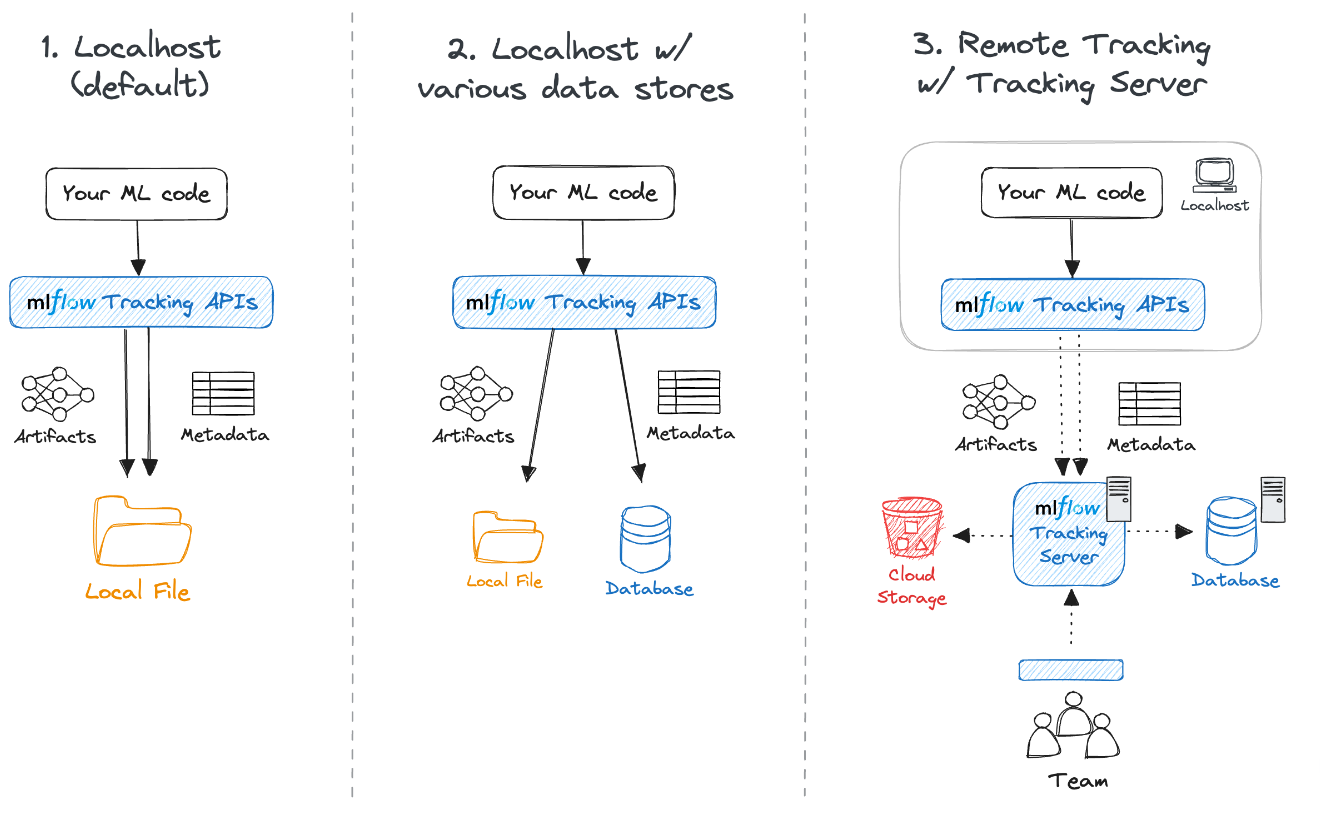
\includegraphics[width=0.8\linewidth]{figs/mlflow-tracking.png}
    \caption{Diagram showing the different use scenarios of MLFlow. Source:\cite{mlflowtracking}}
    \label{fig:MLFlowScenarios}
\end{figure}

In total, three use scenarios can be identified:

\begin{itemize}
    \item \textbf{Localhost scenario: } MLflow stores and logs ML model metadata and artifacts inside a local file system directory.
    
    \item \textbf{Localhost with data stores: } Similar to the previous setup, but it also stores and logs data files in a remote file
    system or database.

    \item \textbf{Use of a remote tracking server:} The ML code is tracked by the API into a remote HTTP tracking server, which stores 
    it in a remote storage and allows storing and retrieving items without directly accessing the storage media.

\end{itemize}

Apart from the API, there are more relevant components, such as the model registry. MLFlow's model registry provides the MLflow toolset 
with mechanisms for model lineage, versioning, aliasing, tagging and annotation. This component of MLflow can be accessed by running a 
proper MLflow server and using a backend storage medium. Whenever a model is desired to be registered, it is needed to be logged first.
Some basic concepts to understand how this registry component works are:

\begin{itemize}
    \item \textbf{Registrable model: }a model created from an experiment or run and logged with one of the model methods. Currently, MLFLow supports SKLearn, Pytorch and
    TensorFlow models.

    \item \textbf{Registered model: }a model registered with using the model registry. It contains a unique name, versions, aliases, tags and metadata.
    
    \item \textbf{Model version: }representation of a stage in the evolution of a model. Any newly registered model is assigned version 1.
    
    \item \textbf{Tag: }quality or set of qualities expressed about a model, expressed as a key-value pair. Allows model categorization.
    
    \item \textbf{Alias: }is a mutable, named reference assigned to a model version.
    
    \item \textbf{Annotation: }Markdown styled comment on a model in any model version. It used for describing and expressing relevant 
    information to the project's collaborators.
\end{itemize}

MLFlow also provides its users with a friendly \acrfull{UI} that is available on the cloud, and accessible by means of an internet browser. Before coming in detail
about the provided functionalities, some concepts may be introduced first:

\begin{itemize}
    \item \textbf{Model run: }process that englobes the training, validation and testing of a model.
    \item \textbf{Experiment: }representation of a set of model runs that share a common purpose, e.g. An experiment for ship segmentation models.
    \item \textbf{Artifact: }a file whose content is relevant to a certain model run.
\end{itemize}

This interface allows the navigation through the different registered experiments using a stack panel, as well as a comparative stack view of the different model runs, 
along with the parameters, metrics and datasets obtained within each run, which can be sorted according to the users' needs. The interface also provides menus for 
visualizing the different models and artifacts within a model run.


\begin{figure}[H]
    \centering
    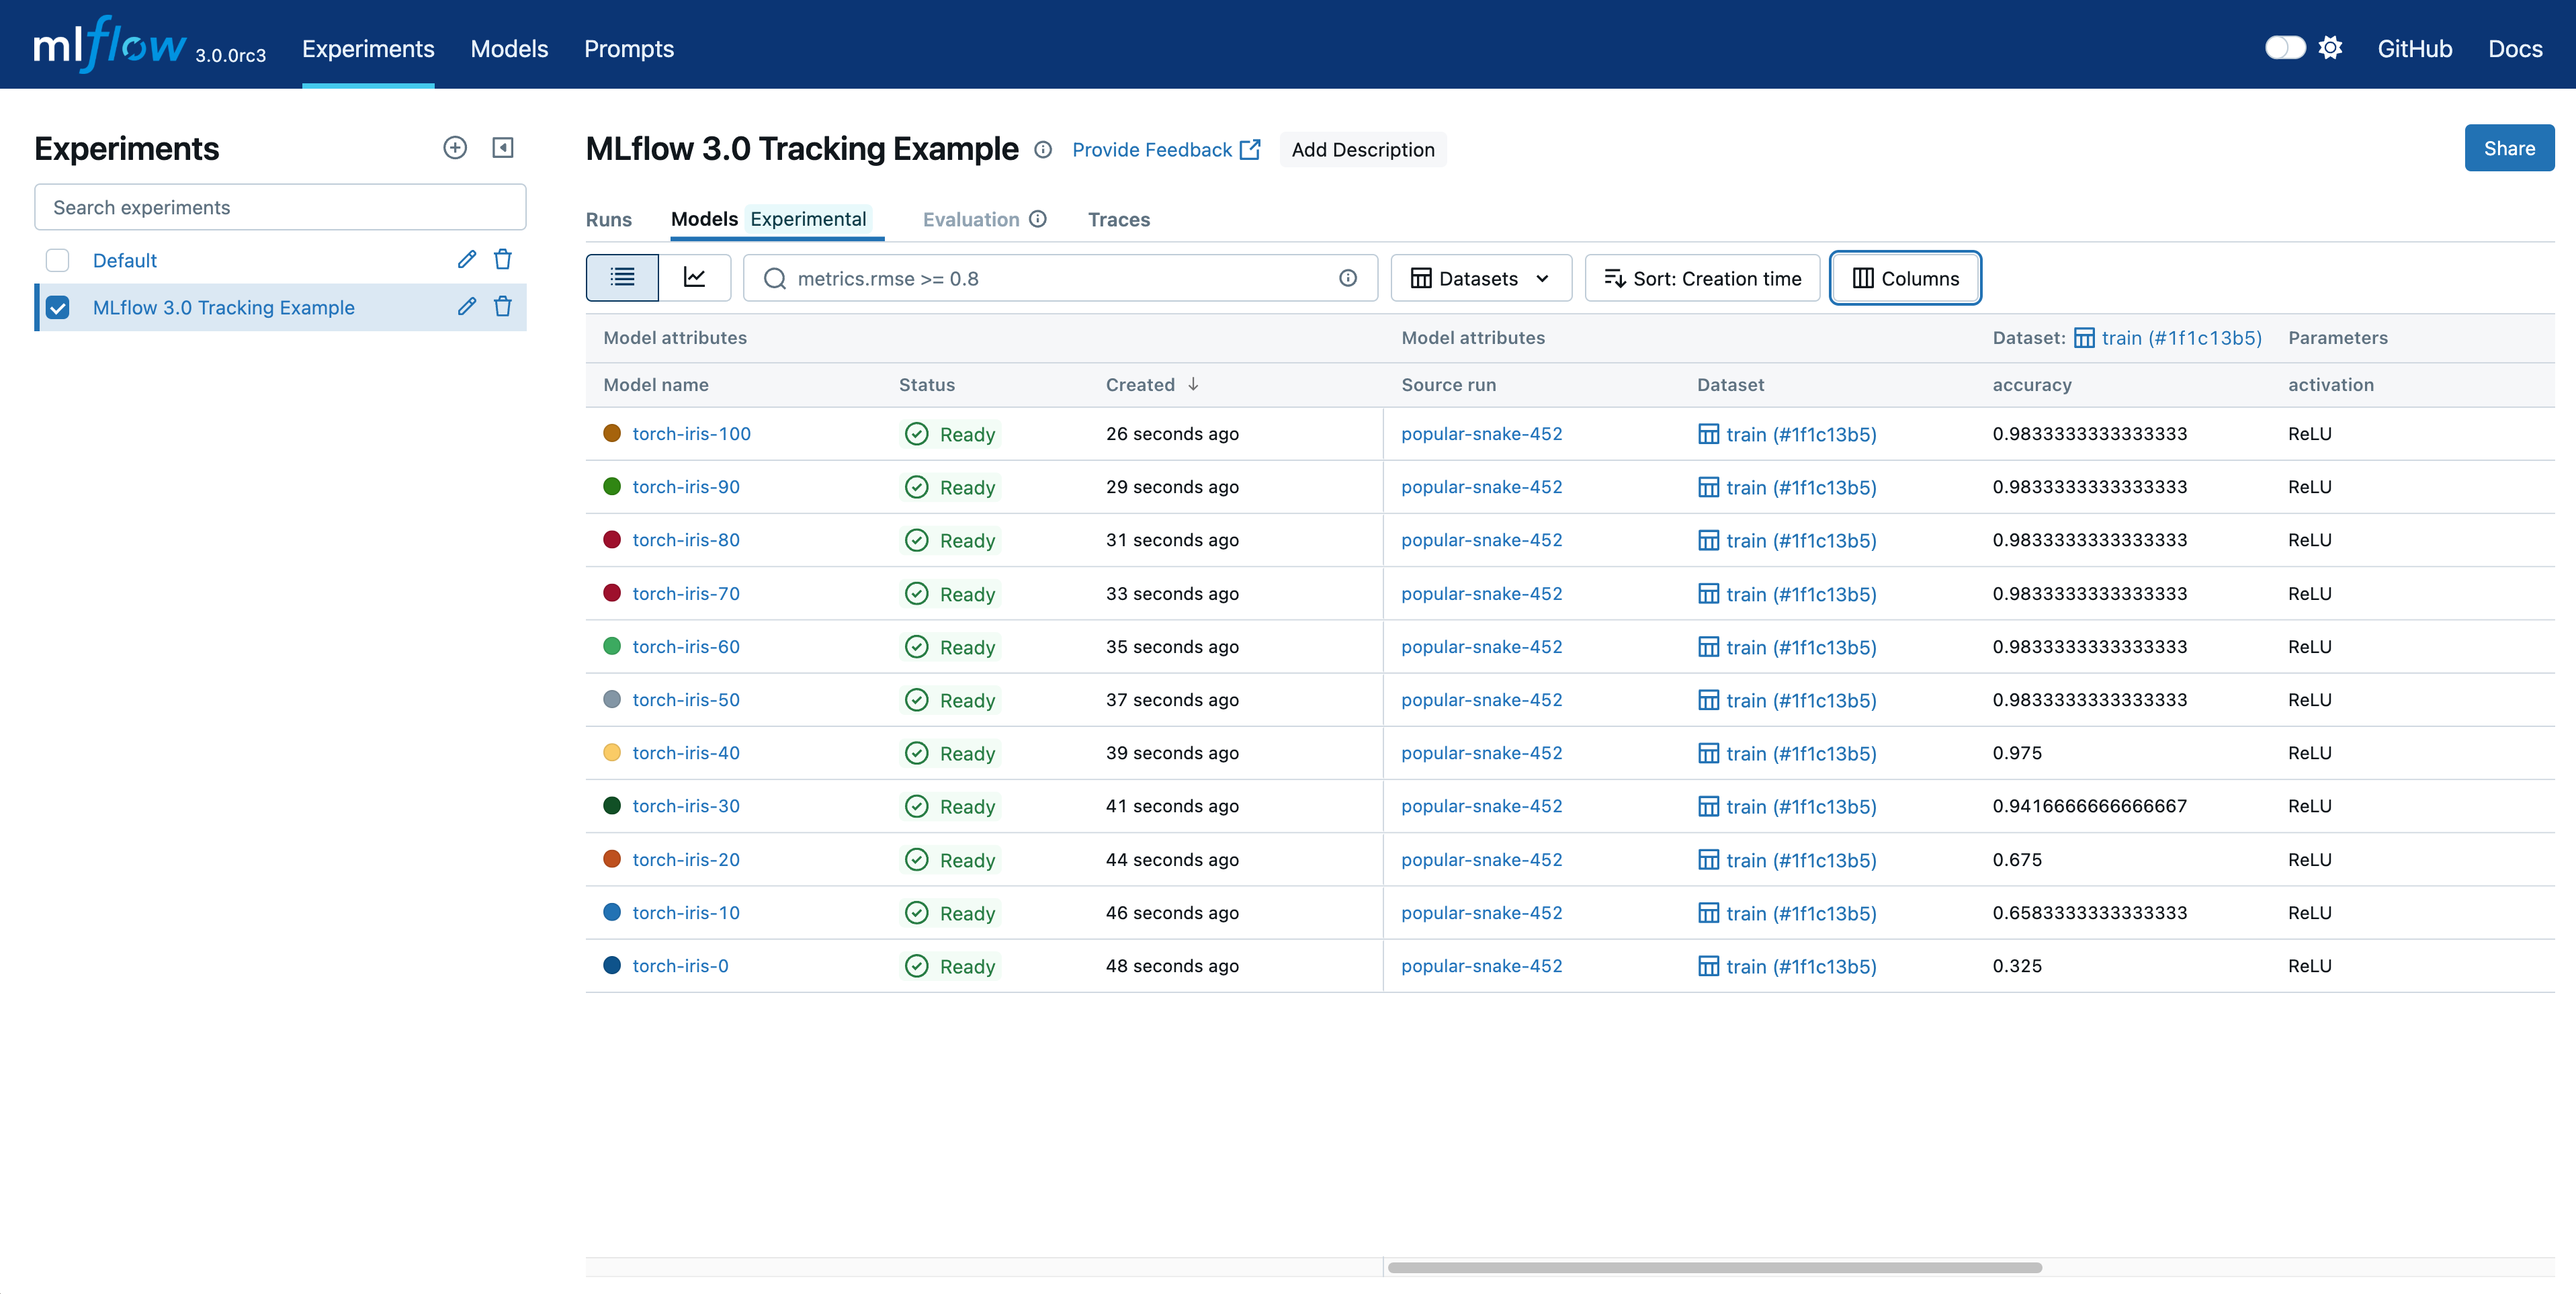
\includegraphics[width=0.8\linewidth]{figs/mlflow-ui.png}
    \caption{MLFLow's \acrshort{UI} showing the list of runs contained within an experiment. Source:\cite{mlflowtracking}}
    \label{fig:MLFlowUI}
\end{figure}

\subsubsection{Advantages and Disadvantages of MLFlow\cite{mlflowproscons} }

\paragraph{Advantages:}

\begin{itemize}
    \item \textbf{Complete: }this tool excels at managing \acrshort{ML} and \acrshort{DL} models, with all the complexity it takes for tracking 
    their evolution, versioning and even comparing them with other models.

    \item \textbf{Easy to learn: }apart from all the complexity hidden for managing the components of the tool, MLflow has an easy installation method
    and an intuitive \acrshort{UI}. The documentation provides users with a wide-ranging set of quick tutorials that will help them get started in the
    minimum amount of time.

    \item \textbf{Flexibility: }in the documentation, it is possible to see many tutorials which import libraries libraries related to the Machine Learning 
    toolset with MLflow libraries, showing its versatility and integrability with many other toolsets related to Artificial Intelligence development. 
    A quite desireable quality for a tool with this role inside a \acrshort{ML} project.
\end{itemize}

\paragraph{Disadvantages:}

\begin{itemize}
    \item \textbf{Insufficiency in dataset management: }MLflow may be a great tool for managing the whole lifecycle of projects and \acrshort{AI} models, 
    but it lacks of mechanisms this good for dataset configuration management. This means that either way, another tool that manages specifically the datasets' lifecycle
    is needed, leading to integration, which leads in turn to higher complexity.

    \item \textbf{Difficult to dominate: }MLflow provides its users with many tutorials to give them a sense of how this tool works in record time. Nevertheless,
    the fact that the tool has a steep learning curve is undeniable. Its varied set of components makes it a complex tool with many possibilities, and it is difficult
    to gather the knowledge to master them all.
\end{itemize}

\subsection{Neptune.ai}

Neptune.ai is a \acrshort{PaaS} that allows users to easily supervise and monitor \acrshort{AI}/\acrshort{ML} foundation model trainings and lifecycle. This set of 
functionalities classify under the definition of an \textbf{experiment tracker} application category. The features offered by Neptune include a combination between
a database and and a dashboard, with logging support for machine learning models for Python, mostly like MLflow does, but adding the incorporation of a decent system
for dataset versioning.

\subsubsection{How does Neptune.ai work?\cite{neptunedocs}}

Neptune.ai's system consists of two main components:

\begin{enumerate}
    \item \textbf{Neptune.ai's Python library: }an \acrshort{API} that can be found inside a Python library, used for logging and querying metadata extracted from model
    building. The tool also offers a \acrfull{CRUD} interface for users and workspaces, as well as various monitoring mechanisms.

    \item \textbf{Neptune.ai's web application: }a web application that enables users to visualize, compare, monitor and collaborate in \acrshort{AI} projects.
\end{enumerate}

The interactions between different clients and servers can be described within figure \ref{fig:NeptuneDiag}. As shown, various clients that have Neptune's library installed make request to an
active Neptune Server, where the web application is also deployed in. The interaction between the users and the web application is regulated by the use of the Python library, creating a workspace
for every existing organization, and a project per Machine Learning task.

\begin{figure}[H]
    \centering
    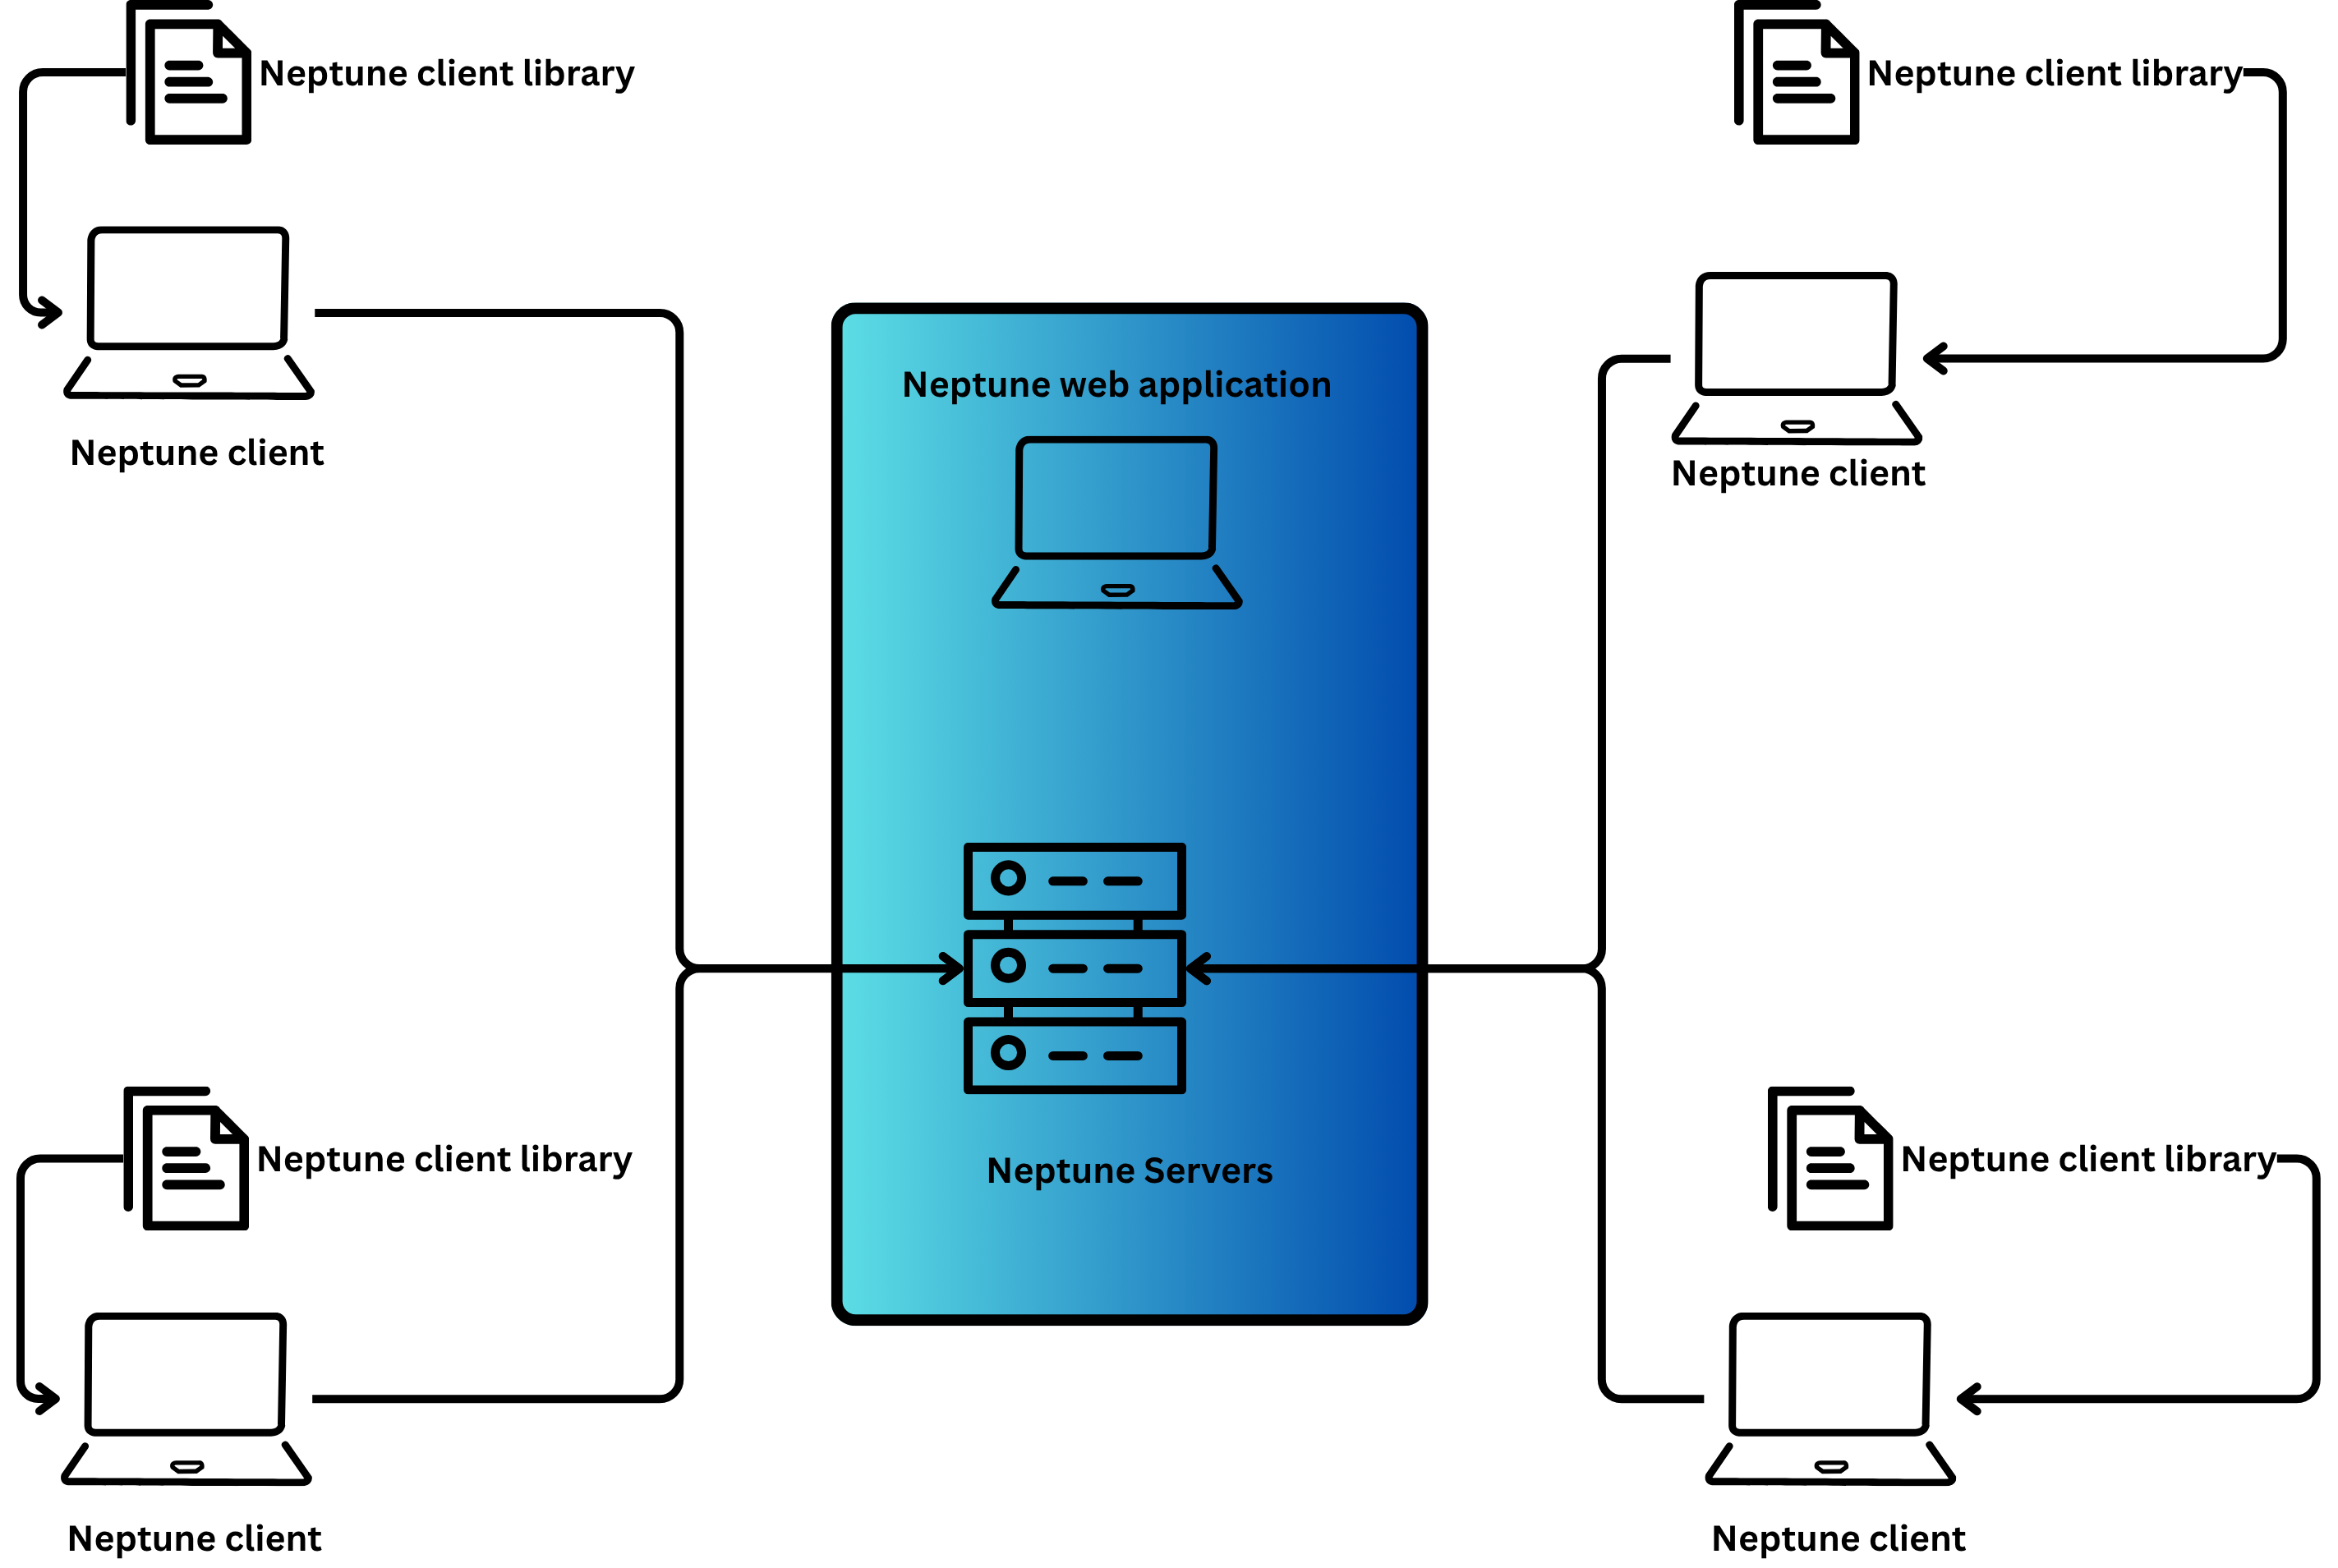
\includegraphics[width=0.8\linewidth]{figs/neptune-clientserver.png}
    \caption{Interaction between Neptune clients and a Neptune server.}
    \label{fig:NeptuneDiag}
\end{figure}

In order to better understand Neptune's environment, some concepts shall be introduced:

\begin{itemize}
    \item \textbf{workspace: }a space for projects and team members with a specific storage amount, created with or without permission for public projects, and with one 
    or more (non-human) service accounts. The storage limits of a workspace can be changed by the workspace administrators, but it may come with a fee charge (The free
    plan of Neptune only provides 200GB storage).

    \item \textbf{Service accounts: }privileged Neptune accounts that do not belong to human entities, and have the purpose of automating tasks that are normally performed
    through a human account. These accounts are workspace-specific and controlled by administrators.

    \item \textbf{Project: }represents the concept of a Machine Learning task. It registers all the tracked runs and shows them to all authorized members, allowing exploration and 
    analysis. Projects have three visibility levels: Workspace (grants access for any of the project's workspace members), Public (available to anyone in the Internet)
    or Private (available only to the chosen members).

    \item \textbf{Run: }a tracked experiment of a project. It contains model-building metadata. They are created every time a model is trained or retrained and
    each time a model performs an inference by means of a executable script.

    \item \textbf{Model: } represents an \acrshort{AI} Model. Is a collection of metadata common to all the model versions of the same model.

    \item \textbf{Model Version: } represents the version of a Machine Learning model. It consists of metadata common to a single version of a model.

\end{itemize}

Neptune also integrates with most of the Machine Learning toolsets available in the market. Making it feasible for integration in the project concerning this Final
Degree Project. It counts with logging callbacks in order to easily integrate it around any model fitting.

Finally, Neptune.ai only takes a little knowledge of environment variables and terminal commands in order to run its \acrshort{UI}, from which all the logging and
metrics can be consulted and the metadata and performance can be easily visualized.

Once the main components of Neptune have been introduced, a generic workflow would have the following steps:

\begin{enumerate}
    \item Add some lines of code before training a model. Just the ones for importing the right libraries and setting the logging callbacks.
    \item Use the Neptune.ai web application to browsed the logged metadata during the training.
    \item Visualize and compare run metadata.
\end{enumerate}

\subsubsection{Advantages and disadvantages of Neptune.ai\cite{neptuneproscons}}

\paragraph{Advantages:}

\begin{itemize}
    \item \textbf{Scoped for project needs: }Neptune.ai manages both models and dataset versioning, so no additional integrations are needed.
    
    \item \textbf{Designed for collaboration: }Neptune.ai is designed to be used in a collaborative environment, so it easily tracks the progress of a project made by 
    any team member.

    \item \textbf{Standardized: }this tool complies with SOC2\cite{SOC2}, a standard for security and compliance.
    
    \item \textbf{Ease of use: }Neptune.ai is a Python API package that can be easily installed and used in any Python project. It also allows the easy visualization the
    metadata of models and their training performance by using the web application.
\end{itemize}

\paragraph{Disadvantages:}

\begin{itemize}
    \item \textbf{Non-scalable: }the tool is not scalable to large datasets as the storage is limited, at least, in the free plan.
    \item \textbf{Limited by language: }The tool only provides a single Python package, which is incompatible with other languages.
\end{itemize}

\subsection{Comet.ml}

Comet.ml is another \acrshort{PaaS} oriented to \acrshort{AI} model evaluation, experiment tracking, and production monitoring, with particular expertise in \acrfull{LLMs}.
It is used by companies like UBER and NETFLIX. It also provides a meeting point for all the \acrshort{ML} development platforms (and even those not aimed
exactly at developing this kind of models) and cloud infrastructure supported by providers like Amazon Web Services, Google Cloud and Azure.

\subsubsection{How does Comet.ml work?\cite{cometmldocs}}

Comet.ml is available as a Python package, a command line extension, and also provides an \acrshort{UI} for visualizing and managing information on experiments.

With the python package,Comet enables logging for three types of information: AI model metadata (key-value pairs, metrics, parameters, information about the system, 
and so on), Assets and data (unversioned files like images, models, confusion matrices), and artifacts (versioned assets, like datasets). Comet.ml will track all relevant
loggable assets until the code execution is over.

The user interface provides an option for customizing dashboard views, as well as for viewing and comparing experiments. It well combines with popular libraries like 
Scikit-Learn, Optuna and the self comet optimizer, helping users to find the optimal set of hyperparameters for their models. Comet also offers a model registry to 
track and version models.

Comet also introduces some concepts such as organization, workspace, project and \acrfull{MPM}. Most of these being equivalent to the definitions provided in earlier
subsections.

\subsubsection{Advantages and Disadvantages of Comet.ml\cite{cometmlproscons}}

\paragraph{Advantages: }

\begin{itemize}
    \item \textbf{Ease of integration: }Comet is easy to integrate with other services and platforms, like Python Flask.
    \item \textbf{User-friendly interface: }Comet has been recommended by some G2 members as a tool with a very intuitive user interface.
    \item \textbf{Suited for collaboration: }Comet is designed for collaborative environments, where multiple members work at a time.
\end{itemize}

\paragraph{Disadvantages: }

\begin{itemize}
    \item \textbf{Costly: }The free plan of Comet.ml is very limited, while the premium plans scale up from 50 dollars a month.
    \item \textbf{Limited Customization: }Comet.ml does not provide as much customization options as other tools, which may be disappointing for the price of the 
    service.
    \item \textbf{Limited by language: }The exclusive availability of the tool in the Python programming language restricts its flexibility.
\end{itemize}

\subsection{Weights and Biases (WandB)}

Weights and Biases, also known as \emph{WandB}, is a \acrshort{PaaS} dedicated to provide data scientists and AI developers with a toolkit that facilitates the production
process of Artificial Intelligence models. It provides support for experiment tracking, hyperparameter sweeping, model registry and workflow automation, among many 
others.

\subsubsection{How does WandB work?}

WandB makes use of a set of lightweight, interoperable tools for managing the configuration of AI models, as well as for storing, displaying and sharing results. This 
makes the platform highly suitable for teams. It is available as either as Python and Javascript libraries, a Command Line Interface (CLI) and an interface that 
functions with an interface specialized in data addition.

Like most platforms, The main workflow consists of adding some code from the libraries prior to carrying out the training process, which connect with the cloud platform,
for later tracking and visualization.

Some of the functionalities offered by WandB are:

\begin{itemize}
    \item \textbf{Experiment tracking: }it allows to track the progress of a project made by any team member.
    \item \textbf{Sweeping: }the platform itself lets developers visualize the impact of the hyperparameters on the performance of the model. The platform is also able to 
    perform open-source algorithms to infer the best possible values for the hyperparameters, visualizing all past and suggested configurations of the hyperparameters
    over a dashboard that the team can visualize.
    \item \textbf{Model Registry: }provides a way to govern over the trained models over their whole lifecycle.
    \item \textbf{Workflow trigger automation: }it offers tools for streamlining the learning pipeline and implementing sophisticated \acrfull{CICD} processes by means of 
    automatic workflow execution.
\end{itemize}

\subsubsection{Advantages and disadvantages of WandB}

\paragraph{Advantages: }

\begin{itemize}
    \item \textbf{Familiarity: }while gathering information to transform it into requirements, process detailed in coming chapters, it was revealed that some of the end users of this project already 
    using this tool.

    \item \textbf{Versatility: }WandB can handle most (if not every) of the steps of the Artificial Intelligence models' lifecycle.

    \item \textbf{User-friendly: }WandB was reported in an article from Netguru\cite{wandbprosandcons} as a tool with a very intuitive user interface.
    
    \item \textbf{Code efficient: }The platform itself requires little amounts of code to be able to carry out the complete WandB workflow.
    
    \item \textbf{Suited for embedded system integration: }WandB can generate reports on power consumption and efficiency over the training and inference processes of 
    an AI model, which can be very useful for embedded AI developers like the intended end users of the project.
\end{itemize}

\paragraph{Disadvantages: }

\begin{itemize}
    \item \textbf{Limited by language: }WandB is only available in Python and Javascript, and not in other languages.
    \item \textbf{Costly: }the free plan of WandB is very limited, while the premium plans scale up from 50\$/month.
\end{itemize}

\section{Adoption of AI and Dataset Configuration Management Technologies}

This page provides the resulting overview from the exploration of other areas or companies that have already adopted a machine learning and dataset versioning platform, 
if possible in a similar context the one intended for this Final Degree Project.

\subsection{Microsoft}
In \emph{section \ref{sec:mlflow}}, it was explained how MLFlow was used by various widely known companies, one of these being Microsoft. This company has indeed 
a section explaining how this tool works in their system and how they use it for integration with another tool: Ray\cite{microsoftmlflow}. Both of them are integrated 
as libraries in Python, and Ray tasks can be logged using the functions offered by MLfLow, thus proving the ease of integration that characterizes MLFlow.

\subsection{WIX}
The cloud website infrastructure and \acrshort{PaaS} provider WIX is a company that, similarly to Microsoft, has chosen to use MLFlow as part of the tools integrated in
the platform (as stated in \emph{section \ref{sec:mlflow}}). They were specially interested in the integration of MLflow and Apache Spark to produce their very own Machine
Learning platform, taking advantage of the model registry component. A deep study of how WIX uses this platform is described in a Medium story\cite{mediumwix}.

\subsection{Edge Impulse}
In 2019, the company Edge Impulse released the platform with the same name into the market. This platform provides a near-to-full range of tools to support Machine 
Learning Operations and Deep Learning pipelines adapted to TinyML, which are embedded systems specialized in or designed for running Machine Learning models. The 
platform provides a set of visual interfaces to make Machine Learning accessible to anyone. Some of its features, like the EON Tuner, also offer support for automated 
operations within the pipeline, thus assuring a more efficient and effective workflow. Up to now, the only limitation or important feature this platform lacks is the 
\acrshort{IoT} device manager and production monitor\cite{edgeimpulse}.

\begin{figure}[H]
    \centering
    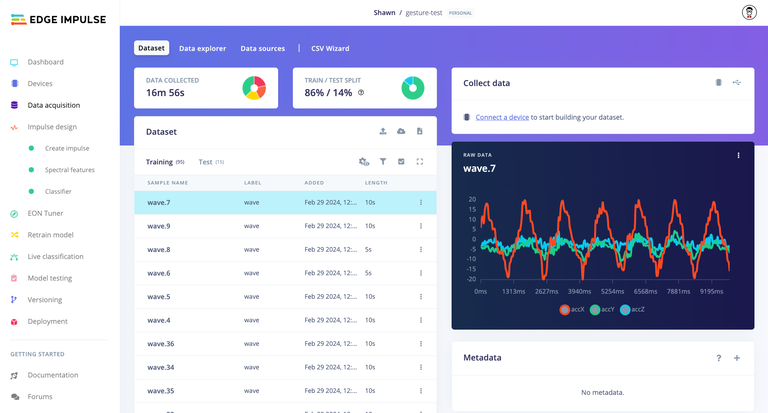
\includegraphics[width=0.8\linewidth]{figs/edgeimpulse-ui.png}
    \caption{A look at Edge Impulse's \acrshort{UI}. Source:\cite{edgeimpulsedocs}.}
    \label{fig:edgeImpulseUI}
\end{figure}


\chapter{Methodology}
\label{cap:Methodology}

This chapter contains details about the followed methodology during the development stages of this project, a time planning for the development stages, the resulting
application of the methodology to this project, and the equipment (software and hardware) used during the development.

\section{Selected Methodology}\label{sec:DSDM}

The selected methodology for the development of this project has been based on the \acrfull{DSDM}, performing some minor adjustments so that the methodology ties in with the project's
needs.

This is an agile framework for software development. It was first published in 1995, with the aim of describing a methodology focused on quality, where the techniques 
for \acrfull{RAD} could be also applied in. The main feature of \acrshort{DSDM} is the use of prototyping techniques to guarantee the frequent delivery of software 
products to the end users\cite{dsdmintro}.

In terms of plannification, most methodologies select to establish a former definition of the desired functionalities to be developed, to then establish a latter time estimation
for the development of each functionality. \acrshort{DSDM}, on the other side, focuses more on establishing a time estimation for the development of the project, in which then the
amount of introduced functionality within the estimated time will be then organized\cite{agileplanning}.

\subsection{Principles of the selected methodology}\label{sec:DSDMPrinciples}

The \acrshort{DSDM} has eight basic principles on which it is sustained. These are:

\begin{enumerate}
    \item Focus on the business needs.
    \item Deliver the artifacts and products on time.
    \item Collaboration among team members.
    \item Build upon a strong basis.
    \item Iterative development.
    \item Continuous and clear communication among stakeholders.
    \item Control during the development of the project.
\end{enumerate}

\subsection{Techniques of the selected methodology}\label{sec:DSDMTechniques}

Throughout the course of the development of the project, \acrshort{DSDM} makes use of a wide-ranging set of techniques, that may be used either alone or in conjunction with
others according to the situation. The most important techniques (which are in fact used in some way in this project) are shown within \emph{figure \ref{fig:DSDMTechniques}},
and detailed within the following subsections.

\begin{figure}[H]
    \centering
    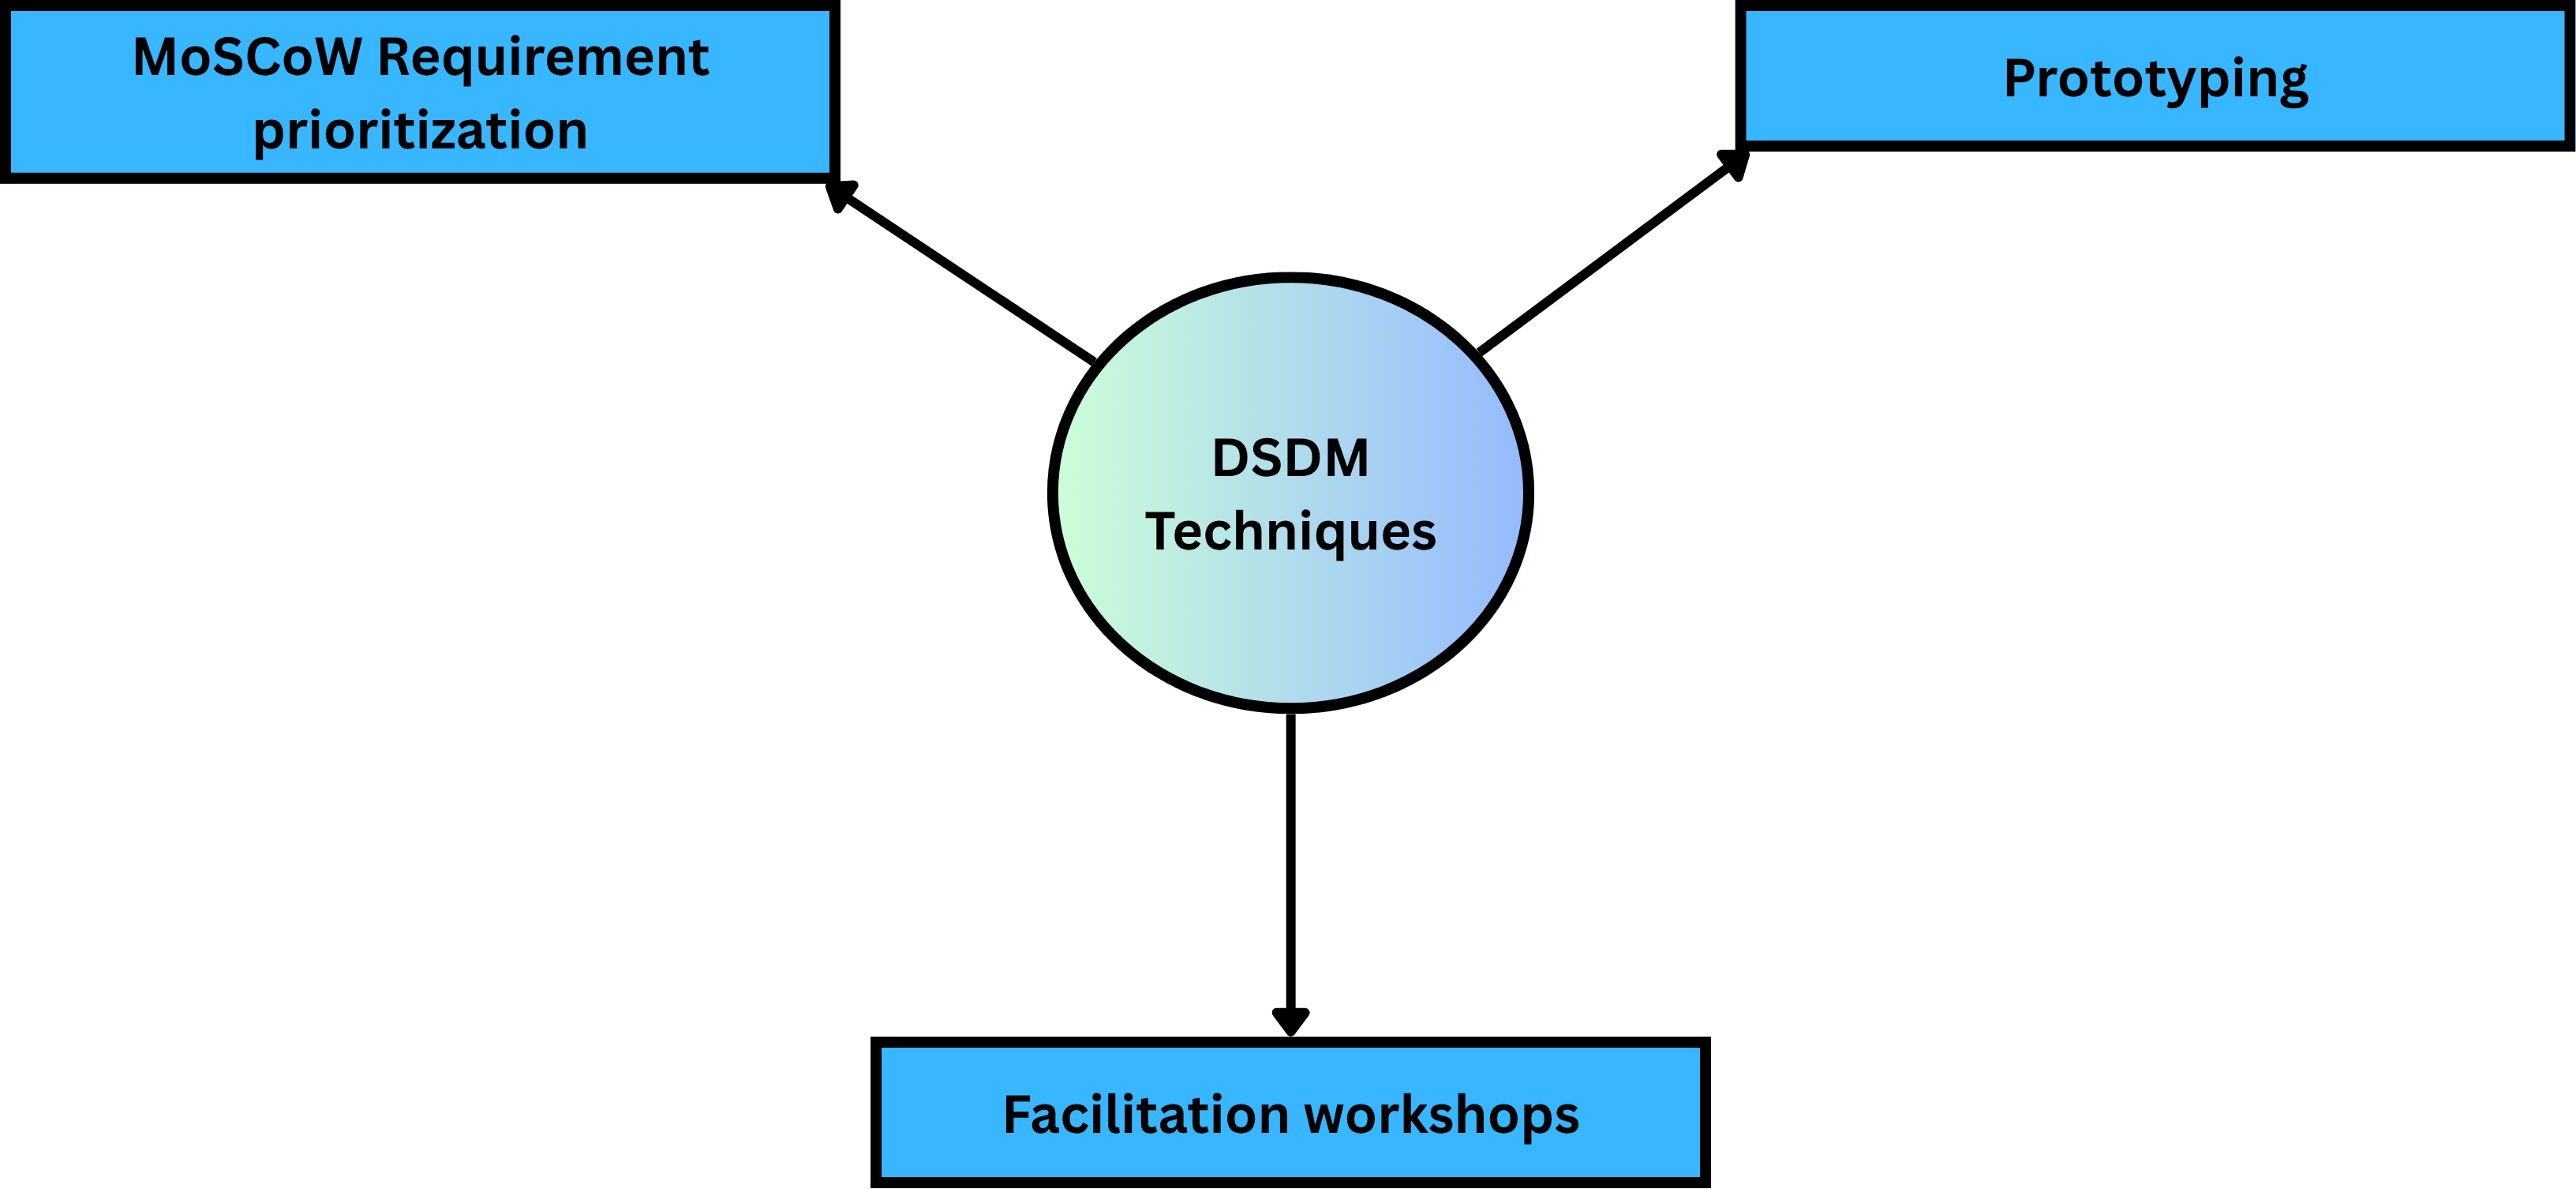
\includegraphics[width=0.8\linewidth]{figs/dsdm-techniques.png}
    \caption{Spider diagram containing techniques widely used in \acrshort{DSDM}.}
    \label{fig:DSDMTechniques}
\end{figure}


\subsubsection{MoSCoW requirement prioritization}\label{sec:MoSCoW}

The MoSCoW prioritization technique was created by software development consultant Dai Clegg in 1994, when teams at Oracle were using \acrshort{RAD} and needed a quick method to
establish requirement priorities. Some years later, in the 2000s, it became a popular technique specially in \acrshort{DSDM}\cite{moscow}.

Prioritization is an essential part of the planning phase of every project. It establishes which of the collected requirements will provide end users with the most value, and
should hence be worked on first. This prioritization is done classifying every single requirement under one of these categories: \emph{Must have}, \emph{Should have}, \emph{Could
have} and \emph{Won't have} (\emph{figure \ref{fig:MoSCoW}}). This classification gives all team members strategic knowledge about the impact of completing (or not) a requirement.

\begin{figure}[H]
    \centering
    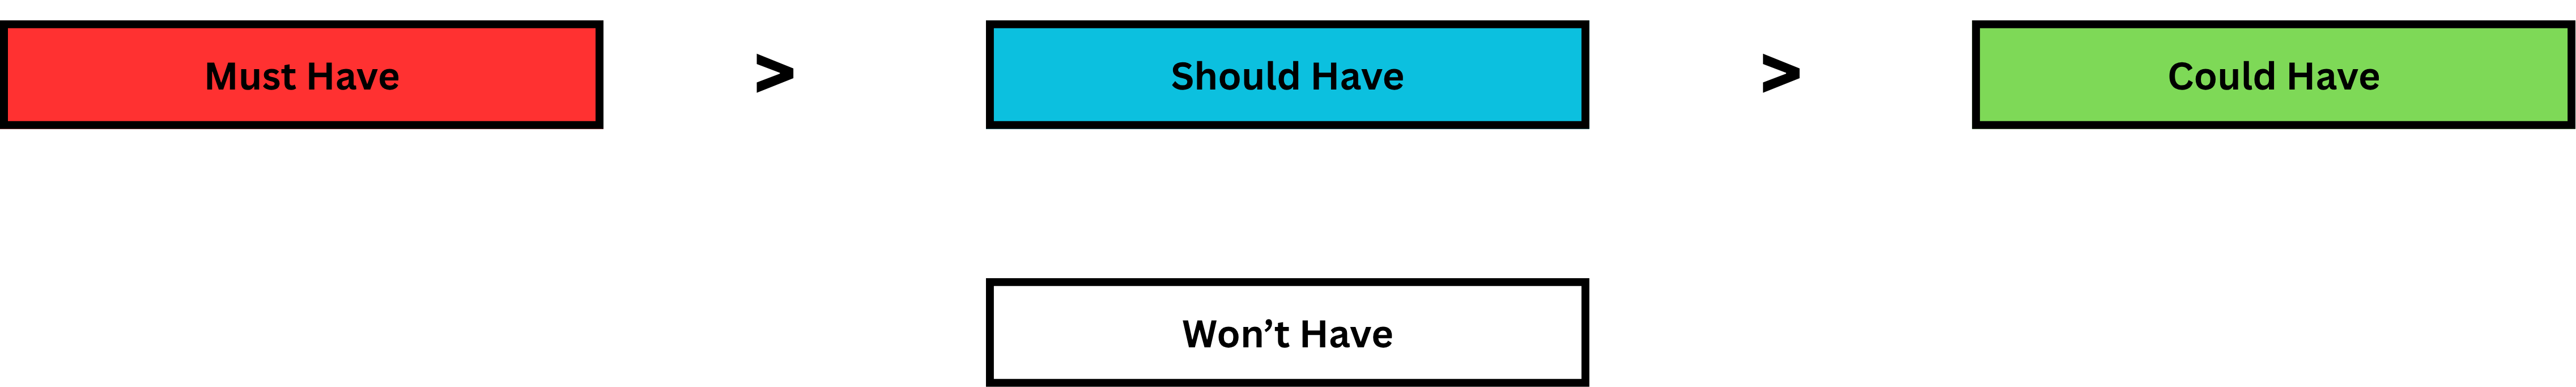
\includegraphics[width=0.8\linewidth]{figs/MosCow.png}
    \caption{MoSCoW prioritization establishes four different priority levels for a requirement.}
    \label{fig:MoSCoW}
\end{figure}

\begin{itemize}
    \item \textbf{Must have: }they are paramount to achieve the project's success. Requirements classified under this category will be the first ones to be completed, since
    they have the greatest importance.

    \item \textbf{Should have: }while they are not essential, they also hold great value for the project, so they should be developed whenever possible.
    
    \item \textbf{Could have: }these requirements are mostly an additive to the baseline of the project, which would increase the satisfaction level of the end users. They will
    only be developed once the baseline is completed, and there are enough time and resources to dedicate to them.

    \item \textbf{Won't have: }this category contains requirements that may hold any importance within the project, but because of limitations on time and resources,
    they will be discarded from the scope of this project's phase. These requirements could be set to be developed in the future phases.
\end{itemize}


\subsubsection{Prototyping}\label{sec:prototyping}

In order to have a shorter delivery interval, \acrshort{DSDM} uses evolutionary prototyping techniques for the development of user requirements.

The main aim of evolutionary prototyping is to carry out a software development production process in an iterative and incremental approach. This means that multiple iterations
of the software development lifecycle will be performed, each of them producing an increment of the system. Although the distinction between products and prototypes in this technique
is fuzzy, the result of the first iterations will be considered prototypes, since they are not near to the full functionality of the final target system\cite{prototyping}.

\subsubsection{Facilitation workshops}\label{sec:facilitationWorkshops}

These workshops are essentially meetings in which the stakeholders of the project meet with a specific objective related to the completion of deliverables. The purpose of the 
workshop is to reach clear solutions to the stated problems.

The development of these workshops is in many ways benneficial for the team:

\begin{itemize}
    \item The workshop is an ideal environment for brainstorming, as well as for discussion and developmen of the produced ideas.
    \item All the stakeholders get knowledge on the decisions made towards the project.
    \item Since all the stakeholders participate in the workshops, they will be able to propose ideas and take part in the decisive process.
    \item The decisions taken during the workshop are quick and precise.
\end{itemize}

\subsection{Project lifecycle in \acrshort{DSDM}}\label{sec:DSDMLifecycle}

The \acrshort{DSDM} methodology divides a project into seven phases to be completed sequentially. These phases are shown within \emph{figure \ref{fig:DSDMLifecycle}}.

\begin{figure}[H]
    \centering
    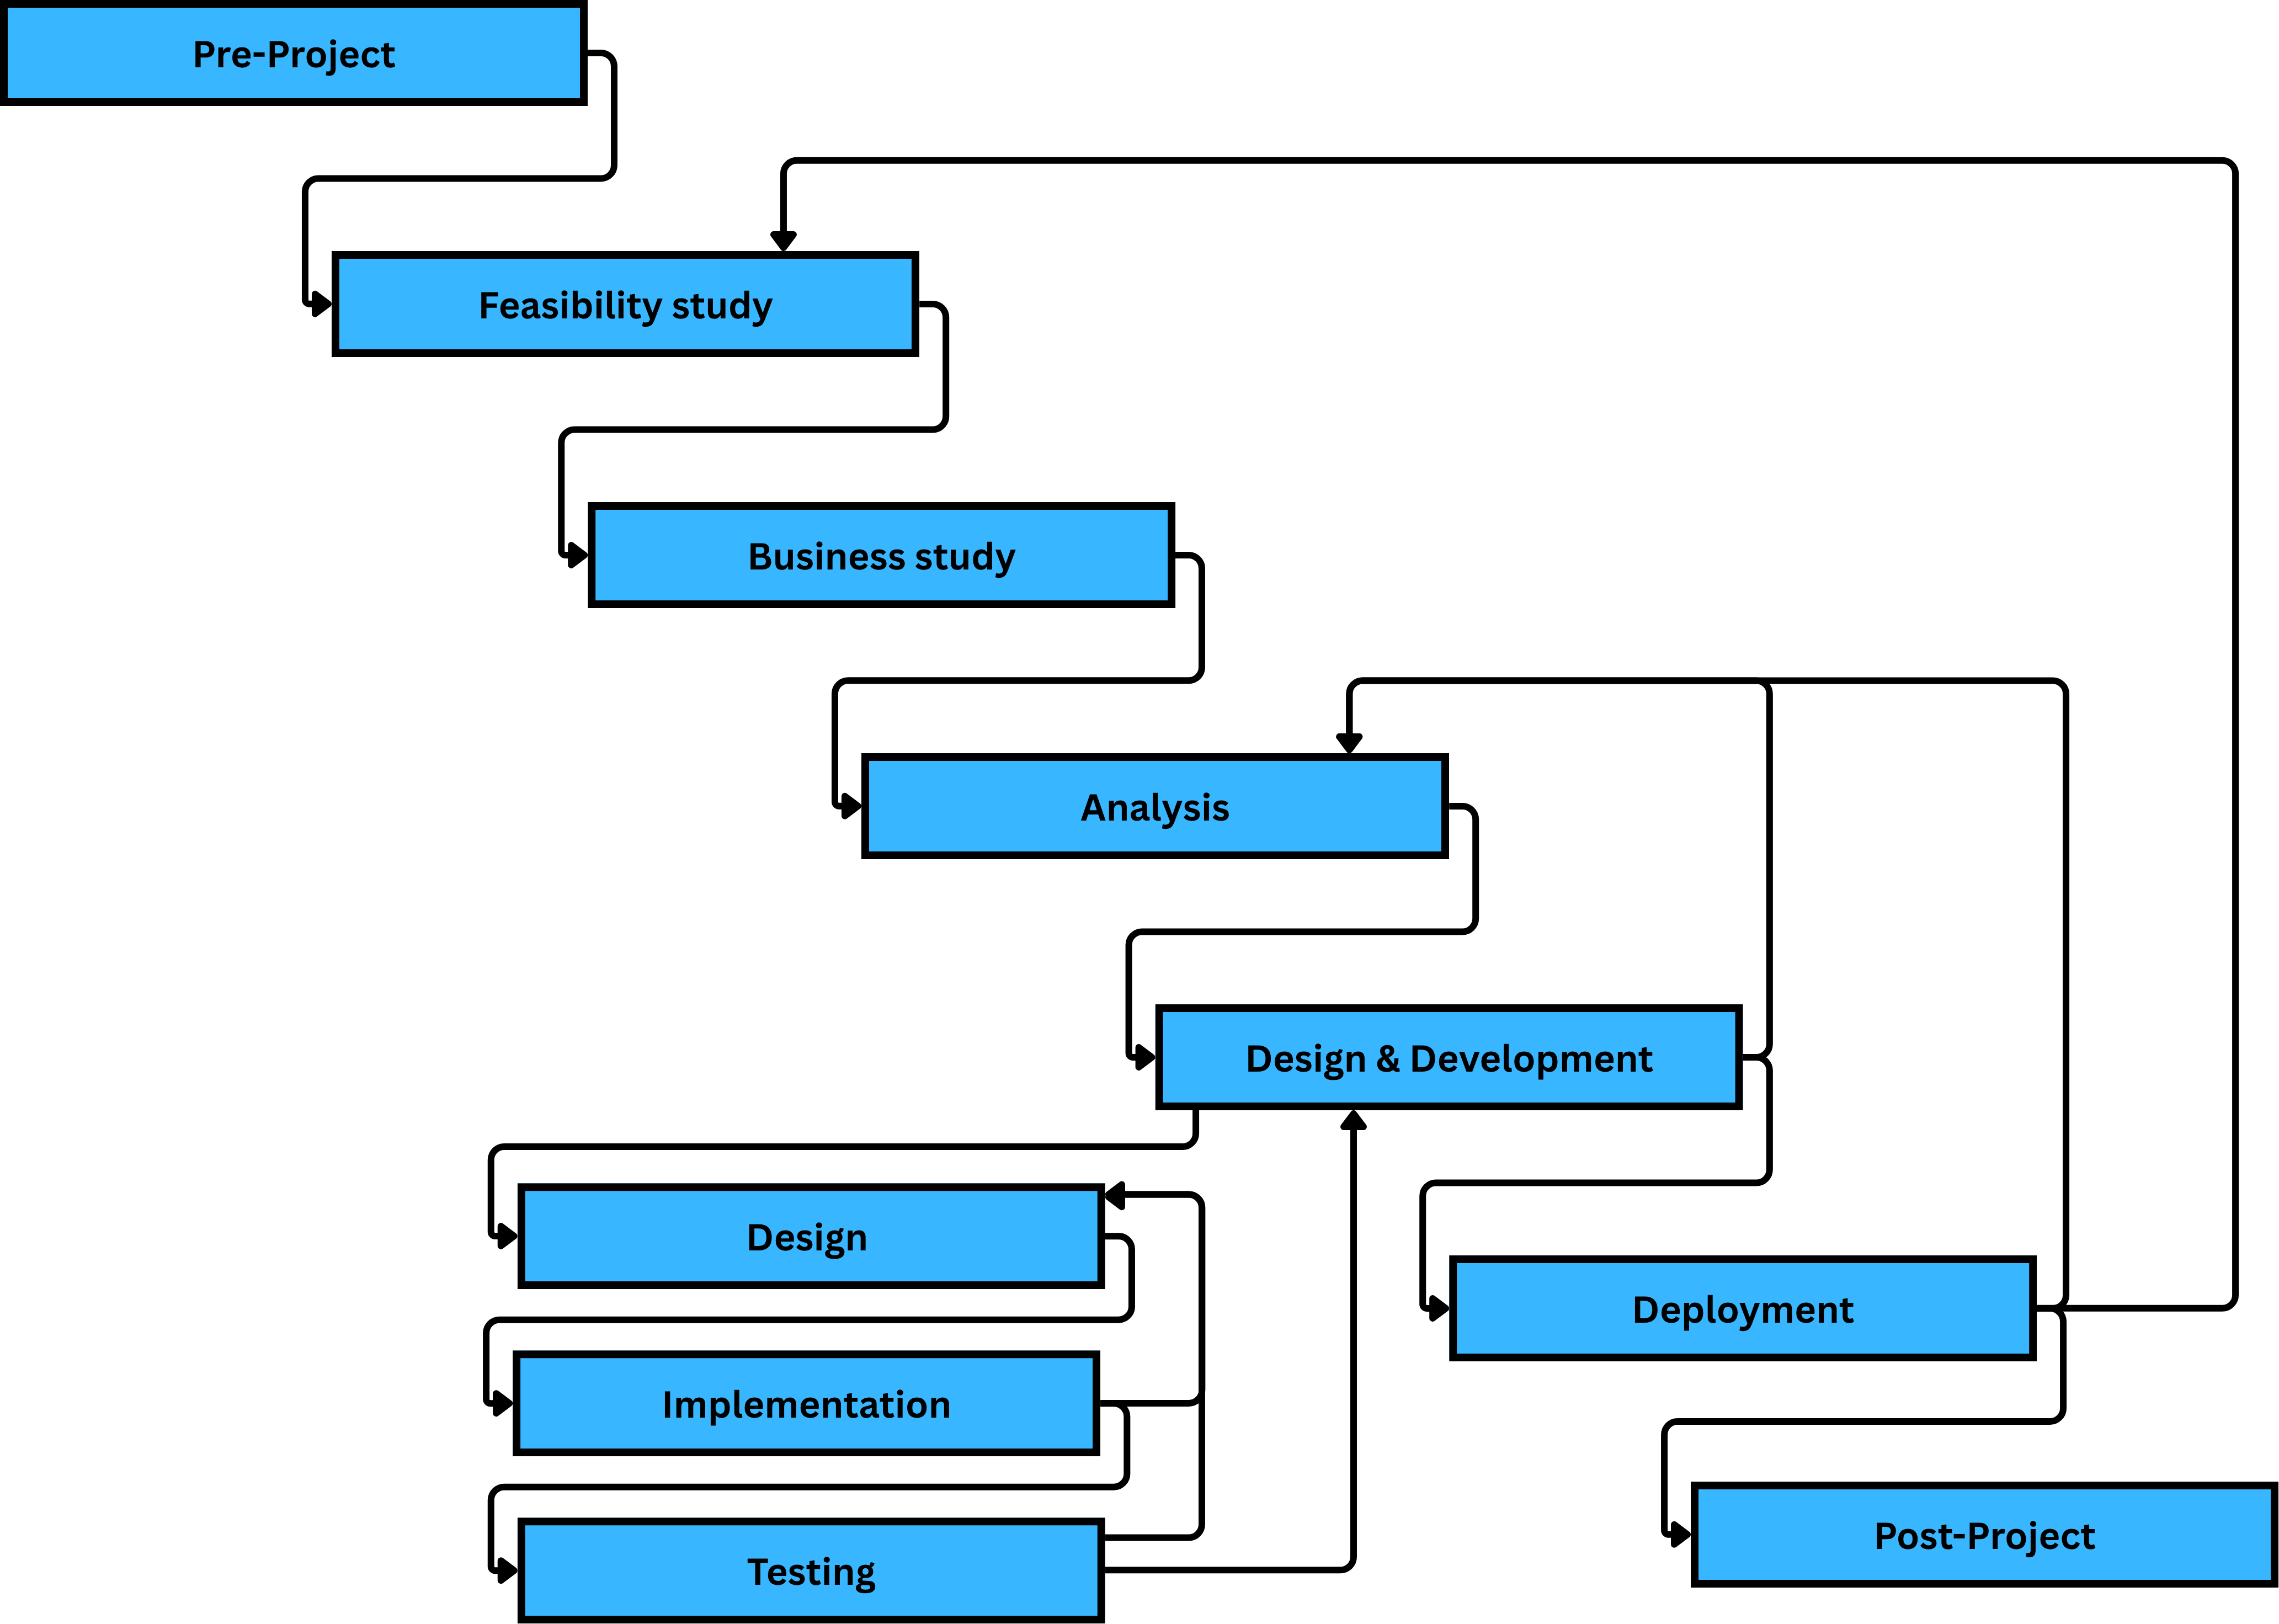
\includegraphics[width=0.8\linewidth]{figs/dsdm-lifecycle.png}
    \caption{The lifecycle of a project, according to \acrshort{DSDM}-based methodologies.}
    \label{fig:DSDMLifecycle}
\end{figure}

\begin{itemize}
    \item \textbf{Pre-project: }this phase has the aim of verifying the establishment of the project over a real need. As well as diagnosing the availability of resources to perform
    a feasibility study.

    \item  \textbf{Feasibility study: }apart from evaluating the adequacy of the use of \acrshort{DSDM} for the development of the project, the techniques to be employed are decided and the
    balance between opportunities and risks upon development is presented. The outputs of this phase include a feasibility report and a provisional project development plan.

    \item \textbf{Business study: }the main aspects of the domain is analyzed, as well as the pontential technologies to be used. The affected business processes are identified,
    along with the components of the target system and the architecture of the system. After this, an initial prototype (which can be far different from the final look of the target
    system) is then created.

    \item \textbf{Analysis: }The first phase of the iterative and incremental development loop. The outputs include a prioritized requirement list, the analysis report
    made on those same requirements, and a risk analysis.

    \item \textbf{Design and development: }the iterative phase where the system is properly built. The low-level component interfaces are designed, to then provide an implementation
    of the system. This phase iterates until obtaining a target system that complies with, at least, the minimal specification formed by the requirements previously agreed.

    \item \textbf{Deployment: }This is the phase englobing the process by which the developed system is integrated within the end user's infrastructure, and consequentially delivered
    to them. On integration, the end user(s) receive a user's manual with all the information needed to correctly make use of the system. Depending on how complex this integration is,
    it is possible to carry out this phase iteratively.

    \item \textbf{Post-project: }After the project ends, an evaluation is made based on whether the specified objectives were satisfactorily fulfilled, and a list of lessons learned is elaborated.
    If some requirements were not fulfilled within the specified time, they could be left for future work on another project.
\end{itemize}

\subsection{Roles in \acrshort{DSDM}}\label{sec:DSDMRoles}

The \acrshort{DSDM} methodology defines fifteen different roles for all the stakeholders of a project. Below, there is an explanation of the most important ones:

\begin{itemize}
    \item \textbf{Developer: }the role assigned to every member of the development team. That is, analysts, designers, programers and testers. These people directly participate
    in the creation of the system, specially within the \emph{Analysis} and \emph{Design and development} phases.
    
    \item \textbf{Technical coordinator: }assigned to those with the responsibility of guaranteeing the quality of the project and defining the architecture of the target
    system.
    
    \item \textbf{Visionary: }assigned to that team member that better understands the business objectives. They have the responsibility of ensuring the rapid completion of
    essential requirements (which according to the MosCow prioritization correspond to the ones labelled as \emph{Must Have}), as well as supervising that the project goes well.
    
    \item \textbf{Executive sponsor: }role assigned to the stakeholders belonging to the end users' organization, and holds the financial power and authority over the project. Stakeholders
    with this role hold great importance in decision-making.
\end{itemize}

\section{Application of the selected Methodology to the project}

This section takes the techniques, phases and roles enumerated and detailed in the previous section to then provide a summary of how and to what extent were they applied
to the project. On first place, the application of the aforementioned roles will be detailed, to then make a summary of the obtained requirements and their acquirement method,
their classification following the MosCoW technique, and how iterations will be classified according to the represented progress type. Finally, the tentative time estimation
per iteration will be presented, along with the actual duration of the iterations.

\subsection{Roles assignation}

According to the role definition made within \emph{section \ref{sec:DSDMRoles}}, the roles within the project have been distributed according to the principles defined in
\acrshort{DSDM}. The resulting assignation is the following:

\begin{itemize}
    \item \textbf{Developer: }the only person to which this role has been assigned is the author of this document, Miguel Ángel Ruiz Arreaza. He is responsible of compiling
    the project's requirements, as well as building the target system. He is considered as multidisciplinary, carrying out the responsibility of an analyst, a designer,
    a programmer and a tester.

    \item \textbf{Technical coordinator: }this role has been assigned to the tutor of this Final Degree Project. He will be in charge of coordinating
    the development and integration and to guarantee the technical quality within this project.

    \item \textbf{Visionary: }the co-tutor of this project has been assigned this role. He will be in charge of coordinating the development
    team with the executive sponsor, so as to assure the alignment and the development of this project with the business interests and objectives.

    \item \textbf{Executive sponsor: }the assignment of this role goes to the \acrshort{CTO} of the end users' company, which has the responsibility of providing the necessary
    resources to develop the project.
\end{itemize}

\subsection{Requirement collection}

The following subsections detail the methodology employed to obtain information about the current state of the configuration management procedures of the end users, as well of
their preferences, needs and working methodologies. Once this methodology is explained, the results obtained from applying it will be described.

\subsubsection{Requirement collection method}

This project has the purpose of creating a system designed to provide value to the target company, which is UBOTICA Technologies. Hence, it is important to consider the needs 
of the employees that work with both \acrshort{ML} and \acrshort{DL} models and datasets, and who have to deal with the difficulty of not keeping track of the state of these. 
For this purpose, a set of interviews were conducted from November 18\textsuperscript{th},2024, to November 25\textsuperscript{th},2024. The selected sample was a group consisting
of six employees working in \acrshort{AI} and \acrshort{CV} tasks close to production environments. Additionally, four of the interviewees also affirmed to carry out research tasks
in environments far from production.

\subsubsection{Requirement collection results}

After conducting the interviews and taking important notes, these are the most important points that should be taken into account for producing a requirement specification:

\begin{itemize}
    \item The end users work at \acrshort{CV}, so the predominating dataset type is the image dataset. The system must do well at managing, moving and changing these.

    \item There is not any official set of important metadata, that are always present within every model or project. The model and project's necessary metadata changes with
    the purpose of the project. This means that the system must be flexible on the amount of metadata to introduce for a certain \acrshort{AI} model or dataset.

    \item Hyperparameters take a particularly important role in model trainings for the end users, since they define important measures, like the length of the image bands and
    the number of colour channels. The system must consider a special form of classifying hyperparameters upon the training of a model.

    \item Upon having two versions of an \acrshort{AI} model, many interviewees selected their datasets along with their labelling distribution, their input hyperparameters, 
    the model architectures and the achieved metrics as the main points of differentiation. This means the system must consider these as the main points of the configuration
    of a model training.

    \item According to most interviewees, new versions of \acrshort{AI} models are stored within a cloud configuration management platform, and registered under a new release. On
    the other side, datasets are stored in a cloud storage platform, separated only by name and with no version tracking, meaning multiple versions of a dataset may coexist within
    the platform, each one occupying its own space. The target system must solve this issue so as to make the storage of datasets more efficient and scalable.

    \item Each time the pipeline of a model training completes successfully, some internal software component of the company automatically generates a PDF report with the main information
    of the training: metrics, performance and the differences with the base model. It would be interesting for the target system to enable the compilation of these reports when model
    trainings are performed. However, this is not true for all the pipelining software tools used within the target company, to the inclusion of this report should be optional.

    \item A particular subject admitted to formerly use the traditional method for storing the configuration of models and datasets, but many inconveniences made them take the decision
    to change to more specialized configuration management systems, such as DVC or WandB. These are technologies mentioned within Chapter 3, and the adoption of a system that integrates these
    will be easier for some workers.

    \item Whilst there are still subjects that denied having much issue when spotting a certain model, all of the interviewed workers assure that downloading datasets is troublesome, either
    due to the download mechanisms of the cloud storage, the location of a dataset within the local file system, the internal company's storage device or the cloud platform, or even by the
    long download time.

    \item Many individuals reported that a checkout system would make the search for a dataset quite more easy and time-efficient.

    \item Some individuals made special emphasis on their need to be able to represent the purpose of the model in some way.

    \item While there are mixed opinions on the inclusion of a parameter tweaking mechanism, the number of subjects declaring this feature out of the scope of the project outnumbers those who
    want it within the system.

    \item Individuals shown particular interest in the inclusion of an \emph{experiment tracking} mechanism within the system, specifically one that can sort the metrics obtained from
    trainings so that users could spot the best-performing model at a glance.
\end{itemize}

After compiling all these important points, a software requirement specification was redacted, being the resulting compilation the one shown in \emph{table \ref{tab:functionalRequirements}}.

\begin{table}[H]
	\centering
	\caption{List of functional requirements of the project (previous to organization and priorization).}
	\label{tab:functionalRequirements}
	\begin{tabular}{ | c | p{12cm} |}
		\hline
		\textbf{Requirement ID} & \textbf{Requirement Description} \\ \hline
		FR1     & The system MUST keep ordered track of dataset configurations. \\ \hline
		FR1.1   & The system MUST detect changes in the size (rows and columns) of datasets. \\ \hline
		FR1.2   & The system MUST keep track of the routes where models and datasets are stored \\ \hline
        FR2     & The system MUST handle the concept of experiments.\\ \hline
        FR2.1   & The system MUST identify an experiment by its identification string, or ID.\\ \hline
        FR2.2   & The system MUST provide a mechanism for creating experiments. \\ \hline
        FR2.3   & The system MUST not Accept an experiment creation request that has no experiment name.\\ \hline
        FR2.4   & The system MUST separate commits from different experiments. \\ \hline
        FR2.5   & The system MUST provide a mechanism for deleting experiments. \\ \hline
        FR2.6   & The system MUST provide a mechanism for switching between experiments.\\ \hline
        FR3     & The system MUST keep ordered track of machine learning model configurations.\\ \hline
        FR3.1   & The system MUST track which dataset was used to train the model.\\ \hline
        FR3.2   & The system MUST track which dataset was used to validate the model.\\ \hline
        FR3.3   & The system MUST track which dataset was used to test the model. \\ \hline
        FR3.4   & The system MUST track the code used for programming the model's training. \\ \hline
        FR3.5   & The system MUST track the configuration of the model's hyperparameters and random parameters used in the training of an AI model. \\ \hline
        FR3.6   & The system MUST track the metrics achieved by an AI model. \\ \hline
        FR3.7   & The system MUST provide users with a mechanism to mark an AI model as currently deployed. \\ \hline
        FR3.8   & The system MUST keep track of the additional parameters used by an AI model if it handles domain-specific data. This will be tested for the domain of Earth Observation (EO). \\ \hline
        FR4     & The system MUST provide a mechanism for evaluating an AI model's metrics' goodness.\\ \hline
        FR4.1   & The system MUST provide a mechanism for choosing policies to evaluate an AI model's metrics' goodness.\\ \hline
        FR4.2   & The system MUST provide a mechanism for identifying the experiment or model with the best values on the chosen metrics.\\ \hline
        FR4.3   & The system SHOULD order the model trainings made on an experiment by the goodness of the values on the chosen metrics.\\ \hline
        FR5     & The system MUST provide a mechanism for visualizing the performance report for a trained AI model (if any).\\ \hline
        FR6     & The system MUST provide a mechanism to visualize the training graph of a model (this is, the graph that describes the progress of the metrics of a model after each epoch).\\ \hline
        FR7     & The system MUST provide users with a mechanism to commit changes to the configuration of an item (both a dataset and an AI model). \\ \hline
	\end{tabular}
\end{table}

Additionally, a list of non-functional requirements was created, based on the needs of the company, these are listed under \emph{table \ref{tab:nonFunctionalRequirements}}.

\begin{table}[H]
	\centering
	\caption{List of non-functional requirements of the project.}
	\label{tab:nonFunctionalRequirements}
	\begin{tabular}{ | c | p{12cm} |}
		\hline
		\textbf{Requirement ID} & \textbf{Requirement Description} \\ \hline
        NFR1    & The system MUST be modular by design. \\ \hline
        NFR1.1  & The system MUST be extensible. \\ \hline
        NFR1.2  & The system MUST be reusable. \\ \hline
        NFR2    & The system MUST be maintainable. \\ \hline
        NFR3    & The system MUST be testable. \\ \hline
        NFR4    & The system SHOULD be power efficient. \\ \hline
        NFR5    & The system MUST be scalable. \\ \hline
        NFR6    & The system MUST maintain transactional integrity. \\ \hline
        NFR7    & The system MUST be fault tolerant. \\ \hline
        NFR8    & The system MUST be flexible. \\ \hline
        NFR9    & The system MUST follow best practices for security. \\ \hline
        NFR10   & The system MUST be usable. \\ \hline
        NFR11   & The system MUST outperform the traditional method for model tracking and downloading (<2h). \\ \hline
	\end{tabular}
\end{table}

\subsection{Requirement organisation and prioritization}\label{sec:requirementOrganisation}

Since this complex project aims to complete an extensive list of requirements, the development team along with the visionary and the technical coordinator decided in a 
facilitated workshop held at January 15\textsuperscript{th},2025, that these requirements shall be reorganized and rearranged by the final specific objective to be
completed. That means the project should be divided into milestones. After performing some analysis, three main milestones were defined for the project to succeed:

\begin{enumerate}
    \item \textbf{Milestone 1 (code \emph{D}):} Development of Dataset Configuration Management features completed.
    \item \textbf{Milestone 2 (code \emph{M}):} Development of Model Configuration Management features completed.
    \item \textbf{Milestone 3 (code \emph{G}):} Development of General Configuration Management features completed.
\end{enumerate}

Given these milestone definitions, the requirement specification was updated so that every functional requirement was classified into one of the milestones. The new 
rearranged requirements would be numbered and identified by the milestone they contribute to, resulting into the specifications shown in \emph{table \ref{tab:requirementsMilestone1}}, \emph{table \ref{tab:requirementsMilestone2}} and \emph{table \ref{tab:requirementsMilestone3}}.

Additionally, these tables incorporate the priorities following the procedures described in \emph{section \ref{sec:MoSCoW}}.

\begin{table}[H]
	\centering
	\caption{List of functional requirements belonging to milestone 1.}
	\label{tab:requirementsMilestone1}
	\begin{tabular}{ | c | p{9cm} | p{3cm} |}
		\hline
		\textbf{Requirement ID} & \textbf{Requirement Description} & \textbf{priority (MoSCoW)} \\ \hline
		DFR1     & The system MUST keep ordered track of dataset configurations.                    & Must have\\ \hline
		DFR1.1   & The system MUST detect changes in the size (rows and columns) of datasets.       & Must have\\ \hline
		DFR1.2   & The system MUST keep track of the routes where models and datasets are stored    & Must have\\ \hline
	\end{tabular}
\end{table}

\begin{longtable}{| c | p{9cm} | p{3cm} |} % La alineación de la tabla ya se define aquí.
    \caption{List of functional requirements belonging to milestone 2.}\\ % Captura para la tabla
    \toprule
    \label{tab:requirementsMilestone2}\\ 
    \textbf{Requirement ID} & \textbf{Requirement Description} & \textbf{priority (MoSCoW)} \\
    \endfirsthead % <-- Cierre del encabezado de la primera página

    % Este es el encabezado que se repite en cada página subsiguiente
    \multicolumn{3}{c}%
    {{\bfseries \tablename\ \thetable{}}} \\ \hline
    \textbf{Requirement ID} & \textbf{Requirement Description} & \textbf{priority (MoSCoW)} \\
    \endhead % <-- Cierre del encabezado para el resto de páginas

    \multicolumn{3}{r}{\textit{Continuing on the next page}} \\
    \endfoot % <-- Pie de tabla para todas las páginas excepto la última

    \endlastfoot % <-- Pie de tabla para la última página

    % Contenido de tu tabla
    \hline
    MFR1     & The system MUST handle the concept of experiments. & Must have \\ \hline
    MFR1.1   & The system MUST identify an experiment by its identification string, or ID. & Must have \\ \hline
    MFR1.2   & The system MUST provide a mechanism for creating experiments. & Must have \\ \hline
    MFR1.3   & The system MUST not accept an experiment creation request that has no experiment name. & Must have \\ \hline
    MFR1.4   & The system MUST separate commits from different experiments. & Must have \\ \hline
    MFR1.5   & The system MUST provide a mechanism for deleting experiments. & Must have \\ \hline
    MFR1.6   & The system MUST provide a mechanism for switching between experiments. & Must have \\ \hline
    MFR2     & The system MUST keep ordered track of machine learning model configurations. & Must have \\ \hline
    MFR2.1   & The system MUST track which dataset was used to train the model. & Must have \\ \hline
    MFR2.2   & The system MUST track which dataset was used to validate the model. & Must have \\ \hline
    MFR2.3   & The system MUST track which dataset was used to test the model. & Must have \\ \hline
    MFR2.4   & The system MUST track the code used for programming the model's training. & Must have \\ \hline
    MFR2.5   & The system MUST track the configuration of the model's hyperparameters and random parameters used in the training of an AI model. & Must have \\ \hline
    MFR2.6   & The system MUST track the metrics achieved by an AI model. & Must have \\ \hline
    MFR2.7   & The system MUST provide users with a mechanism to mark an AI model as currently deployed. & Should have \\ \hline
    MFR2.8   & The system MUST keep track of the additional parameters used by an AI model if it handles domain-specific data. This will be tested for the domain of Earth Observation. & Must have \\ \hline
    MFR3     & The system MUST provide a mechanism for evaluating an AI model's metrics' goodness. & Should have \\ \hline
    MFR3.1   & The system MUST provide a mechanism for choosing policies to evaluate an AI model's metrics' goodness. & Should have \\ \hline
    MFR3.2   & The system MUST provide a mechanism for identifying the experiment or model with the best values on the chosen metrics. & Should have \\ \hline
    MFR3.3   & The system SHOULD order the model trainings made on an experiment by the goodness of the values on the chosen metrics. & Should have \\ \hline
    MFR4     & The system MUST provide a mechanism for visualizing the performance report for a trained AI model (if any). & Should have \\ \hline
    MFR5     & The system MUST provide a mechanism to visualize the training graph of a model (this is, the graph that describes the progress of the metrics of a model after each epoch). & Could have \\ \hline
\end{longtable}


\begin{table}[H]
	\centering
	\caption{List of functional requirements belonging to milestone 3 (expanded due to space availability).}
	\label{tab:requirementsMilestone3}
	\begin{tabular}{ | c | p{9cm} | p{3cm} |}
		\hline
		\textbf{Requirement ID} & \textbf{Requirement Description} & \textbf{priority (MoSCoW)} \\ \hline
        GFR1     & The system MUST provide users with a mechanism to commit changes to the configuration of an item (both a dataset and an AI model).   & Must have \\ \hline
        GFR1.1   & The system MUST Identify commits by their Identification string, or ID.   & Must have \\ \hline
        GFR1.2   & The system MUST provide a mechanism for creating commits.   & Must have \\ \hline
        GFR1.3   & The system MUST not Accept the creation of a commit that does not have a commit title.    & Must have\\ \hline
        GFR1.4   & The system MUST allow users to leave a commit message when building up a commit.    & Must have\\ \hline
        GFR1.5   & The system MUST provide users with a mechanism to push a commit to a certain remote repository location.    & Must have\\ \hline
        GFR1.6   & The system MUST provide users with a mechanism to go back to a previous commit.    & Must have\\ \hline
        GFR1.7   & The system MUST be able to handle two instances of a same dataset or model, in different versions, within the same repository.    & Must have\\ \hline
	\end{tabular}
\end{table}

\subsection{Iteration planning}

According to \emph{section \ref{sec:DSDMTechniques}}, prototyping is one of the main techniques within \acrshort{DSDM}-based methodologies. Hence, the iterations of the development
of the project have been organised according to prototype production. In other words, the output of an iteration of the \emph{Design and development} phase of the project is a project
prototype.

Each prototype will be assigned a subset of requirements of a specific milestone, following the milestone definition made at \emph{section \ref{sec:requirementOrganisation}}. The prototype
(and therefore, the iteration of the project) is considered as completed when all the requirements of the prototype are developed. The development of a prototype may require performing minor
changes on the development of previous prototypes. This fact motivates the definition of a versioning protocol for these prototypes, which will be defined in the following subsection. Right
afterwards, the prototypes will be defined and then arranged into the roadmap of the project.

\subsubsection{Prototype version control protocol}

Given the three milestones defined at \emph{section \ref{sec:requirementOrganisation}}, the name of a prototype will consist of the code of the milestone it corresponds to, 
and the iteration number it corresponds to within that same milestone (e.g., the first prototype for Milestone 3 would be called \emph{G1}).

For any addition to an already-developed prototype related with the requirements contained within it (e.g., a hotfix), semantic versioning will be used.
For instance, if a hotfix is needed to prototype \emph{G1}, the new version of the prototype will be called \emph{G1.0.1}. For minor versions, the second number will be increased. Of 
course, a higher major number for a prototype will indicate that it includes the past prototypes for its milestone\cite{semanticversioning}. If no prototypes have been developed
for a particular milestone at a given moment, the iteration number for that milestone will be considered 0.

The name for a version of the system will be the mixture of all the prototypes present up to the point the version is released. As an example, a version of the system that 
only contains the first prototypes of milestones 1 and 2 would be called \emph{D1M1G0}.

\subsubsection{List of prototypes of the project}

\paragraph{Prototypes for milestone 1}

\begin{itemize}
    \item \textbf{Prototype D1: }Provides the necessary mechanisms for the system to be able to integrate and transparently locate a dataset in the system (establishing a versioning protocol).

    \item \textbf{Prototype D2: }Apart from locating a dataset, the system is able to detect simple changes in the datasets, particularly in the number and content of the features and instances
    contained within them. Additionally, the system will be able to bring a dataset from a specific location to the user.
\end{itemize}

\paragraph{Prototypes for milestone 2}

\begin{itemize}
    \item \textbf{Prototype M1: }this inital prototype is focused on the integration of the concept of \emph{experiments} in the system, being able to create and track multiple 
    experiments, apart from sepparating the progress made among the different experiments.
    \item \textbf{Prototype M2: }once the system is able to differenciate the different experiments, the system must be able to track the different characteristics of a model
    upon training. This involves tracking the used datasets, the hyperparameters used, the metrics achieved, and experiment data related to the domain of application (in the 
    current case, the domain of Earth Observation).
    \item \textbf{Prototype M3: }the system is able to used the historically collected metrics from an experiment in order to extract key information like, for example, which
    of the historically performed experiment runs provided the best performance. Additionally, it provides mechanisms for visualizing both the performance report and the 
    training graph produced by the training of an \acrshort{AI} model.
\end{itemize}


\paragraph{Prototypes for milestone 3}

\begin{itemize}
    \item \textbf{Prototype G1: }The system provides a mechanism for users to commit changes to an item (a dataset or an AI model) in order to store them as historical versions in the system.
\end{itemize}

\subsubsection{Roadmap of the project}

On \emph{figure \ref{fig:roadmap}}, the dependencies among iterations (and hence, the dependencies among the prototypes) are shown. The main dependencies encountered are:

\begin{enumerate}
    \item Prototypes \emph{D2} and \emph{M2} depend both on \emph{G1}, since both of these prototypes generate items that may be of great value to commit. Hence, it would be valuable 
    to already have mechanisms that allow to store the items within a configuration management system. This makes \emph{G1} the prototype on which more iterations depend and, therefore,
    motivates it to be the first one to be completed.

    \item Prototype \emph{M2} depends on prototype \emph{D1}, since the former needs to identify the datasets used upon the training process of a model, and will use whatever versioning
    system is defined at the latter to reference these datasets.
\end{enumerate}

Considering the purpose of the prototypes and their dependencies, the designed roadmap is shown at \emph{table \ref{tab:roadmap}}.

\begin{table}[H]
	\centering
	\caption{Roadmap for the project. For details about the stages and dependencies, see \emph{figure \ref{fig:roadmap}}.}
	\label{tab:roadmap}
	\begin{tabular}{ | c | p{9cm} |}
		\hline
		\textbf{Iteration} & \textbf{Prototypes and Phases involved} \\ \hline
        Iteration 1  & \begin{itemize} \item Milestone 3 Analysis \item Prototype \emph{G1} \end{itemize} \\ \hline
        Iteration 2  & \begin{itemize} \item Milestone 1 Analysis \item Prototype \emph{D1} \end{itemize} \\ \hline
        Iteration 3  & \begin{itemize} \item Prototype \emph{D2} \end{itemize} \\ \hline
        Iteration 4  & \begin{itemize} \item Milestone 2 Analysis \item Prototype \emph{M1} \end{itemize} \\ \hline
        Iteration 5  & \begin{itemize} \item Prototype \emph{M2} \end{itemize} \\ \hline
        Iteration 6  & \begin{itemize} \item Prototype \emph{M3} \end{itemize} \\ \hline
	\end{tabular}
\end{table}


\subsection{Time estimations for the project}

With the clear picture of what prototypes provide more value and have more dependencies, an estimation was made of the 
investment of the time that will be required to carry out each iteration of the project.


\subsubsection{Early time estimation}

A first estimation was made before the beginning of the \emph{Analysis} phase of the project, and can be seen in \emph{table \ref{tab:firstTimeEstimation}}. 
The protototypes are ordered sequentially according to the proposed development order, prioritizing those iterations whose output
prototype constitutes a dependency to others. The higher the number of development order, the further in the timeline the 
iteration shall be scheduled.

\begin{table}[H]
	\centering
	\caption{Time estimations for all the project iterations.}
	\label{tab:firstTimeEstimation}
	\begin{tabular}{ | c | c |}
		\hline
		\textbf{Iteration} & \textbf{Time estimation (Days)} \\ \hline
        Iteration 1     & 15 \\ \hline
        Iteration 2     & 15 \\ \hline
        Iteration 3     & 10 \\ \hline
        Iteration 4     & 15 \\ \hline
        Iteration 5     & 10 \\ \hline
        Iteration 6     & 10 \\ \hline
        \textbf{Total}  & 75 \\ \hline
	\end{tabular}
\end{table}


\subsubsection{Actual time duration}

During the course of the project, the time spent in each iteration differed from the initial time estimation. The actual 
time durations are shown in \emph{table \ref{tab:actualTimeDurations}}.

\begin{table}[H]
    \centering
    \caption{Actual time durations for all the project iterations.}
    \label{tab:actualTimeDurations}
    \begin{tabular}{ | c | c |}
        \hline
        \textbf{Iteration} & \textbf{Time duration (Days)} \\ \hline
        Iteration 1     & 18 \\ \hline
        Iteration 2     & 21 \\ \hline
        Iteration 3     & 9 \\ \hline
        Iteration 4     & 20 \\ \hline
        Iteration 5     & 14 \\ \hline
        Iteration 6     & 9  \\ \hline
        \textbf{Total}  & 91  \\ \hline
    \end{tabular}
\end{table}

The main reason for this 16-day difference is mainly because of prototypes \emph{D1} and \emph{M1}, which required more time to be completed in order for the development
team to be familiarized themselves with the used technological tools used, and finding the ways for them to be integrated within the project. The fact that an initial analysis was also 
included within iterations 2 and 4 is another reason for this difference.

\section{Employed equipment and resources}

A key aspect of the description of the project is not only the techniques used to carry out the development, but also the resources (in this case, hardware and software)
utilized in the process. Coming on this section and its subsections, the details about the different equipment and resources used within the development of MADTrack.

\subsection{Hardware resources}

Hardware resources constitute the set of physical devices and peripherals used to carry out the development of the project.

\subsubsection{Computer}

During the development of the project, the target company provided the development team with a laptop computer. This computer is the main means through which the main programming
were performed, through which the main documentation and this document were written. This laptop was also used during the different facilitation workshops held during the course
of the project.

This computer model is HP OMEN 16-b0xxx, running on the specifications shown at \emph{table \ref{tab:computerSpecs}}.

\begin{table}[H]
    \centering
    \caption{Specifications of the computer used in the development of the project.}
    \label{tab:computerSpecs}
    \begin{tabular}{ | r | l |}
        \hline
        \textbf{Operating System} & Ubuntu 24.04 LTS \\ \hline
        \textbf{CPU} & Intel Core i5-1035G1 2.00 GHz \\ \hline
        \textbf{CPU Cores} & 16 \\ \hline
        \textbf{External GPU} & NVIDIA GeForce RTX™ 3060 Laptop GPU \\ \hline
        \textbf{Integrated GPU} & Intel® UHD Graphics (TGL GT1) \\ \hline
        \textbf{RAM Memory} & Tiger Lake-H 16GB (2x8GB) \\ \hline
        \textbf{Storage Memory} & 1TB NVME™ SSD M.2 \\ \hline
    \end{tabular}
\end{table}

\subsection{Software resources}

Software is the intangible material and tools within computers, in this case those that are used to develop the project.

\subsubsection{Programming Languages}

The programming languages used for implementing the components of the project have been:

\begin{itemize}
    \item \textbf{Python: }It is the programming language with the most synergies with \acrshort{AI} models and libraries, incorporating powerful frameworks like
    SKLearn, Pytorch or Tensorflow. It also provides simple yet effective libraries and utilities to carry out client-server communications.
    \item \textbf{Makefile: }the programming language used for automatizing tasks like compilation, execution and environment cleaning, offering a simple, flexible
    and effective tool for the deployment and testing of the project.
    \item \textbf{Bash Scripting: }used for the automatic deployment of the Tracking Server, a component that will be described in more detail within the coming chapters.
\end{itemize}

\subsubsection{Specialized software and libraries}

Specialized software and libraries enable developers to perform certain particular complex tasks without reinventing software. These are the libraries and specialized software
used during the course of the development of the project:

\begin{itemize}
    \item \textbf{\emph{GitPython}: }a Python library that handles operations on Git repositories. It will be used for generating commits in local repositories and initializing them,
    as well as accessing other Git operations.

    \item \textbf{\emph{DVC}: }an open-source software that is also a Python library that provides mechanisms for handling operations using the DVC tool. DVC is a tool that enables configuration management 
    for big datasets inside a Git repository.

    \item \textbf{\emph{MLFlow}: }an open-source software that is also a Python library. Provides a REST API for tracking and logging machine learning experiments.

    \item \textbf{\emph{Docker}: }a software dedicated to managing containers, which are isolated environments for running applications. It is used for the creation of containers as part
    of the deployment of the Tracking Server.

    \item \textbf{\emph{Pandas}: }a Python library that provides high-performance, easy-to-use data structures and data analysis tools for the Python programming language. It is used for retrieving certain fields
    out of a training configuration.

    \item \textbf{\emph{PyTest}: }a Python library that provides a simple and flexible testing framework. It was used for preparing, running and validating the different unit tests of the components of the project.
\end{itemize}

\subsubsection{\acrfull{IDE}}

The only \acrshort{IDE} used during the development of the project is \emph{Visual Studio Code}, which is a free and open-source code editor that provides a rich set of utilities
for software developers, such as a file navigator, a wide-ranging variety of extensions, and interactive language support for a wide range of programming languages.

\subsubsection{Versioning control}

The versioning control for this project was managed using \emph{Git} and its web storage service, \emph{GitHub}. It is the most used version control tool used for an immense variety of
software projects. Taking advantage of the use of these tools and platforms by the end users, it was decided to store this project's code within their environment, as well as make use of
it for keeping track of the development state of the project. 

As an additional fact, the use of the \emph{fork} mechanism provided by GitHub was particularly useful for developing an integration
test between the target system and a generic version of the pipeline used in real projects. Another functionality of GitHub that was vital for the correct versioning of the project was the
\emph{release} utility, which allows to create releases for the project and its components.

\subsubsection{Documentation tools}

The documentation of the project (as well as the documentation of the memory of this Final Degree Project) was developed using the following tools:

\begin{itemize}
    \item \textbf{\LaTeX: }this programming language is specialized on producing professional documents, such as papers or scientific reports. It is the main tool used
    for the production of this document.

    \item \textbf{Canva: }a web-based design tool that enables the creation of high-quality infographics. This was used for the creation of most of the project's non-UML
    diagrams (e.g., the dependency diagram of the stages of the project (\emph{figure \ref{fig:roadmap}})).

    \item \textbf{Visual Paradigm Online: }another web-based design tool specialized in UML diagrams. It was used specially for the creation of the project's use case diagrams.

    \item \textbf{Drawio: }another web-based design tool specialized in UML diagrams. It was used specially for the creation of the project's components' class diagrams.
\end{itemize}
\chapter{General Configuration Management in MADTrack}\label{cap:Milestone3}

One of the main milestones presented within the previous chapter is milestone 3 (codename \emph{G}), which is focused on the development of features related to General
Configuration Management. The main purpose of developing this features as a separate module is to provide an extensible basis for possible future developments of features
unrelated to versioning datasets and models, and more related to basic configuration management mechanisms. In this chapter, a brief introduction to what needs to be developed
will be made, as well as an analysis of the requirements that will need to be developed for this milestone, which will result into a diagnosis of the most suitable architecture
and application type for this module.

\section{Introduction}

The partial objectives of the project are related to configuration management applied to datasets and models, but the development of such a system will depend on more generic
configuration management mechanisms. In fact, it is shown on the project's roadmap (\emph{figure \ref{fig:roadmap}}) that the development of the general configuration management
features is crucial for initiating the development in the rest of the modules. Hence, the development of this module will be focused on creating mechanisms that interact
synergically with the rest of the modules, mainly in the cases where commits to remote or local repositories are required.

\section{Requirements analysis for milestone 3}

The main purpose of analysis is to define the most suitable way to proceed with the development of the prototypes. In this case, the functionalities provided by Git are the 
are the ones more suitable to use in the context of development. This Prototype interacts with all those prototypes that require to integrate changes to the system, such as 
tracking and committing changes within a dataset or a model.

\subsection{Requirements involved}

The requirements involved within this milestone have already been listed within \emph{table \ref{tab:requirementsMilestone3}}. These requirements all belong to prototype \emph{G1}, which
is the first one to be completed, and the only one belonging to this milestone.

Additionally, prototypes within milestone 3 require the satisfaction of the non-functional requirements listed within \emph{table \ref{tab:nonFunctionalRequirements}}.

\subsection{Integration with the rest of the system}

Prototype G1 is the prototype which constitutes the core dependency for the most prototypes to be developed within the other two milestones. The depending prototypes are D2, which
needs a mechanism for committing changes made to DVC's files, and M2, which would potentially need a mechanism for committing metadata stored about training configurations.

\begin{figure}[H]
    \centering
    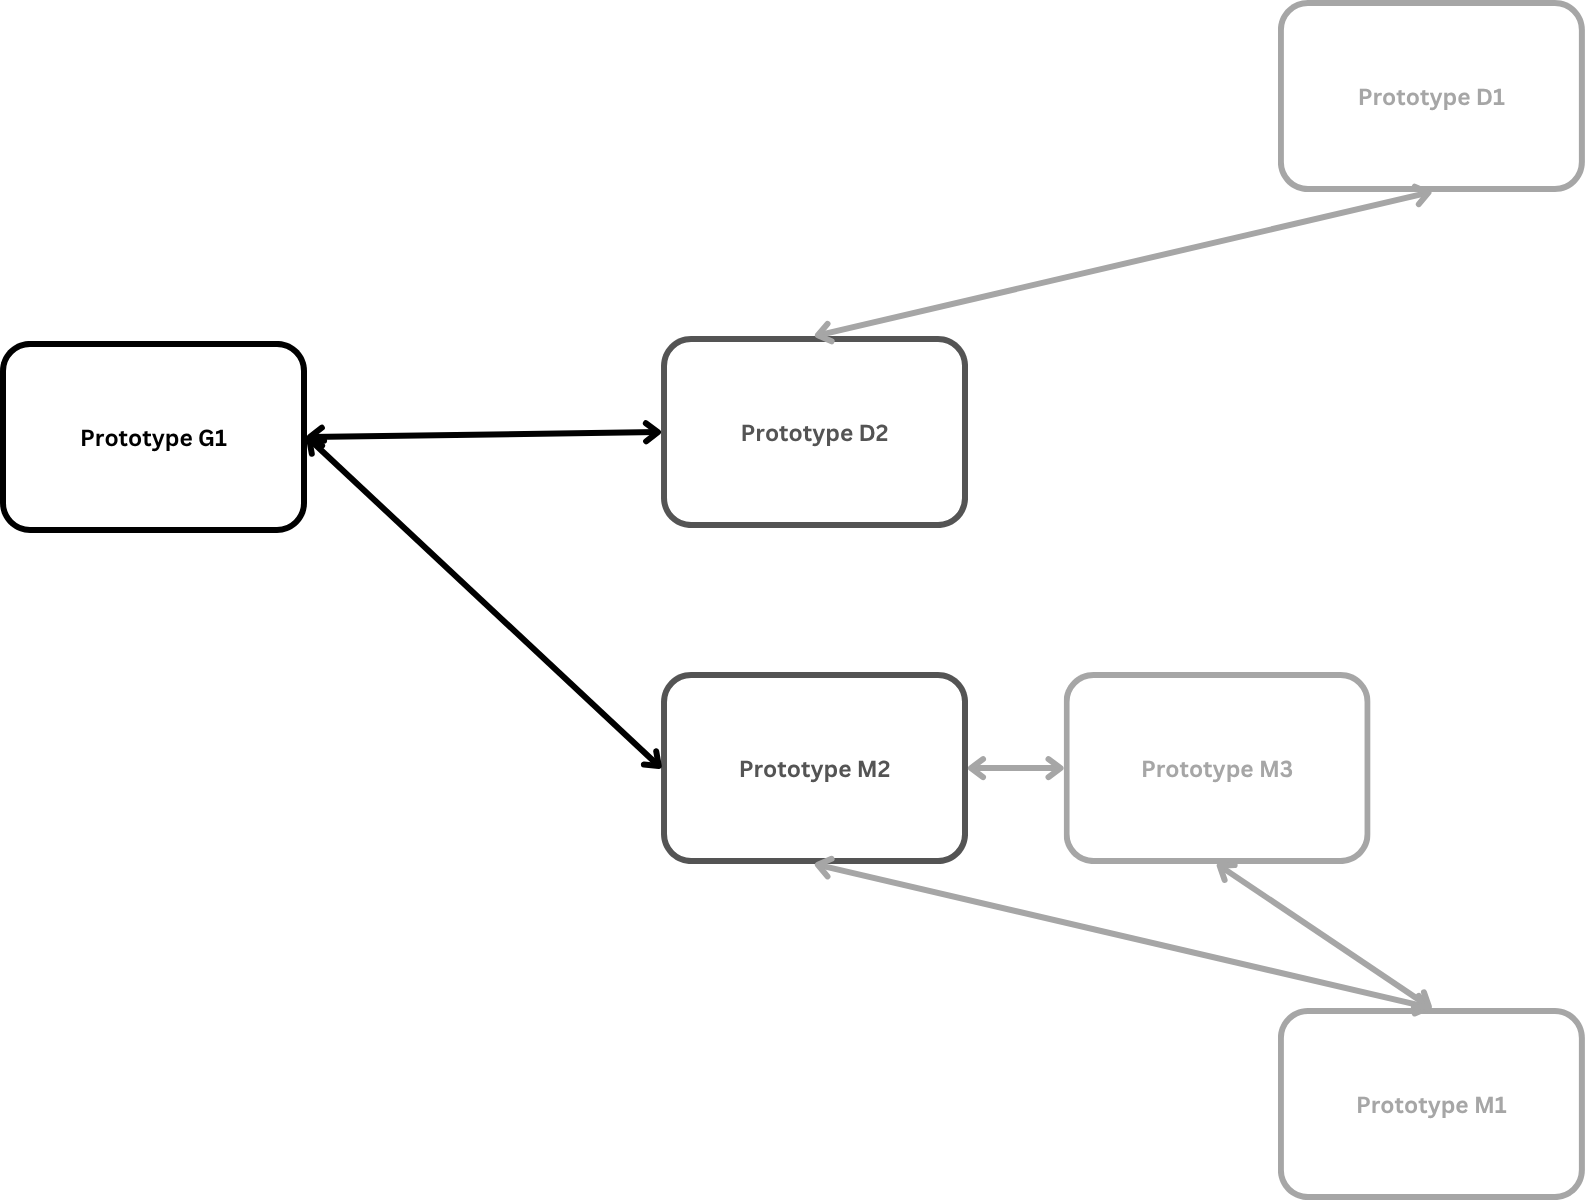
\includegraphics[width=0.7\textwidth]{figs/G-dependencies.png}
    \caption{Dependencies between prototypes of milestone 3 and the rest of the target system, shown by an interaction diagram.}
\end{figure}

\subsection{Architecture analysis}

The nature of the requirements of the milestone describe that multiple aspects shall be handled: The user may want to push their changes to either a local or remote repository. 
And the way to commit changes differs from whether the committed item is a dataset (The information of the DVC tracking file must be committed) or an \acrshort{AI} model (whole model folders can be committed from a repository within
the remote tracking server). Additionally, as versions would be defined by the commit name, a functionality to retrieve the name of the active commit could be useful.

Considering these needs and the aforementioned requirements, the conclusion reached was that the most suitable architecture for the modules of milestone 3 would mainly consist of
a monolithic application, with the possibility for it to connect momentarily to a remote repository server to push changes.

\subsection{Application type analysis}

Due to the reasons described in the previous subsection, the best option for the development of prototypes of this milestone shall be a wrapper library that encapsulates Git
operations. A library that allows to commit to local or remote repository independently on the item to be committed, facilitating thus its integration with toolkits that enable the 
tracking of datasets and models.

\subsection{Toolkit analysis}

Any API or library handling basic Git committing operations will be helpful for the development of the prototypes. Details on the final toolkit used are described in the coming subsections.

\section{Prototype design and development}

Within the coming sections, details for the design, implementation and testing phases of the development of this milestone's prototypes are shown in a sequential order. Since this milestone
is composed of a single prototype, its development will be described in the following subsection.

\subsection{Prototype \emph{G1}}

Prototype G1 is the only prototype of milestone 3, and the core dependency of many other prototypes. It has the aim of bringing basic Git operations to a library accessible to the end users.

\subsubsection{Design for prototype \emph{G1}}

The use case diagram for prototype \emph{G1} is shown in \emph{figure \ref{fig:useCaseG1}}.

\begin{figure}[H]
    \centering
    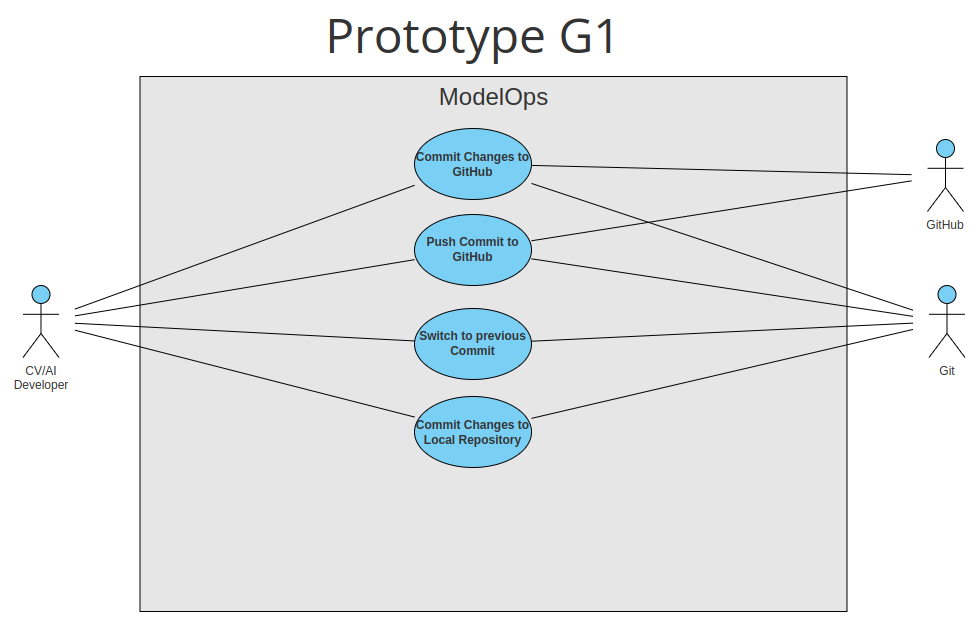
\includegraphics[width=0.7\textwidth]{figs/use-case-G1.png}
    \caption{Use case diagram for prototype \emph{G1}.}
    \label{fig:useCaseG1}
\end{figure}

Taking a look at this diagram, it is clear that there is a crucial component needed to carry out this prototype: a component that handles the Git \emph{commit} and \emph{push} operations, along with
the possible exceptions that this may generate.

\paragraph{Prototype \emph{G1} components}

\begin{itemize}
    \item \textbf{Commit Manager: }a component that will contain the functions for managing both local and remote repositories, as well as operations for chaning the active commit (\emph{checkout}).
    
    \item \textbf{Commit Exceptions: }A package that includes some special exceptions that can be raised by the Commit Manager.
\end{itemize}

\paragraph{Prototype \emph{G1} components' contents}\mbox{}\\

This paragraph will address the question of which information is stored by each of the classes and what functions will be contained within them. The methods of each component 
are described within the following lists.

\subparagraph{Commit Manager}\mbox{}\\


The attributes of this component are:

\begin{itemize}
    \item \texttt{repo\_path}: a character string that contains the path to the repository where the commits will be stored.
\end{itemize}

The methods of this component are:

\begin{itemize}
    \item \texttt{commitLocal}: processes changes over a repository to create a new version of it.
    \item \texttt{commitRemote}: processes changes over a repository to create a new version of it and push it to a remote repository.
    \item \texttt{checkoutCommit}: changes the pointer of the repository to a specific commit. The effect of this method is that the changes made to a file are temporarily 
    reverted to a previously defined state of the files within the repository. 
    \item \texttt{findCommits}: Finds the commits within a repository that have a certain name, and stores them into a map object with the dates of the commits and their UID.
    This is thought to be used for searching multiple commits within the same name in order to select to which one the user will switch to.Added in later development stages of the project due to a need encountered during the development of milestone 2.
    \item \texttt{getCurrentCommitName}: returns the active commit's name. As well as the previous method, it was developed on a later development stage to satisfy a need encountered in other milestone.
\end{itemize}

\paragraph{Prototype \emph{G1} Class Relationships}

\begin{itemize}
    \item Dependency - Commit Manager $\rightarrow$ Commit Exceptions
    \item Dependency - Commit Manager $\rightarrow$ GitPython
\end{itemize}

\paragraph{Design output}\mbox{}\\

The output design class diagram for prototype \emph{G1} is shown in \emph{figure \ref{fig:G1classDiagram}}.

\subsubsection{Implementation for prototype \emph{G1}}

This section addresses questions about the programming language used, the libraries imported and a high-level description of the implementation of the components' methods.

\paragraph{Programming language} \mbox{}\\

Given the notorious availability of tools, frameworks and libraries in the language, as well as the balance between the efectiveness easiness of use the selected language for the development
of this prototype is Python.

\paragraph{Libraries used} \mbox{}\\

The libraries used for the implementation of this prototype are:

\begin{itemize}

    \item \textbf{\emph{GitPython}: }the selected toolkit to handle \emph{commit}, \emph{push} and \emph{checkout} operations.
    \item \textbf{\emph{Logging}: }A library that enables the creation of log files and manages log operations within any Python application.
    \item \textbf{\emph{OS}: }enables interactions with the operating system, mainly used in this prototype for verifying the existence of particular files and directories.

\end{itemize}

\paragraph{Commit Manager method flows} \mbox{}\\

\textbf{Commit Manager - Constructor}
\begin{enumerate}
    \item When the function is called, the code validates the existence of a local repository on the specified path.
    \item If the repository is not found, an existing exception for non-existing repositories is raised.
    \item If the repository is found, the attribute \texttt{repo\_path} is set to the path of the repository.
    \item The function returns the instance of the class.
\end{enumerate}

\textbf{Commit Manager - commitLocal}

\begin{enumerate}
    \item Upon being called, the function checks whether the repository is dirty (there are any uncommitted changes).
    \begin{enumerate}
        \item If the repository is not dirty (nothing is to be committed), an error for such situation is raised.
    \end{enumerate}

    \item If there are uncommitted changes, the function iterates over the list of files to be added for the commit.
    \begin{enumerate}
        \item If the file is not present within the repository or is present as a directory, a warning will be left on the logs as part of the handling routine of an exception
        for such a situation.

        \item If the file is present within the repository, but it has not any uncommitted changes, it is removed from the list of files to be added for the commit as part of 
        handling an exception created for such a situation.
    \end{enumerate}

    \item Once all files have been checked, the function checks the validity of the provided commit message.
    \begin{enumerate}
        \item A commit message will be valid if it complies within the string validity standards: does not exceed length limitations, and the format passes a security check (it does not contain potential code injection substrings).
        \item If a commit message is not valid, an error for such situation is raised.
    \end{enumerate}

    \item If the commit message is valid, the function adds the files to the commit list.
    
    \item Finally, the function commits the changes to the repository.
    \begin{enumerate}
        \item Should the commit transaction fail, the error shall be processed for the user to know and then returned in a logging message.
    \end{enumerate}

    \item The function returns the number of files that were committed.
\end{enumerate}

\textbf{Commit Manager - commitRemote}
\begin{enumerate}
    \item Upon being called, the function executes the \texttt{commitLocal} method.
    \item Provided the success of the previous method call, the function pushes the changes to a remote repository.
    \begin{enumerate}
        \item Should the commit transaction fail, the error shall be processed for the user to know and then returned in a logging message.
    \end{enumerate}
    \item The function returns the number of files that were committed.
\end{enumerate}

\textbf{Commit Manager - checkoutCommit}
\begin{enumerate}
    \item Upon being called, the function checks whether the repository is dirty (there are any uncommitted changes).
    \begin{enumerate}
        \item If the repository is dirty (something is to be committed), an error for such situation is raised.
    \end{enumerate}

    \item the function checks whether the provided commit ID is valid (according to the string validity standards).
    \begin{enumerate}
        \item If the commit ID is not valid, an error for such situation is raised.
    \end{enumerate}

    \item Next, the function checks the validity of the instance number (one of the provided parameters). This instance number represents, among many commits with the same name, which one is to be checked out.
    \begin{enumerate}
        \item If the instance number is a negative number, an error for such situation is raised.
    \end{enumerate}

    \item The function checks whether there are commits with the provided name in the repository.
    \begin{enumerate}
        \item If no commits are found, an error for such situation is raised.
    \end{enumerate}

    \item If there are commits with the provided name, the function selects the commit holding the position specified by the instance parameter.
    \begin{enumerate}
        \item If the instance number is higher than the number of commits, the function selects the oldest commit with this name. On the other side, should this parameter not be specified, the latest instance will be selected.
    \end{enumerate}

    \item The function performs the checkout operation to the specified commit.

    \item The function returns the position of the selected commit within the commit list.
\end{enumerate}

\textbf{Commit Manager - findCommits}
\begin{enumerate}
    \item The function uses \emph{GitPython} to instantly retrieve the list of commits in the repository.
\end{enumerate}

\textbf{Commit Manager - getCurrentCommitName}
\begin{enumerate}
    \item The function uses \emph{GitPython} to retrieve the first line of the active commit's message.
\end{enumerate}

\subsubsection{Testing for prototype \emph{G1}}

Within the following sections, details for the testing phase of prototype \emph{G1} are shown. This includes the description of the different equivalence classes found for the prototype, and the
errors found and lessons learned during the verification of the prototype.
\newpage
\paragraph{Equivalence classes for Commit Manager}

\subparagraph{Commit Manager - Constructor} \mbox{}\\
\begin{enumerate}
    \item \texttt{repo\_path} exists, is a directory and contains a local repository.
    \item \texttt{repo\_path} is not a valid Local Repository.
\end{enumerate}

\subparagraph{Commit Manager - commitLocal} \mbox{}\\
\begin{enumerate}
    \item The list of files to commit is not empty and the commit message is valid.
    \item The repository to commit is not dirty.
    \item The list of files to commit is empty.
    \item The commit message is not valid.
    \item After checking file validity, the list of files to commit is empty.
\end{enumerate}

\subparagraph{Commit Manager - checkoutCommit} \mbox{}\\
\begin{enumerate}
    \item All parameters are valid.
    \item The commit ID is not valid.
    \item The list of commits with the requested name is empty.
    \item instance number is greater than the number of found commits.
    \item instance number is negative.
\end{enumerate}

\paragraph{Test suites for Commit Manager}\mbox{}\\

The test suites for this class can be found in \emph{annex reference placeholder}. % Referencia al Anexo con las tablas (porque pueden ser muy grandes y no es plan). Esto no es prioritario, puede esperar

\paragraph{Errors found and lessons learned}\mbox{}\\

The errors encountered during the course of the testing phase of prototype \emph{G1} are shown in \emph{annex reference placeholder}. % De nuevo, esto puede esperar porque va al anexo


\chapter{Dataset configuration management in MADTrack}\label{cap:Milestone1}

This chapter will cover the development of the features described in milestone 1 (codename \emph{D}), which is focused on the development of features related to Dataset
Configuration Management. This module will work in conjuction with the general configuration management module (see \emph{chapter \ref{cap:Milestone3}}) to provide mechianisms
to track and control the changes of the biggest of files. This chapter will introduce the main issues and address the problems to solve to achieve the goals defined for this
milestone.

\section{Introduction}

One of the partial objectives defined for this Final Degree Project involves the development of a module for tracking and versioning datasets. These datasets can be of variable
size, but in many cases bigger than what a free-of-charge configuration management platform can handle. The lack of the existence of a platform that can handle such issue at
at a feasible cost motivates the creation of this dataset tracking module. The main focus of the prototypes of milestone 1 is to provide a mechanism for tracking changes within
datasets, without the need of committing them to the configuration management platform. Another issue to be tackled is that of bringing the correct dataset to the correct environment,
providing at least an interface for this purpose. Firstly, an analysis for the requirements defined for this milestone will be made, separating them by the most suitable
prototypes to be developed, to then proceed to the development details of each of these.

\section{Requirements analysis for milestone 1}

Analysis has the purpose of defining the high-level outline of the application. The definition of this outline requires addressing the question of the most suitable architecture and
application type for the prototypes of this milestone. This analysis will also define the characteristics of a tookit suitable for their development. Furthermore, the
protocol for versioning datasets will also be defined within the analysis phase.

\subsection{Requirements involved}

The requirements involved within this milestone have already been listed within \emph{table \ref{tab:requirementsMilestone1}}. Since this requirements are contained within different prototypes,
it is particularly convenient to define which requirements belong to which prototype. The final requirement division is defined within \emph{table \ref{tab:requirementsD1}} and \emph{table \ref{tab:requirementsD2}}.

Apart from the final requirement division for each prototype, all prototypes must satisfy the non-functional requirements listed within \emph{table \ref{tab:nonFunctionalRequirements}}.

\begin{table}[H]
    \centering
    \begin{tabular}{ | c | p{9cm} | p{3cm} |}
        \hline
        \textbf{Requirement ID} & \textbf{Requirement Description} & \textbf{priority (MoSCoW)} \\ \hline
        DFR1.2   & The system MUST keep track of the routes where models and datasets are stored    & Must have\\ \hline
    \end{tabular}
    \caption{Requirements for prototype \emph{D1}}
    \label{tab:requirementsD1}
\end{table}

\begin{table}[H]
    \centering
    \begin{tabular}{ | c | p{9cm} | p{3cm} |}
        \hline
        \textbf{Requirement ID} & \textbf{Requirement Description} & \textbf{priority (MoSCoW)} \\ \hline
		DFR1     & The system MUST keep ordered track of dataset configurations.                    & Must have\\ \hline
		DFR1.1   & The system MUST detect changes in the size (rows and columns) of datasets.       & Must have\\ \hline
    \end{tabular}
    \caption{Requirements for prototype \emph{D2}}
    \label{tab:requirementsD2}
\end{table}

\subsection{Integration with the rest of the system}

Prototypes within milestone 1 only have meaningful interaction with the general configuration management module, mainly because of their dependency from the committing and
checkout methods from milestone 3. 

\begin{figure}[H]
    \centering
    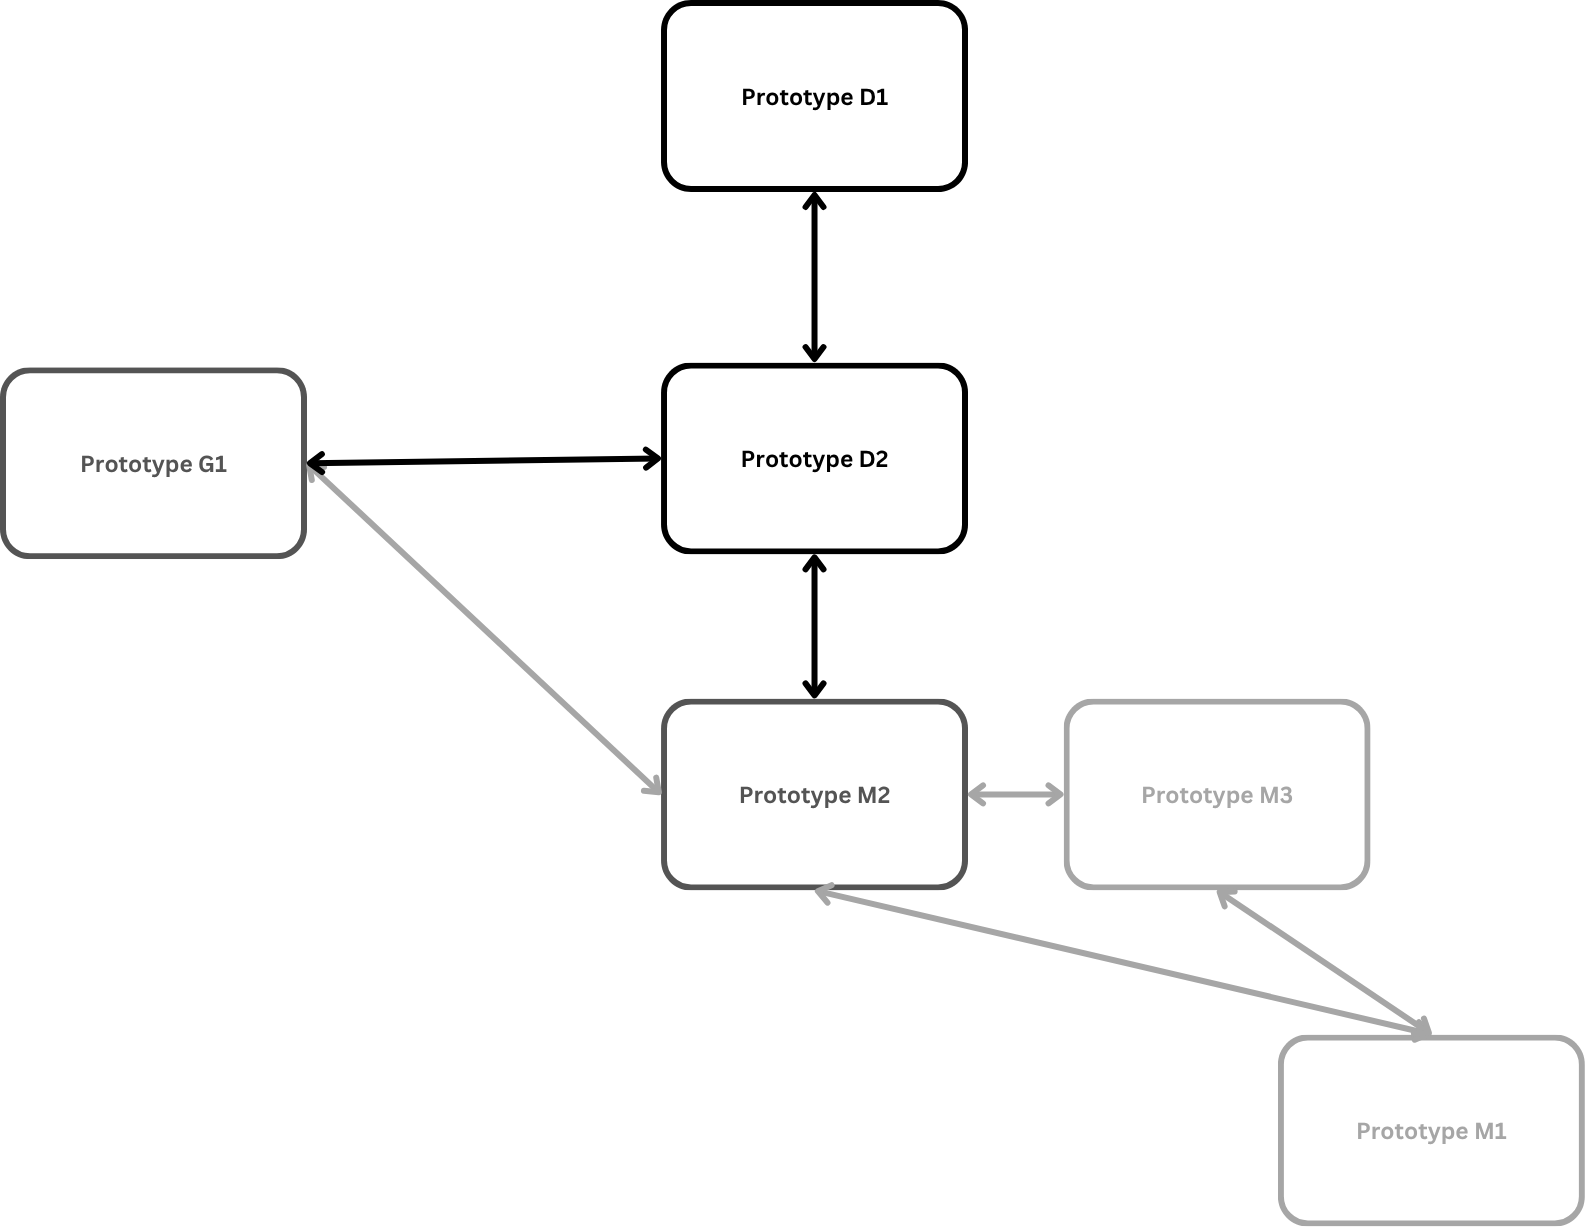
\includegraphics[width=0.7\textwidth]{figs/D-dependencies.png}
    \caption{Dependencies between prototypes of milestone 1 and the rest of the target system, shown by an interaction diagram.}
\end{figure}

\subsection{Architecture analysis}

The requirements describe the need for users to be able to locate files regarding datasets (and models, if it were necessary). Hence, an heterogeneous system will be 
required that is able to load a file or dataset from some sort of initial information, such as an URL. The architecture of this application will be monolithic, but will 
also have the capability to handle connections to remote file systems. Also, the coming prototypes will integrate an automatic version detection system that loads the file and 
sets it in the correct version.

\subsection{Application type analysis}

Since the main objective of this prototype is to locate and load files and perform configuration management operations on them, the most suitable application type is a Wrapper Library 
that covers online and local operations from a machine with authorized access to the file system.

\subsection{Toolkit analysis}

The most suitable toolkits that may serve for the development of this prototype are those related to dataset configuration management (from \emph{Chapter \ref{cap:StateOfTheArt}},
the tool with the most potential was DVC), a toolkit for accessing remote file systems securely and locating files within the local machine, and any toolkit providing a 
mechanism for changing between file versions (the Commit Manager component from prototype \emph{G1} of the system can be used for this purpose).

\subsection{Versioning protocol for datasets}\label{sec:versioningProtocol}

Any dataset integrated within MADTrack will be versioned using the following naming system:

\begin{table}[H]
    \centering
    \begin{tabular}{|c|}
        \hline
        \texttt{<dataset\_name> v<major\_version>.<minor\_version>} \\ \hline
    \end{tabular}
\end{table}

where:

\begin{itemize}
    \item \texttt{<dataset\_name>} is the name of the dataset.
    \item \texttt{<major\_version>} is a positive integer that represents major changes within the datasets without breaking semantics on the purpose of the dataset.
    \item \texttt{<minor\_version>} is a positive integer that represents minor changes within the datasets.
\end{itemize}

\section{Prototype design and development}

Within the coming sections, details for the design, implementation and testing phases of the development of this milestone's prototypes are shown in a sequential order. This
milestone is composed of two prototypes, whose development details will be shown in the following subsections.

\subsection{Prototype \emph{D1}}

Prototype D1 consists in the initial stage of development of milestone 1. The objective of this prototype is to 
provide the necessary mechanisms to integrate and transparently locate a dataset within the target system.

\subsubsection{Design for prototype \emph{D1}}

The use case diagram for prototype \emph{D1} is shown in \emph{figure \ref{fig:useCaseD1}}.

\begin{figure}[H]
    \centering
    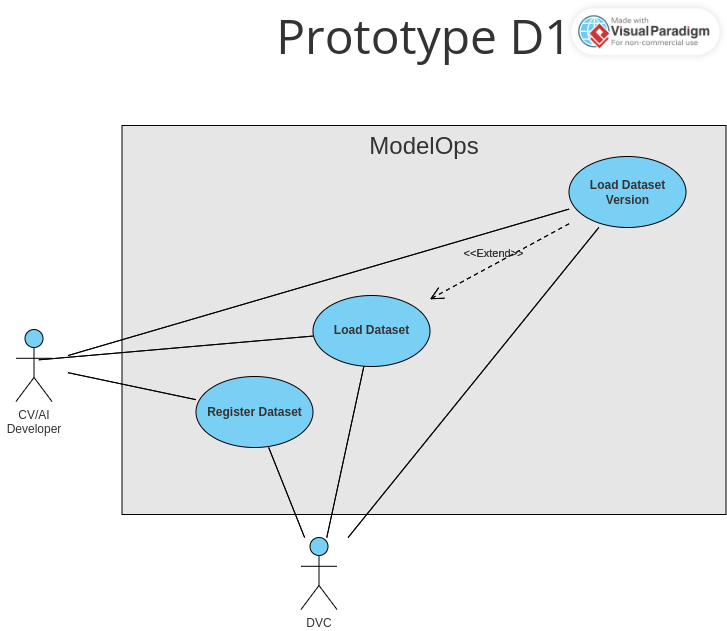
\includegraphics[width=0.7\linewidth]{figs/use-case-D1.png}
    \caption{Use case diagram for prototype \emph{D1}.}
    \label{fig:useCaseD1}
\end{figure}

Two main tasks can be extracted from this use case diagram. The first task is related to the tracking of changes within datasets, focusing particularly on enabling this action on a 
dataset. The second task, additionally, is to enable users to load datasets in either their latest version or any specific existent version. For the fulfillment of 
this objective, two new components will be created, along with a pack of classes to represent exceptions, errors and specific states for a dataset repository.

\paragraph{Prototype \emph{D1} components}

\begin{itemize}
    \item \textbf{Dataset Tracker: }this component will be used for carrying out tasks related with tracking changes on the datasets. For this prototype, it should be 
    capable of starting the change tracking on a dataset and revert its state to a previous, past version.
    
    \item \textbf{Integration States: }an enumeration component that contains the possible states of integration of a dataset repository into ModelOps' configuration management 
    system: Fully integrated, partially or semi integrated or not integrated.
    
    \item \textbf{Dataset Fetchers: }a series of components with the main purpose of providing users with the mechanism to obtain datasets from virtually any location, as well as to 
    load them in their different versions, by means of a unified interface to name the dataset versions. For this prototype, only one implementation of this interface will be made.
    
    \item \textbf{Dataset Exceptions: }a set of exceptions and errors created to represent the possible undesireable or exceptional states that can be encountered by operating 
    the previous two components.

\end{itemize}



\paragraph{Prototype \emph{D1} design output}\mbox{}\\

The design for prototype \emph{D1} is shown in \emph{Placeholder for annex figure}.

\subsubsection{Implementation for prototype \emph{D1}}

On the coming paragraphs, details for the tools used to implement this prototype are revealed.

\paragraph{Libraries} \mbox{}\\

The libraries used for the implementation of this prototype were:

\begin{itemize}
    \item \textbf{\emph{GitPython}: }this toolkit also helped in this prototype, as the Commit Manager has a synergy with the dataset configuration management module.
    \item \textbf{\emph{DVC}: }this library was used to implement the dataset integration and version change functionalities.
    \item \textbf{\emph{Logging}: }A library that enables the creation of log files and manages log operations within any Python application.
    \item \textbf{\emph{OS}: }this library returns for providing repository existence verification mechanisms.
    \item \textbf{\emph{SHutil}: }a library that enables the creation and removal of directories and files. mainly used for developing functionalities for the Local Dataset Fetcher component.
\end{itemize}

\subsubsection{Testing for prototype \emph{D1}}

This subsection contains information on the test suites and errors encountered during the testing phase of the prototype.

\paragraph{Test suites for prototype \emph{D1}}\mbox{}\\

The test suites for this class can be found in \emph{annex reference placeholder}. % Referencia al Anexo con las tablas (porque pueden ser muy grandes y no es plan). Esto no es prioritario, puede esperar

\paragraph{Errors found and lessons learned during the development of prototype \emph{D1}}\mbox{}\\

The errors encountered during the course of the testing phase of prototype \emph{G1} are shown in \emph{annex reference placeholder}. % De nuevo, esto puede esperar porque va al anexo

\subsection{Prototype \emph{D2}}

Prototype D2 is the second stage of development of Milestone 1. The objective of this prototype is to provide the necessary mechanisms to commit changes to a dataset.

\subsubsection{Design for prototype \emph{D2}}

The output of the design for prototype \emph{D2} is developed by designating the various components that make up this prototype, their contents and their connection with the rest of the system.
Hence, the design details for this prototype are shown in the following paragraphs.

\paragraph{Components for prototype \emph{D2}} \mbox{}\\

The use case diagram is shown in \emph{figure \ref{fig:useCaseD2}}.

\begin{figure}[H]
    \centering
    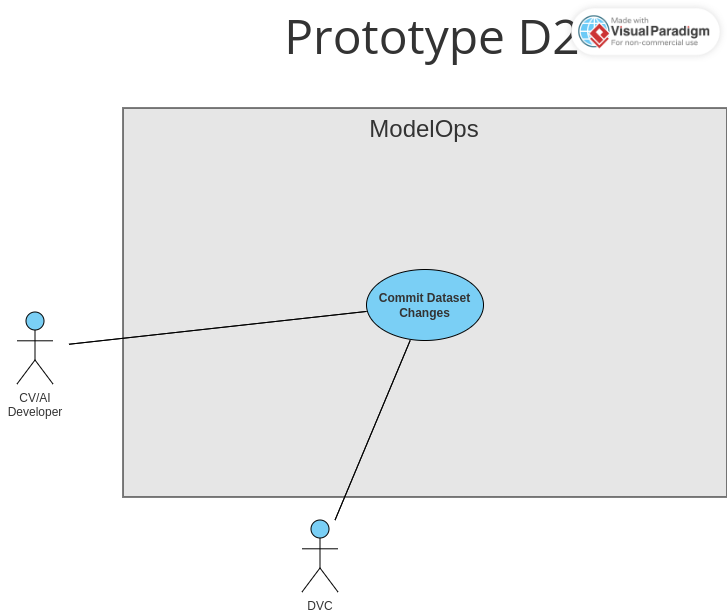
\includegraphics[width=0.7\linewidth]{figs/use-case-D2.png}
    \caption{Use case diagram for prototype \emph{D2}.}
    \label{fig:useCaseD2}
\end{figure}

The main task is to perform commits over a dataset. For this objective, the Dataset Tracker component can be used, as it already has a function that allows the user to 
commit changes to a dataset and generate a new version of it. Hence, the involved components are:

\begin{itemize}
    \item \textbf{Dataset Tracker: }this class will be used for carrying out tasks related with tracking changes on the datasets. For this prototype, it should be capable of creating new versions of a dataset and upload them to a local or remote repository.
\end{itemize}

\paragraph{Design output for prototype \emph{D2}}\mbox{}\\

The design class diagram for prototype D2 is shown in \emph{Placeholder for annex figure}.

\subsubsection{Implementation for prototype \emph{D2}}

Prototype \emph{D2} mostly follows the same implementation details as the previous prototype of the milestone. Following Python as the main programming language and the same
libraries.

\subsubsection{Testing for prototype \emph{D2}}

The testing phase of prototype \emph{D2} was clearly focused on testing the new methods. Since the method \texttt{getCurrentDatasetName} is a read-only 
method that just calls the Commit Manager, its testing can be ommitted. The test suites of the remaining method can be found at \emph{annex reference placeholder} and the errors fixed can be found at \emph{annex reference placeholder}.

\paragraph{Test suites for prototype \emph{D2}}\mbox{}\\

The test suites for this class can be found in \emph{annex reference placeholder}.

\paragraph{Errors found and lessons learned during the development of prototype \emph{D2}}\mbox{}\\

The errors encountered during the course of the testing phase of prototype \emph{D2} are shown in \emph{annex reference placeholder}.


\chapter{Model Configuration Management in MADTrack}\label{cap:Milestone2}

This chapter covers the development of milestone 2 (codename \emph{M}), related to the development of features for configuration
management applied to \acrshort{AI} models. This module will provide great value to the end user, increasing the reproducibility of the
training performed on a given model. For these reasons, this is the chapter with the most prototypes to be developed, and the one with 
the most complex architecture.

\section{Introduction}

This chapter aims to provide the necessary documentation of the development of the requirements and features necessary for the fulfillment
of one of the partial objectives of the project, which consists in developing a module for versioning \acrshort{AI} models. This module will
integrate a vital component for deployment, the MADTrack Tracking Server, which will handle the requests from users and store the training 
configurations. This component, along with the developed solution for the target system that will be used to register the trainings, will ensure
every single training is accessible to the users, and can be reproduced with similar results in the future.

\section{Requirements analysis for milestone 2}

Just as with the other milestones, an analysis of the requirements will be performed to define a high-level outline of what is to come on the 
following sections. First, the requirements will be grouped semantically according to the milestone 1 prototype that best suits for each requirement,
and then make a study of what application type and architecture is more suitable for the module, and what toolkits out of the ones explored in 
\emph{Chapter \ref{cap:StateOfTheArt}} would be the most helpful to develop the prototype.

\subsection{Requirements involved}

Just like milestone 1, milestone 2 has a set of requirements that have to be semantically divided into the different prototypes. The requirements belonging
to milestone 2 (those with the prefix \emph{MFR}) have been already listed within \emph{table \ref{tab:functionalRequirements}}, and now they will be divided
into three prototypes: \emph{M1} (requirement listed within \emph{table \ref{tab:requirementsM1}}), \emph{M2} (requirement listed within \emph{table \ref{tab:requirementsM2}}),
and \emph{M3} (requirement listed within \emph{table \ref{tab:requirementsM3}}).

\begin{table}[H]
    \centering
    \begin{tabular}{ | c | p{9cm} | p{3cm} |}
        \hline
        \textbf{Requirement ID} & \textbf{Requirement Description} & \textbf{priority (MoSCoW)} \\ \hline
        MFR1     & The system MUST handle the concept of experiments. & Must have \\ \hline
        MFR1.1   & The system MUST identify an experiment by its identification string, or ID. & Must have \\ \hline
        MFR1.2   & The system MUST provide a mechanism for creating experiments. & Must have \\ \hline
        MFR1.3   & The system MUST not accept an experiment creation request that has no experiment name. & Must have \\ \hline
        MFR1.4   & The system MUST separate commits from different experiments. & Must have \\ \hline
        MFR1.5   & The system MUST provide a mechanism for deleting experiments. & Must have \\ \hline
        MFR1.6   & The system MUST provide a mechanism for switching between experiments. & Must have \\ \hline
    \end{tabular}
    \caption{Requirements for prototype \emph{M1}.}
    \label{tab:requirementsM1}
\end{table}

\begin{table}[H]
    \centering
    \begin{tabular}{ | c | p{9cm} | p{3cm} |}
        \hline
        \textbf{Requirement ID} & \textbf{Requirement Description} & \textbf{priority (MoSCoW)} \\ \hline
        MFR2     & The system MUST keep ordered track of machine learning model configurations. & Must have \\ \hline
        MFR2.1   & The system MUST track which dataset was used to train the model. & Must have \\ \hline
        MFR2.2   & The system MUST track which dataset was used to validate the model. & Must have \\ \hline
        MFR2.3   & The system MUST track which dataset was used to test the model. & Must have \\ \hline
        MFR2.4   & The system MUST track the code used for programming the model's training. & Must have \\ \hline
        MFR2.5   & The system MUST track the configuration of the model's hyperparameters and random parameters used in the training of an AI model. & Must have \\ \hline
        MFR2.6   & The system MUST track the metrics achieved by an AI model. & Must have \\ \hline
        MFR2.7   & The system MUST provide users with a mechanism to mark an AI model as currently deployed. & Should have \\ \hline
        MFR2.8   & The system MUST keep track of the additional parameters used by an AI model if it handles domain-specific data. This will be tested for the domain of Earth Observation. & Must have \\ \hline
    \end{tabular}
    \caption{Requirements for prototype \emph{M2}.}
    \label{tab:requirementsM2}
\end{table}

\begin{table}[H]
    \centering
    \begin{tabular}{ | c | p{9cm} | p{3cm} |}
        \hline
        \textbf{Requirement ID} & \textbf{Requirement Description} & \textbf{priority (MoSCoW)} \\ \hline
        MFR3     & The system MUST provide a mechanism for evaluating an AI model's metrics' goodness. & Should have \\ \hline
        MFR3.1   & The system MUST provide a mechanism for choosing policies to evaluate an AI model's metrics' goodness. & Should have \\ \hline
        MFR3.2   & The system MUST provide a mechanism for identifying the experiment or model with the best values on the chosen metrics. & Should have \\ \hline
        MFR3.3   & The system SHOULD order the model trainings made on an experiment by the goodness of the values on the chosen metrics. & Should have \\ \hline
        MFR4     & The system MUST provide a mechanism for visualizing the performance report for a trained AI model (if any). & Should have \\ \hline
        MFR5     & The system MUST provide a mechanism to visualize the training graph of a model (this is, the graph that describes the progress of the metrics of a model after each epoch). & Could have \\ \hline
    \end{tabular}
    \caption{Requirements for prototype \emph{M3}.}
    \label{tab:requirementsM3}
\end{table}

\subsection{Integration with the rest of the system}

Prototypes within milestone 2 have a strong relation with the rest of milestones, since they need the configuration management mechanisms to commit changes made to the folders that track
the model training configurations, and will also use the dataset versioning system on dataset logging tasks.

\begin{figure}[H]
    \centering
    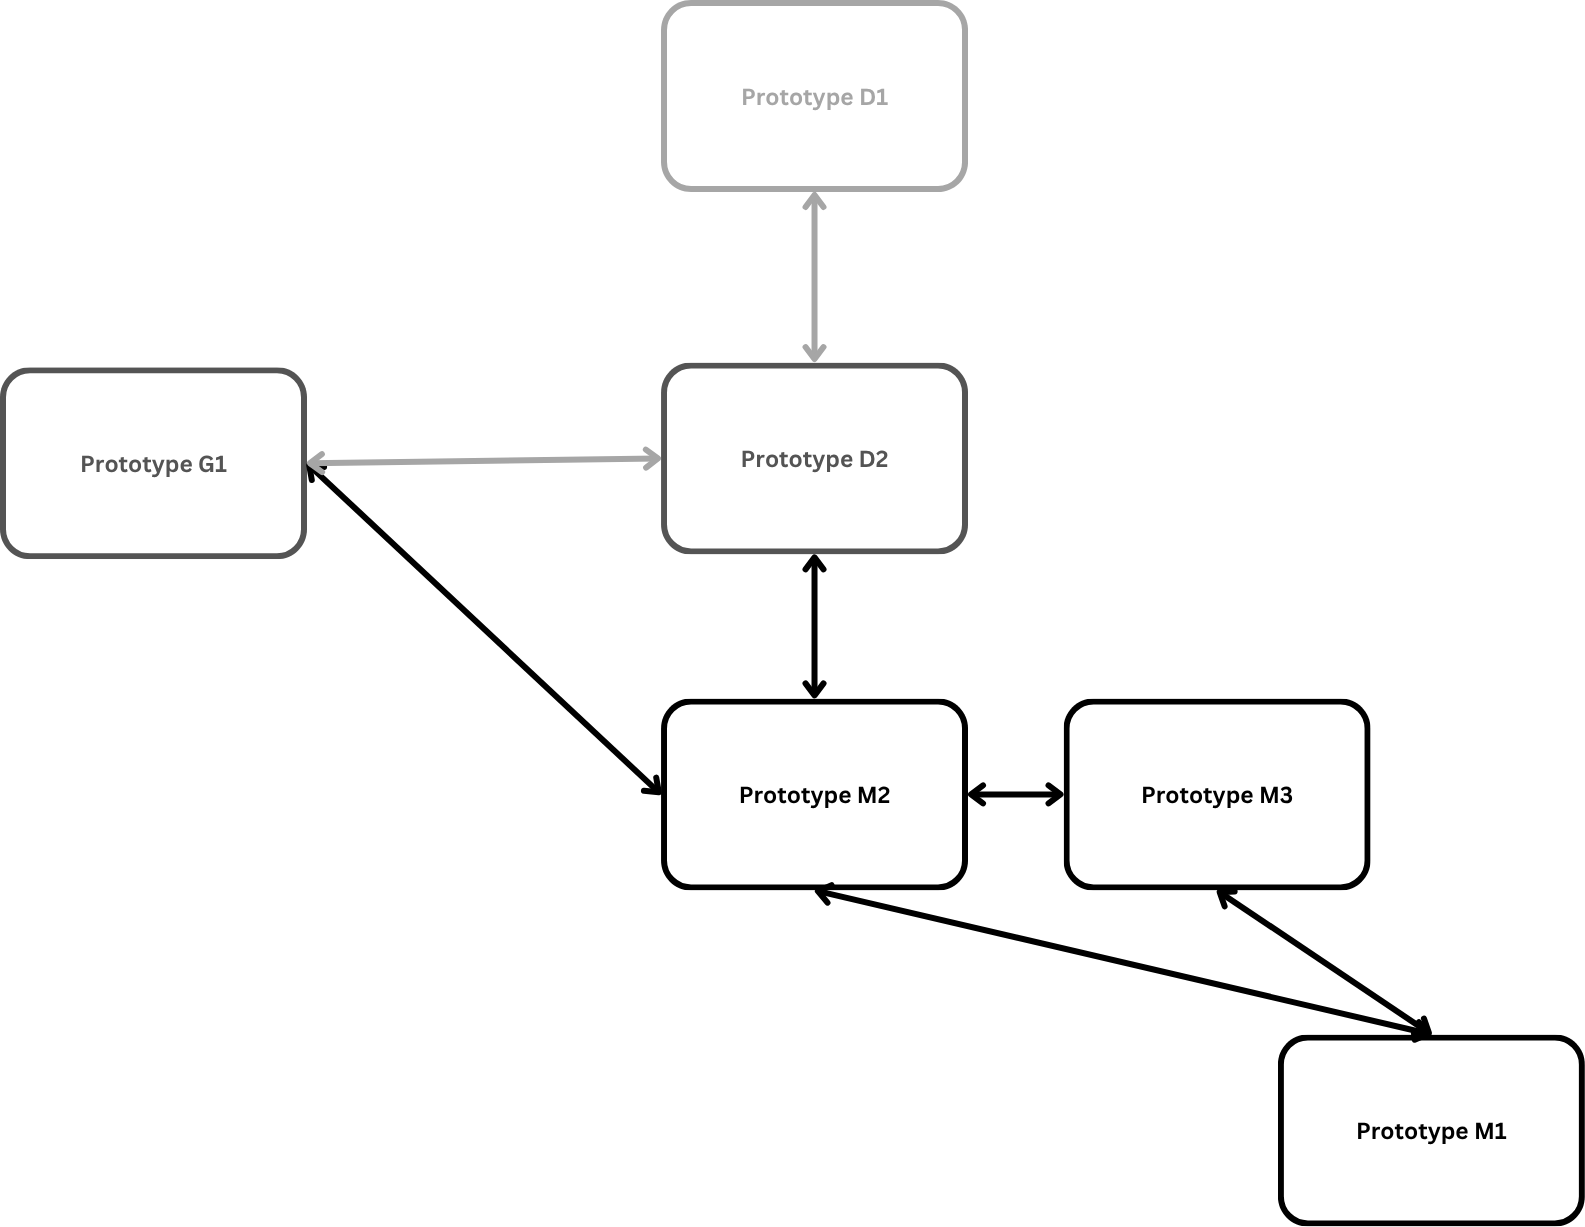
\includegraphics[width=0.7\textwidth]{figs/M-dependencies.png}
    \caption{Dependencies between prototypes of milestone 2 and the rest of the target system, shown by an interaction diagram.}
\end{figure}

\subsection{Architecture analysis}

The main objective of the milestone is to enable the target system to handle experiments, model trainings, register and version them. The need for
registration of events happening on a machine at the time they are happening creates the need for a component that can manage all of them. This component
shall be separate from the rest of the system so as to increase portability. Hence, the architecture of this module will be distributed, with two main components.

\subsection{Application type analysis}

The aim of this prototype is to manage the existence of experiments. Since this is a two-sided task, the best approach is to provide the 
management functionality inside a Wrapper Library, from which the user will be able to create, delete and switch their active experiment, as well
as managing their model trainings using code, while a remote tracking server will be in charge of processing these requests with a web 
application, provided by an external toolkit.

\subsection{Toolkit analysis}

The most suitable toolkit for the development of this milestone is the one that provides a mechanism for creating experiments under the 
definition of a series of \acrshort{AI} model lifecycles performed with the purpose to achieve a suitable model for a specific goal. A good example is MLFlow
(overviewed in \emph{Chapter \ref{cap:StateOfTheArt}}), which is a tool for model registration and experiment tracking.

\section{Prototype design and development}

The following subsections contain details about the design, implementation and teting process for the three prototypes this milestone is composed of.

\subsection{Prototype \emph{M1}}

Prototype \emph{M1} is the first stage of development of Milestone 2 (consisting in \acrshort{AI} model versioning and tracking). The objective of this prototype is to provide 
the necessary mechanisms to register experiments into a remote server, based on their purpose.

\subsubsection{Design for prototype \emph{M1}}

The following sections describe the design process of prototype \emph{M1}.

\paragraph{Components for prototype \emph{M1}} \mbox{}\\

The use case diagram which summarizes this prototype's needs is shown in \emph{figure \ref{fig:useCaseM1}}.

\begin{figure}[H]
    \centering
    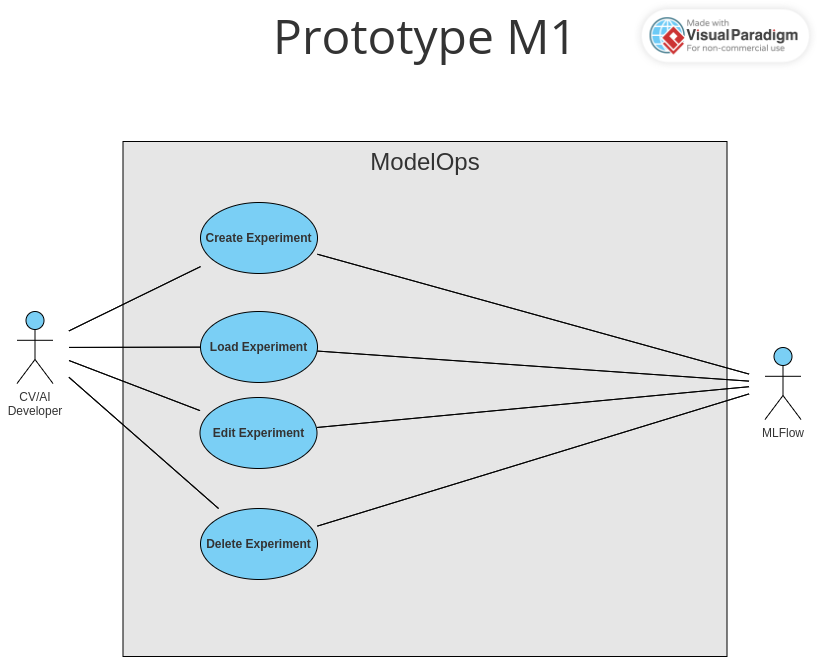
\includegraphics[width=0.7\linewidth]{figs/use-case-M1.png}
    \caption{Use case diagram for prototype \emph{M1}.}
    \label{fig:useCaseM1}
\end{figure}

The objective of this prototype is to handle the lifecycle of experiments: creation, switching,
edition and deletion. For this purpose, a new class with the role of managing this life cycle will be created, along with a new component which 
will relate to deployment:

\begin{itemize}
    \item \textbf{Experiment Manager: }this class will have the role of managing the life cycle of experiments, covering all the aforementioned 
    operations. It will be able to create, switch, edit and delete experiments.

    \item \textbf{Tracking Server: }a distributed component consisting on a docker container, running locally for the meantime, which will contain
    the Active MADTrack Tracking server which will use a file system as storage.

    \item \textbf{Model Tracking Exceptions }: a package that includes some special exceptions that can be raised by the Experiment Manager. 
\end{itemize}

\paragraph{Design output for prototype \emph{M1}}\mbox{}\\

The design class diagram for prototype \emph{M1} is shown in \emph{Placeholder for annex figure}.

\subsubsection{Implementation for prototype \emph{M1}}

The following lines describe the details of the implementation of the prototype.

\paragraph{Libraries} \mbox{}\\

The libraries used for this implementation are:

\begin{itemize}
    \item \textbf{MLFlow: }an open-source Python library that provides a unified API for tracking and logging machine learning experiments.
    \item \textbf{Logging: }a library that enables the creation of log files and manages log operations within any Python application.
    \item \textbf{OS: }a Python library enabling operating system interaction. It will be used to build the necessary paths to local file repositories.
    \item \textbf{YAML: }A Python library that provides a way to represent data in YAML format using simple structures.
\end{itemize}

\subsubsection{Testing for prototype \emph{M1}}

The following paragraphs contain information about the test suites and errors fixed during the testing process of prototype \emph{M1}.

The test suites for this prototypes can be found in \emph{annex reference placeholder}. % Referencia al Anexo con las tablas (porque pueden ser muy grandes y no es plan). Esto no es prioritario, puede esperar
In the same way, errors encountered during the course of the testing phase of prototype \emph{M1} are shown in \emph{annex reference placeholder}. % De nuevo, esto puede esperar porque va al anexo

\subsection{Prototype \emph{M2}}

Prototype \emph{M2} is the second stage of development of milestone 2. This prototype will focus on effective \acrshort{AI} logging during the model lifecycle. 
This objective can be accomplished by providing mechanisms for logging all 
the datasets (test, train, validation), the code used to train the model, the hyperparameters, and domain-specific data.

\subsubsection{Design for prototype \emph{M2}}

The following sections describe the design process of prototype \emph{M2}.

\paragraph{Components for prototype \emph{M2}} \mbox{}\\

First, it is necessary to look at the use case diagram, (shown at \emph{figure \ref{fig:useCaseM2}}), which summarizes this prototype's needs.

\begin{figure}[H]
    \centering
    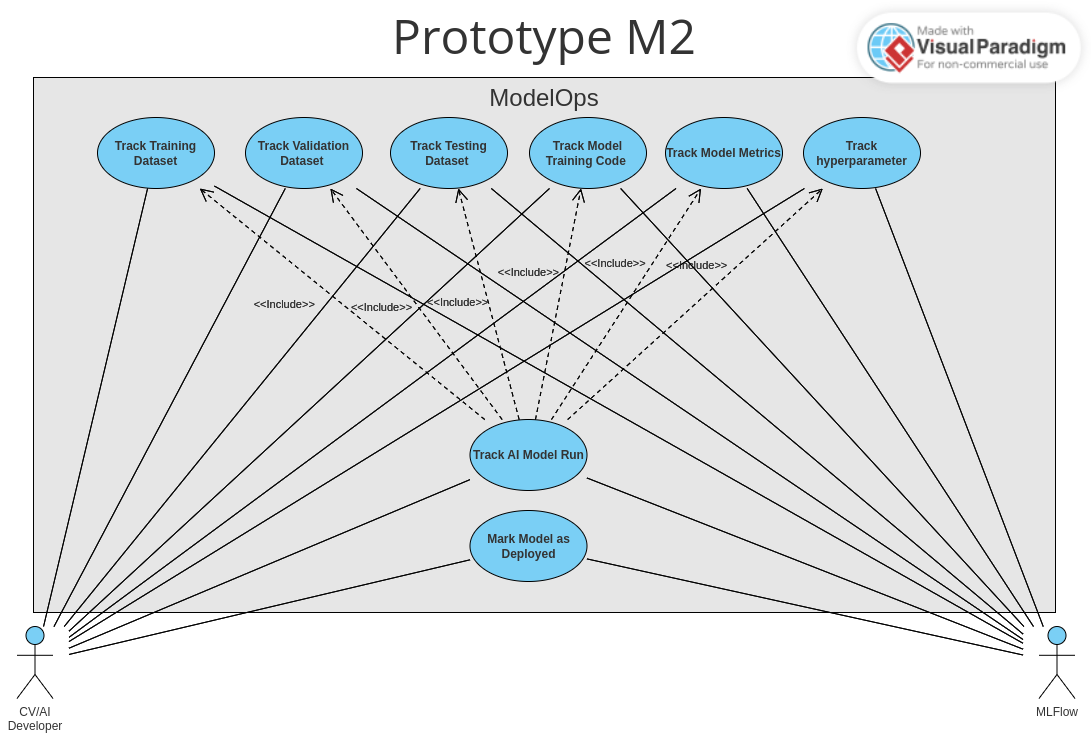
\includegraphics[width=0.7\linewidth]{figs/use-case-M2.png}
    \caption{Use case diagram for prototype \emph{M2}.}
    \label{fig:useCaseM2}
\end{figure}

The objective of this prototype is to enable users to fill their experiments with \emph{Model Runs} (for more information about these, please refer to
\emph{section \ref{sec:mlflow}}), which will have several data logged according to the needs of the user. For this objective, a new component will be responsible 
of representing an \acrshort{AI} model run, along with changes in the Experiment Manager component. The list of components involved in this prototype is:

\begin{itemize}
    \item \textbf{Model Run:} This component will be in charge of representing a run of a single model within the training workflow. Its main functionality
    resides in the component's capability of logging the necessary items to store the configuration of a run.

    \item \textbf{Experiment Manager: }This class will have new functionalities, such as the capability to run a complete run workflow or to register a new \acrshort{AI} 
    model version within the model registry.

    \item \textbf{Tracking Server: }This component will be able to store the necessary data to enable logging in the model run. The details about its architecture are revealed in \emph{Chapter }
\end{itemize}

\paragraph{Design output for prototype \emph{M2}}\mbox{}\\

The design class diagram for prototype M2 is shown in \emph{Placeholder for annex figure}.

\subsubsection{Implementation for prototype \emph{M2}}

This are the lines that contain the main details about this prototypes implementation. The main libraries do not differ from
the previous prototype.

\subsubsection{Testing for prototype \emph{M2}}

The particularity of the testing of this prototype is that it could be mostly done from the Experiment Manager component, since it has a method that calls the methods
from the Model Run component. The test suites of the Experiment Manager will also test the Model Run component.

\paragraph{Test suites for prototype \emph{M2}}\mbox{}\\

The test suites for this class can be found in \emph{annex reference placeholder}.

\paragraph{Errors found and lessons learned}\mbox{}\\

The errors encountered during the course of the testing phase of prototype \emph{M2} are shown in \emph{annex reference placeholder}.

\subsection{Prototype \emph{M3}}

Prototype M3 is the third stage of development of Milestone M (AI model versioning and tracking). This prototype will be focused on how metrics are shown in the
MADTrack system and how they are presented to end users, as well as the final presentation of these metrics on a performance report (which would be logged as 
another parameter and printed out when completing a Model Run, if necessary).

\subsubsection{Design for prototype \emph{M3}}

The following sections describe the design process of prototype \emph{M3}.

\paragraph{Components for prototype \emph{M3}} \mbox{}\\

The use case diagram is shown in \emph{figure \ref{fig:useCaseM3}}, summarizing thus the needs of this prototype.

\begin{figure}[H]
    \centering
    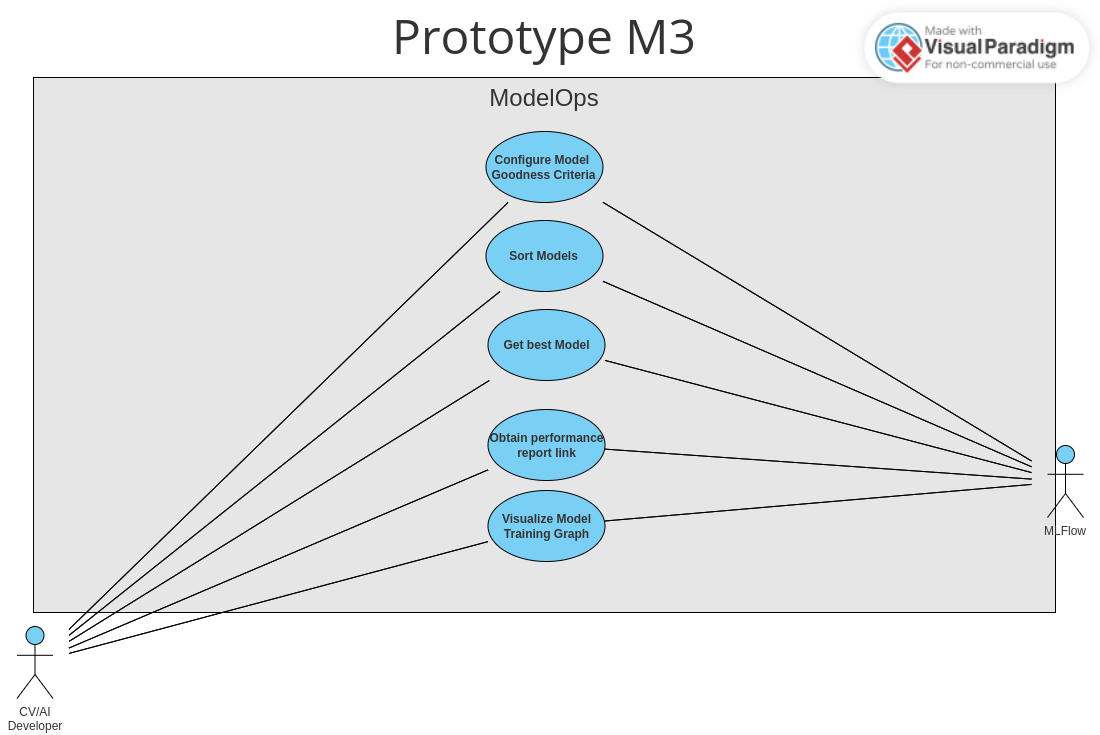
\includegraphics[width=0.7\linewidth]{figs/use-case-M3.png}
    \caption{Use case diagram for prototype \emph{M3}.}
    \label{fig:useCaseM3}
\end{figure}

The objective of this prototype is to enable users to extend the functionality of a model run, allowing the goodness of the metrics can be configurable, which in turn enables the 
model runs can be sorted according to a specific metric. This means that the best model run can finally be highlighted in some way. Additionally, the system will also provide a 
mechanism to log a performance report for the model, which will be stored as an artifact of the model run and access to it will also be provided in the logs, and the system will also provide a way to 
visualize the training graph of the model, if it is trained.

For this reason, the main component involved within this prototype is the Model Run component, which will gain additional methods, and the Experiment Manager component.

\paragraph{Design output for prototype \emph{M3}}\mbox{}\\

The design class diagram for prototype M3 is shown in \emph{Placeholder for annex figure}.

\subsubsection{Implementation for prototype \emph{M3}}

The following sections describe the implementation process of prototype \emph{M3}. The language and the libraries used are the same as for the other prototypes of this milestone.

\subsubsection{Testing for prototype \emph{M3}}

The main testing methods focus on the new methods of the Model Run component.

\paragraph{Test suites for prototype \emph{M3}}\mbox{}\\

The test suites for this class can be found in \emph{annex reference placeholder}.

\paragraph{Errors found and lessons learned during the development of prototype \emph{M3}}\mbox{}\\

The errors encountered during the course of the testing phase of prototype \emph{M3} are shown in \emph{annex reference placeholder}.

\chapter{MADTrack Tracking Server Deployment}\label{cap:Deployment}
\chapter{Results and tests}\label{cap:demo}
\chapter{Conclusiones}
\label{cap:Conclusiones}

\section{Objetivos alcanzados}
En este capítulo se realizará un juicio crítico y discusión sobre el objetivo general y objetivos secundarios alcanzados durante el desarrollo del trabajo. 

\section{Justificación de competencias adquiridas}
Es muy importante recordar que según la normativa vigente en la ESI-UCLM, el capítulo de conclusiones debe incluir \emph{obligatoriamente} un apartado destinado a justificar la aplicación en el TFG de las competencias específicas (una o más) adquiridas en la tecnología específica cursada, como se indica a continuación:

\begin{quote}
	En el TFG se han aplicado las competencias correspondientes a la Tecnología Específica de \emph{[poner lo que corresponda]}:

	\textbf{Código de la competencia 1}: \emph{[Texto de la competencia 1]}. Explicación de cómo se ha aplicado en el TFG.
	
	\dots (otras más si las hubiera).
\end{quote}

\section{Trabajos derivados y futuros}
Si es pertinente se puede incluir información sobre trabajos derivados como publicaciones o ponencias en preparación, así como trabajos futuros \emph{(solo si estos están iniciados o planificados en el momento que se redacta el texto)}.

Se recomienda reflexionar sobre la conveniencia de inclusión de una lista de posibles mejoras, ya que puede transmitir la impresión de que el trabajo se encuentra en un estado incompleto o inacabado.

\section{Valoración personal}
En esta sección final se realizará un rápido análisis de las lecciones aprendidas en las que se pueden incluir tanto buenas prácticas adquiridas (tecnológicas y procedimentales) como cualquier otro aspecto de interés. También se puede resumir cuantitativamente el tiempo y esfuerzo dedicados al proyecto a lo largo de su desarrollo.









\singlespacing % Resto del documento siempre en espaciado sencillo
% -------------------------



% -------------------------
% --- BIBLIOGRAFÍA (Obligatoria)
% -------------------------
\bibliography{bibliografia} % Nombre del fichero .bib
\bibliographystyle{plain} % Elige el estilo adecuado.
% Estilos nativos incluidos con LaTeX (plain, abbrv, alpha, unsrt).
%
% plain: citación en estilo numérico. En la bibliografía las entradas
%        aparecen en orden alfabético.
%
% abbrv: Cita numérica. En la bibliografía los nombres aparecen
%        sólo con la inicial.
%
% unsrt: Cita numérica. La bibliografía por orden de cita en el texto.
%
% -------------------------
%        Estilos incluidos con BibTeX no nativos, pero populares
%        en ingeniería (no requieren paquetes adicionales).
%
% acm:   Cita numérica. En la bibliografía con los nombre de autores 
%        en mayúsculas y con ordenación alfabética.
%
% ieeetr:IEEE Transactions, con citación numérica y ordenación por orden 
%        de cita.
% -------------------------
% (FIN BIBLIOGRAFÍA)
% -------------------------


% -------------------------
% ANEXOS (si no los necesitas los puedes borrar o comentar)
% -------------------------
\appendix
\chapter{Annex: Big Figures}
\label{cap:AnexoA}

\begin{sidewaysfigure}
    \centering
    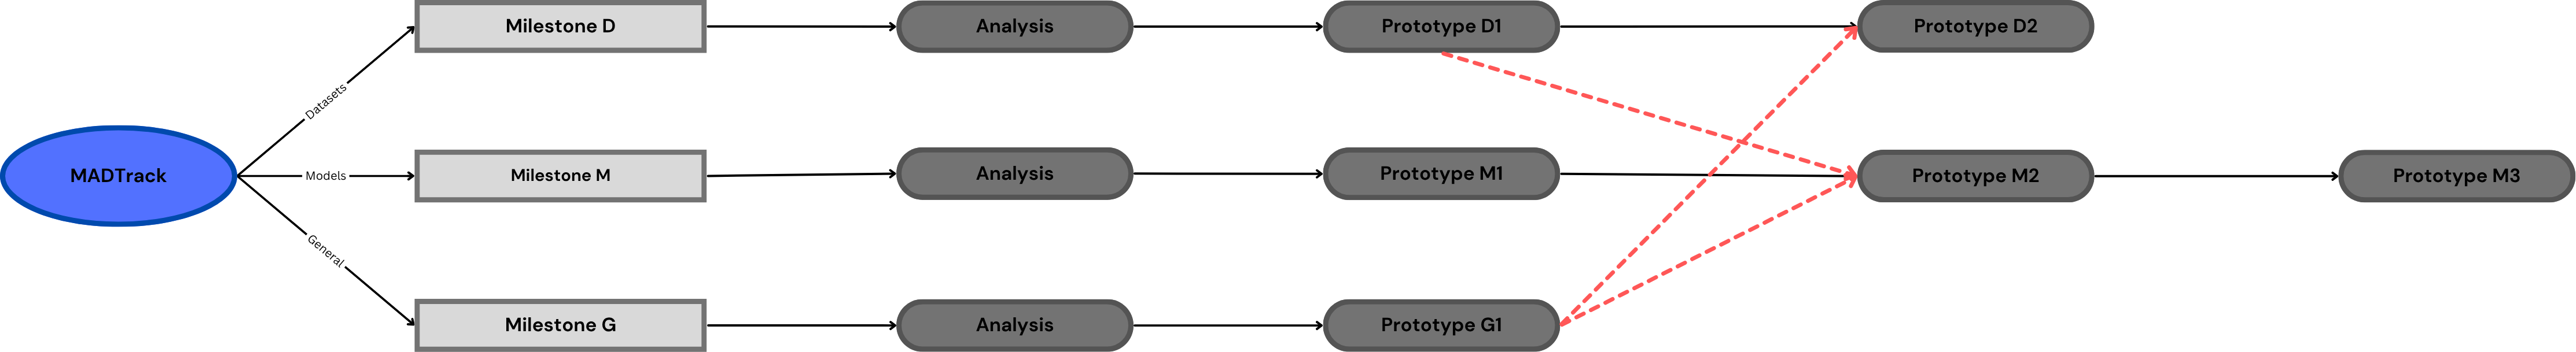
\includegraphics[width=\linewidth]{figs/MADTrack-roadmap.png}
    \caption{Iteration roadmap of the MADTrack project.}
    \label{fig:roadmap}
\end{sidewaysfigure}

\begin{sidewaysfigure}
    \centering
    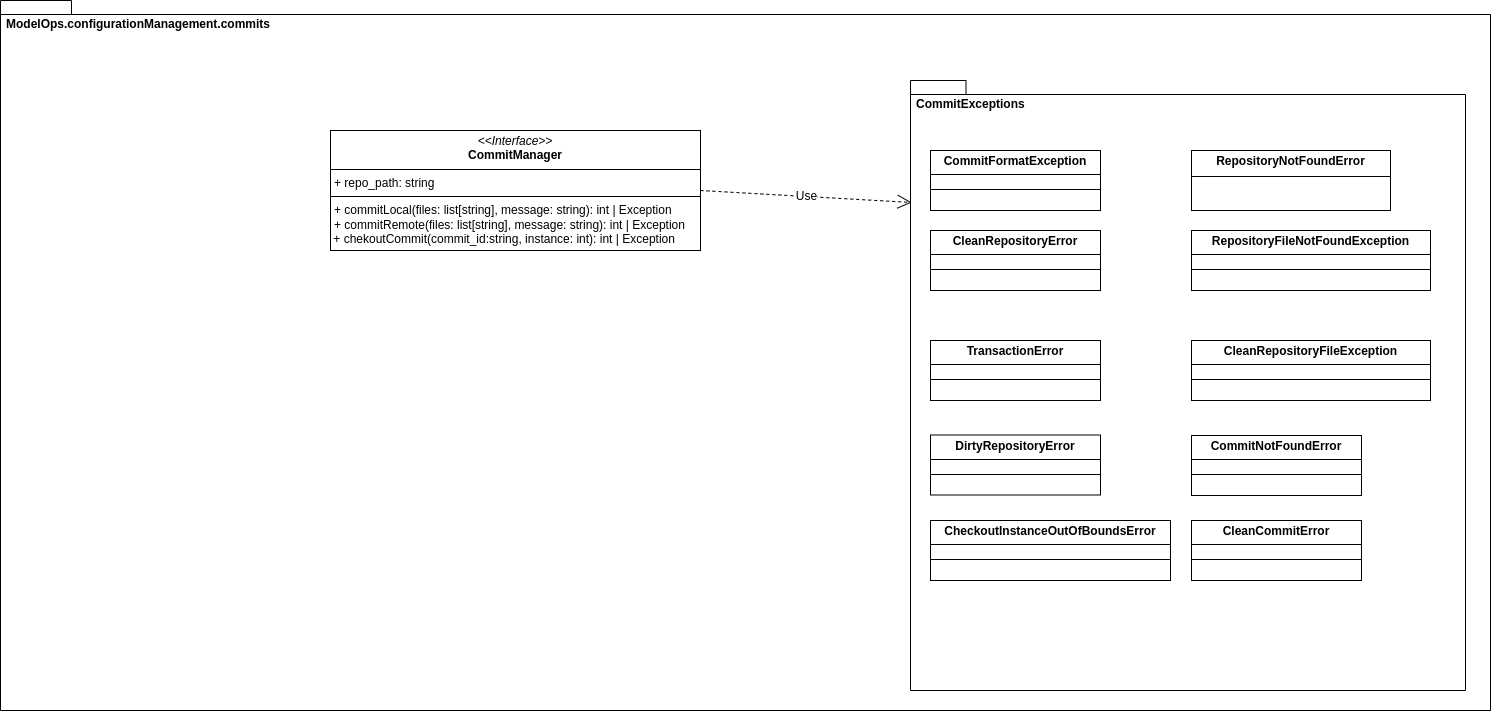
\includegraphics[width=\linewidth]{figs/G1-classDiagram.png}
    \caption{Class diagram for prototype \emph{G1}.}
    \label{fig:G1classDiagram}
\end{sidewaysfigure}
 % Apéndice A (opcionales)
\include{./Anexos/AnexoB} % Apéndice A (opcionales)
%--- (FIN DOCUMENTO)
\end{document}